% Summary of the report
% Victor Manuel Fernandez Castro
% 4 April 2016

\documentclass[10pt,a4paper]{article}

\usepackage[utf8]{inputenc}
\usepackage[spanish]{babel}
\usepackage{graphicx}
\usepackage{fancyhdr}
\usepackage{multicol}
\usepackage[skip=6pt]{caption}
\usepackage[hidelinks]{hyperref}
\usepackage{multirow}
\usepackage[T1]{fontenc}
\usepackage{enumitem}

\title{Interpretación remota de partituras sobre instrumentos de viento}
\author{Víctor Manuel Fernández Castro}
\date{Abril de 2016}

\setlength{\parskip}{6pt}
\fancyhead[L]{Víctor M. Fernández Castro}
\renewcommand{\footrulewidth}{0.4pt}
\setlength{\headheight}{13.07225pt}

% ------------------------------------------------------------------------------

\begin{document}
	
	% Portada ------------------------------------------------------------------
	
	\thispagestyle{empty}
	
	\begin{center}
		
\includegraphics[scale=0.2]{images/logo_ugr}
	\par\end{center}
	
	\begin{center}
		ESTUDIOS DE INGENIERÍA EN INFORMÁTICA
	\end{center}
	
	\begin{center}
		\vspace*{1cm}
	\end{center}
	
	\begin{center}
		\textbf{\emph{\Large {}``Interpretación remota de partituras sobre instrumentos de viento''}}
	\end{center}
	
	\begin{center}
		\vspace*{0.5cm}
	\end{center}
	
	\begin{center}
		REALIZADO POR:
	\end{center}
	
	\begin{center}
		\textbf{Víctor Manuel Fernández Castro}
	\end{center}
	
	\begin{center}
		\vspace*{0.5cm}
	\end{center}
	
	\begin{center}
		DIRIGIDO POR:
	\end{center}
	
	\begin{center}
		\textbf{Andrés María Roldán Aranda} \\
		Y \\
		\textbf{María Isabel García Arenas}
	\end{center}
	
	\begin{center}
		\vspace*{0.5cm}
	\end{center}
	
	\begin{center}
		DEPARTAMENTOS:
	\end{center}
	
	\begin{center}
		\textbf{Electrónica y Tecnología de Computadores} \\
		\textbf{Arquitectura y Tecnología de Computadores}
	\end{center}
	
	% Índice -------------------------------------------------------------------
	
	\newpage
	\tableofcontents
	
	% Capítulo 1 ---------------------------------------------------------------
	
	\newpage
	\pagestyle{fancy}
	\section{Introducción y objetivos}
	
	Nuestro proyecto parte de la atención en numerosas iglesias de Granada, que
	incorporan órganos de tubos, instrumentos muy complejos, muchos de ellos
	formando parte del inmobiliario, y merecedores de un gran reconocimiento por
	la artesanía y la calidad de su construcción.
	
	Lamentablemente, muchos de ellos se encuentran en un estado de abandono, lo
	que acelera su deterioro, no se reparan y, por ello, no se pueden tocar,
	cayendo en un círculo vicioso.
	
	Además, creemos interesante la idea de que se pueda hacer sonar un órgano
	aunque no haya organista, dando la posibilidad tanto de acompañar
	celebraciones litúrgicas como de tener música de fondo durante el horario de
	visitas.
	
	\subsection{Objetivos}
	
	Nuestro propósito es ingeniar un sistema capaz de \textbf{interpretar
	partituras musicales en un órgano} suplantando las pulsaciones del artista,
	lo que incluye los siguientes objetivos:
	
	\begin{enumerate}
		\item Analizar la \textbf{mecánica real} de un órgano eclesiástico.
		
		\begin{enumerate}
			\item Tomar \textbf{medidas completas} de cada uno de los teclados,
			los pedales y las palancas de registros.
			\item \textbf{Diseñar en 3D} los componentes principales del
			instrumento.
			\item Determinar la \textbf{presión} necesaria para mover cada
			tecla, cada pedal y cada palanca del órgano.
		\end{enumerate}
		
		\item Estudiar la comunicación entre el \textit{software} y el
		\textit{hardware}, incluyendo todos los \textbf{componentes
		electrónicos} que habrá de incluir.
		
		\item Plantear distintas \textbf{alternativas de sistemas empotrados}
		que sirvan de soporte de programación.
		
		\item Analizar el \textbf{protocolo MIDI} como formato de archivo para
		almacenar partituras.
		
		\item \textbf{Diseñar} el sistema \textit{software} que cubrirá varias
		vías de comunicación entre el usuario y la mecánica, lo que comprende:
		
		\begin{enumerate}
			\item Un \textbf{servicio en segundo plano}, que atienda:
			
			\begin{enumerate}
				\item Reproducción de archivos MIDI.
				\item Comunicación inter-proceso.
				\item Receptor de un mando a distancia.
				\item Menú de control sobre el hardware, con un ''modo
				Ingeniería''.
			\end{enumerate}
			
			\item Una \textbf{aplicación \textit{web}} para controlar el
			sistema, con soporte para:
			
			\begin{enumerate}
				\item Reproducir partituras electrónicas.
				\item Instalar nuevas piezas y gestionar listas de reproducción.
				\item Configurar el mando a distancia.
			\end{enumerate}
			
			\item Una \textbf{base de datos} como soporte de almacenamiento
			persistente.
			\item Un \textbf{protocolo de comunicación} entre la aplicación
			y el servicio.
		\end{enumerate}
		
		\item \textbf{Implementar} el sistema diseñado, como:
		
		\begin{enumerate}
			\item Un demonio para Linux.
			\item Un servicio \textit{web} sobre Apache y PHP.
			\item Una base de datos MySQL.
		\end{enumerate}
		
		\item \textbf{Validar} junto al \textit{hardware} el proyecto
		desarrollado.
	\end{enumerate}
	
	El diseño del sistema electrónico, que requiere competencias de Ingeniería
	Electrónica e Industrial, fue objeto del proyecto de D. Mikel Aguayo
	Fernández.
	
	% Capítulo 2 ---------------------------------------------------------------
	
	\section{Requisitos técnicos}
	
	Para especificar el diseño de este proyecto hemos propuesto una serie de
	requisitos tanto \textit{hardware} como \textit{software}, que enumeramos a
	continuación.
	
	\subsection{Requisitos hardware}
	
	\begin{enumerate}
	
		\item Un juego de mecanismos accionará las \textbf{teclas}, otro moverá
		los \textbf{pedales} y otro desplazará los \textbf{registros} de
		timbres.
		
		\item El sistema no podrá acceder a la mecánica interna del instrumento,
		ni modificarlo de ninguna forma.
		
		\item No podrá apoyarse demasiado peso sobre el órgano, ni hacerse
		contra-apoyo (hacia arriba).
		
		\item El \textbf{control principal}, la instalación de partituras y la
		configuración se harán \textbf{remotamente}.
		
		\item Se proveerá un \textbf{control local reducido} de los accionadores
		con fines de puesta en marcha y mantenimiento.
		
		\item Asimismo se facilitará el control remoto desde un \textbf{mando a
		distancia}.
		
		\item El diseño debe ser \textbf{flexible y extensible} para distintos
		órganos.
		
		\item Se debe de poder instalar y desinstalar fácilmente.
		
	\end{enumerate}
	
	\subsection{Requisitos software}
	
	\begin{enumerate}
		
		\item Se ofrecerá \textbf{control remoto} para todos los casos de uso a
		nivel de usuario.
		
		\item La interfaz permitirá controlar la \textbf{reproducción}: iniciar
		una pieza, pausarla, reanudarla y detenerla. La reproducción por defecto
		será en modo bucle.
		
		\item Facilitará la subida y \textbf{gestión de partituras}. En dicho
		gestor se mostrará la duración de cada pieza.
		
		\item Los archivos a procesar son de formato \textbf{MIDI estándar}, sin
		perjuicio de que una partitura pueda estar adaptada específicamente al
		sistema.
		
		\item Las piezas musicales se clasificarán en \textbf{listas de
		reproducción}.
		
		\item La interfaz de usuario permitirá \textbf{asignar} dichas listas a
		ciertos botones del mando arriba mencionado.
		
		\item El \textbf{mando} tendrá capacidad para reproducir una serie de
		listas programadas, así como pausar y detener la reproducción.
		
		\item El \textit{software} dará soporte al \textbf{testeo} de los
		accionadores de forma local.
		
		\item El controlador debe ser \textbf{extensible} para órganos con más o
		menos teclas, distinto número de teclados o diferente configuración de
		registros.
		
		\item La aplicación para el usuario debe ser lo más \textbf{sencilla e
		intuitiva} posible.
		
		\item Se busca obtener una aplicación de control
		\textbf{multiplataforma}.
		
		\item La interfaz de usuario se presentará en varios \textbf{idiomas}.
		
		\item Ya que el control es remoto, se hará hincapié en la
		\textbf{seguridad}, tanto autentificación de acceso como aspectos de
		programación, tales como inyección de código.
		
	\end{enumerate}
	
	% Capítulo 3 ---------------------------------------------------------------
	
	\section{Análisis del sistema}

	Como paso previo al diseño del sistema, deberemos conocer con detalle todos
	los elementos con los que va a interactuar nuestro sistema, así como
	plantear diferentes alternativas de cara al desarrollo del
	\textit{software}.

	\subsection{Órgano de la Parroquia de Santa Fe}

	El instrumento instalado en la Parroquia de la Encarnación de Santa Fe es en
	realidad un doble órgano artesanal construido en dos fases: En 1775 se
	instaló el primer órgano, de estilo \textbf{barroco}, obra del organero
	Pedro Ghys. Posteriormente, a principios de la década de 1830, el francés
	Guillermo D'Enoyer lo amplía añadiendo un órgano \textbf{romántico}, con un
	segundo teclado y nuevos sonidos, pero todo el mecanismo es independiente
	del primer instrumento.
	
	\begin{multicols}{2}
		\noindent
		\begin{center}
			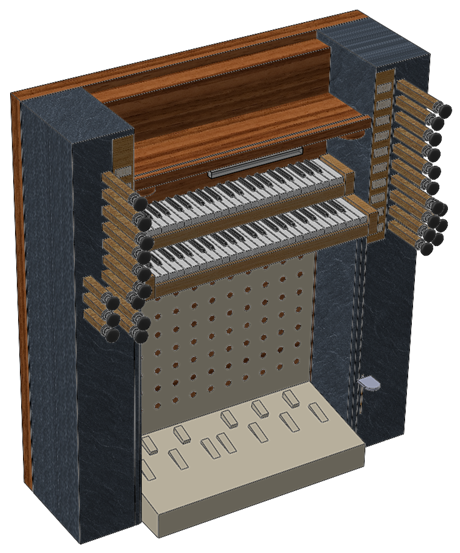
\includegraphics[width=0.45\textwidth]{images/organo} 
			\captionof{figure}{Reproducción 3D del órgano.}
		\end{center}
		\columnbreak
		Para funcionar, el órgano se alimenta de \textbf{aire}. Antiguamente se utilizaba un fuelle gigante, situado en la antesala, que llevaba el aire a una cámara de almacenamiento, para proporcionar un flujo de entrada constante. Hoy día el fuelle ha sido sustituido por una \textbf{bomba eléctrica}.
		
		La primera tarea que llevamos a cabo fue conocer el órgano en profundidad, tomar algunas medidas y \textbf{diseñar el modelo en 3D} con el \textit{software} \textit{SolidWorks}.
	\end{multicols}
	
	\begin{multicols}{2}
		\noindent
		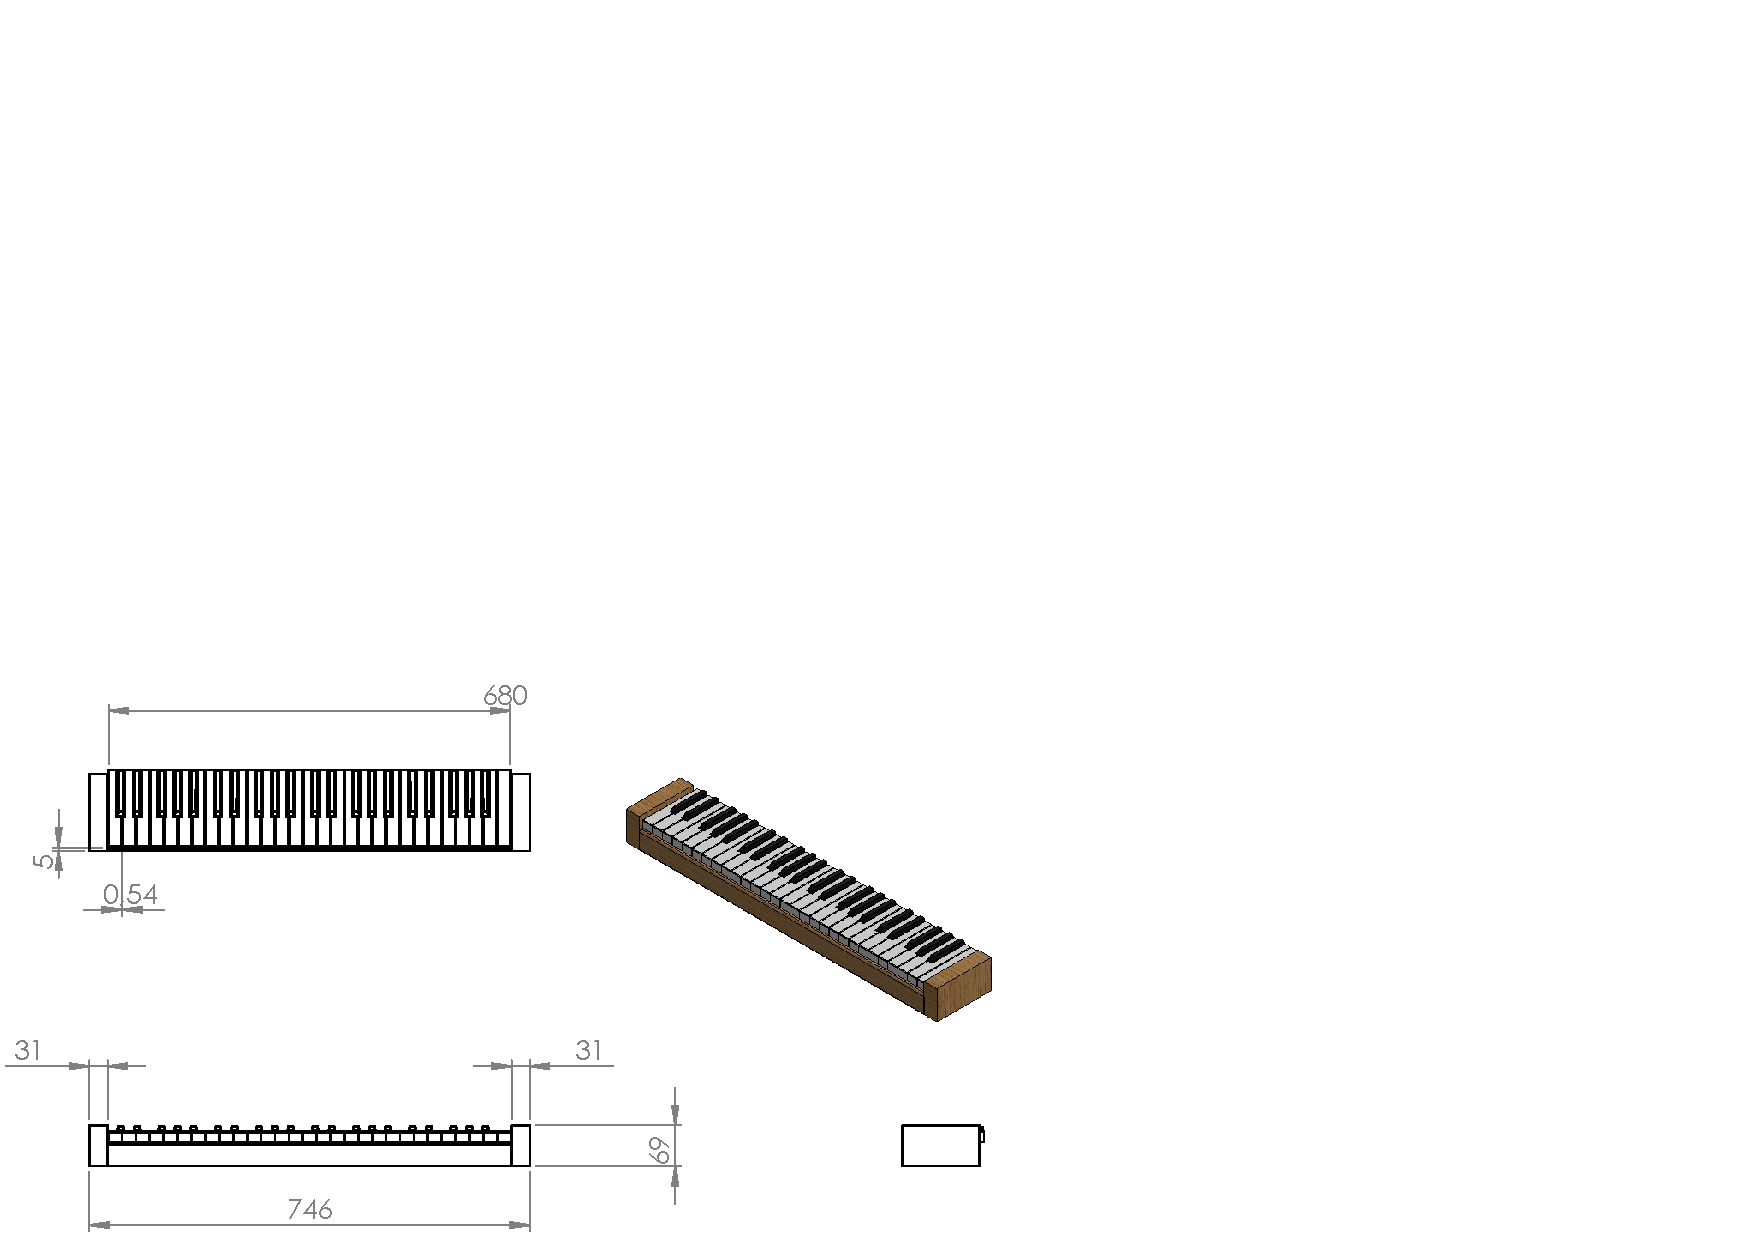
\includegraphics[width=0.45\textwidth]{images/teclado_modelo} 
		\captionof{figure}{Medidas del teclado.}
		\columnbreak
		Tenemos dos teclados de cuatro octavas notas cada uno, el de arriba, correspondiente al órgano barroco, y otro más abajo, que sobresale del primero, para el órgano romántico, de la misma extensión.
	\end{multicols}
	
	\begin{multicols}{2}
		\noindent
		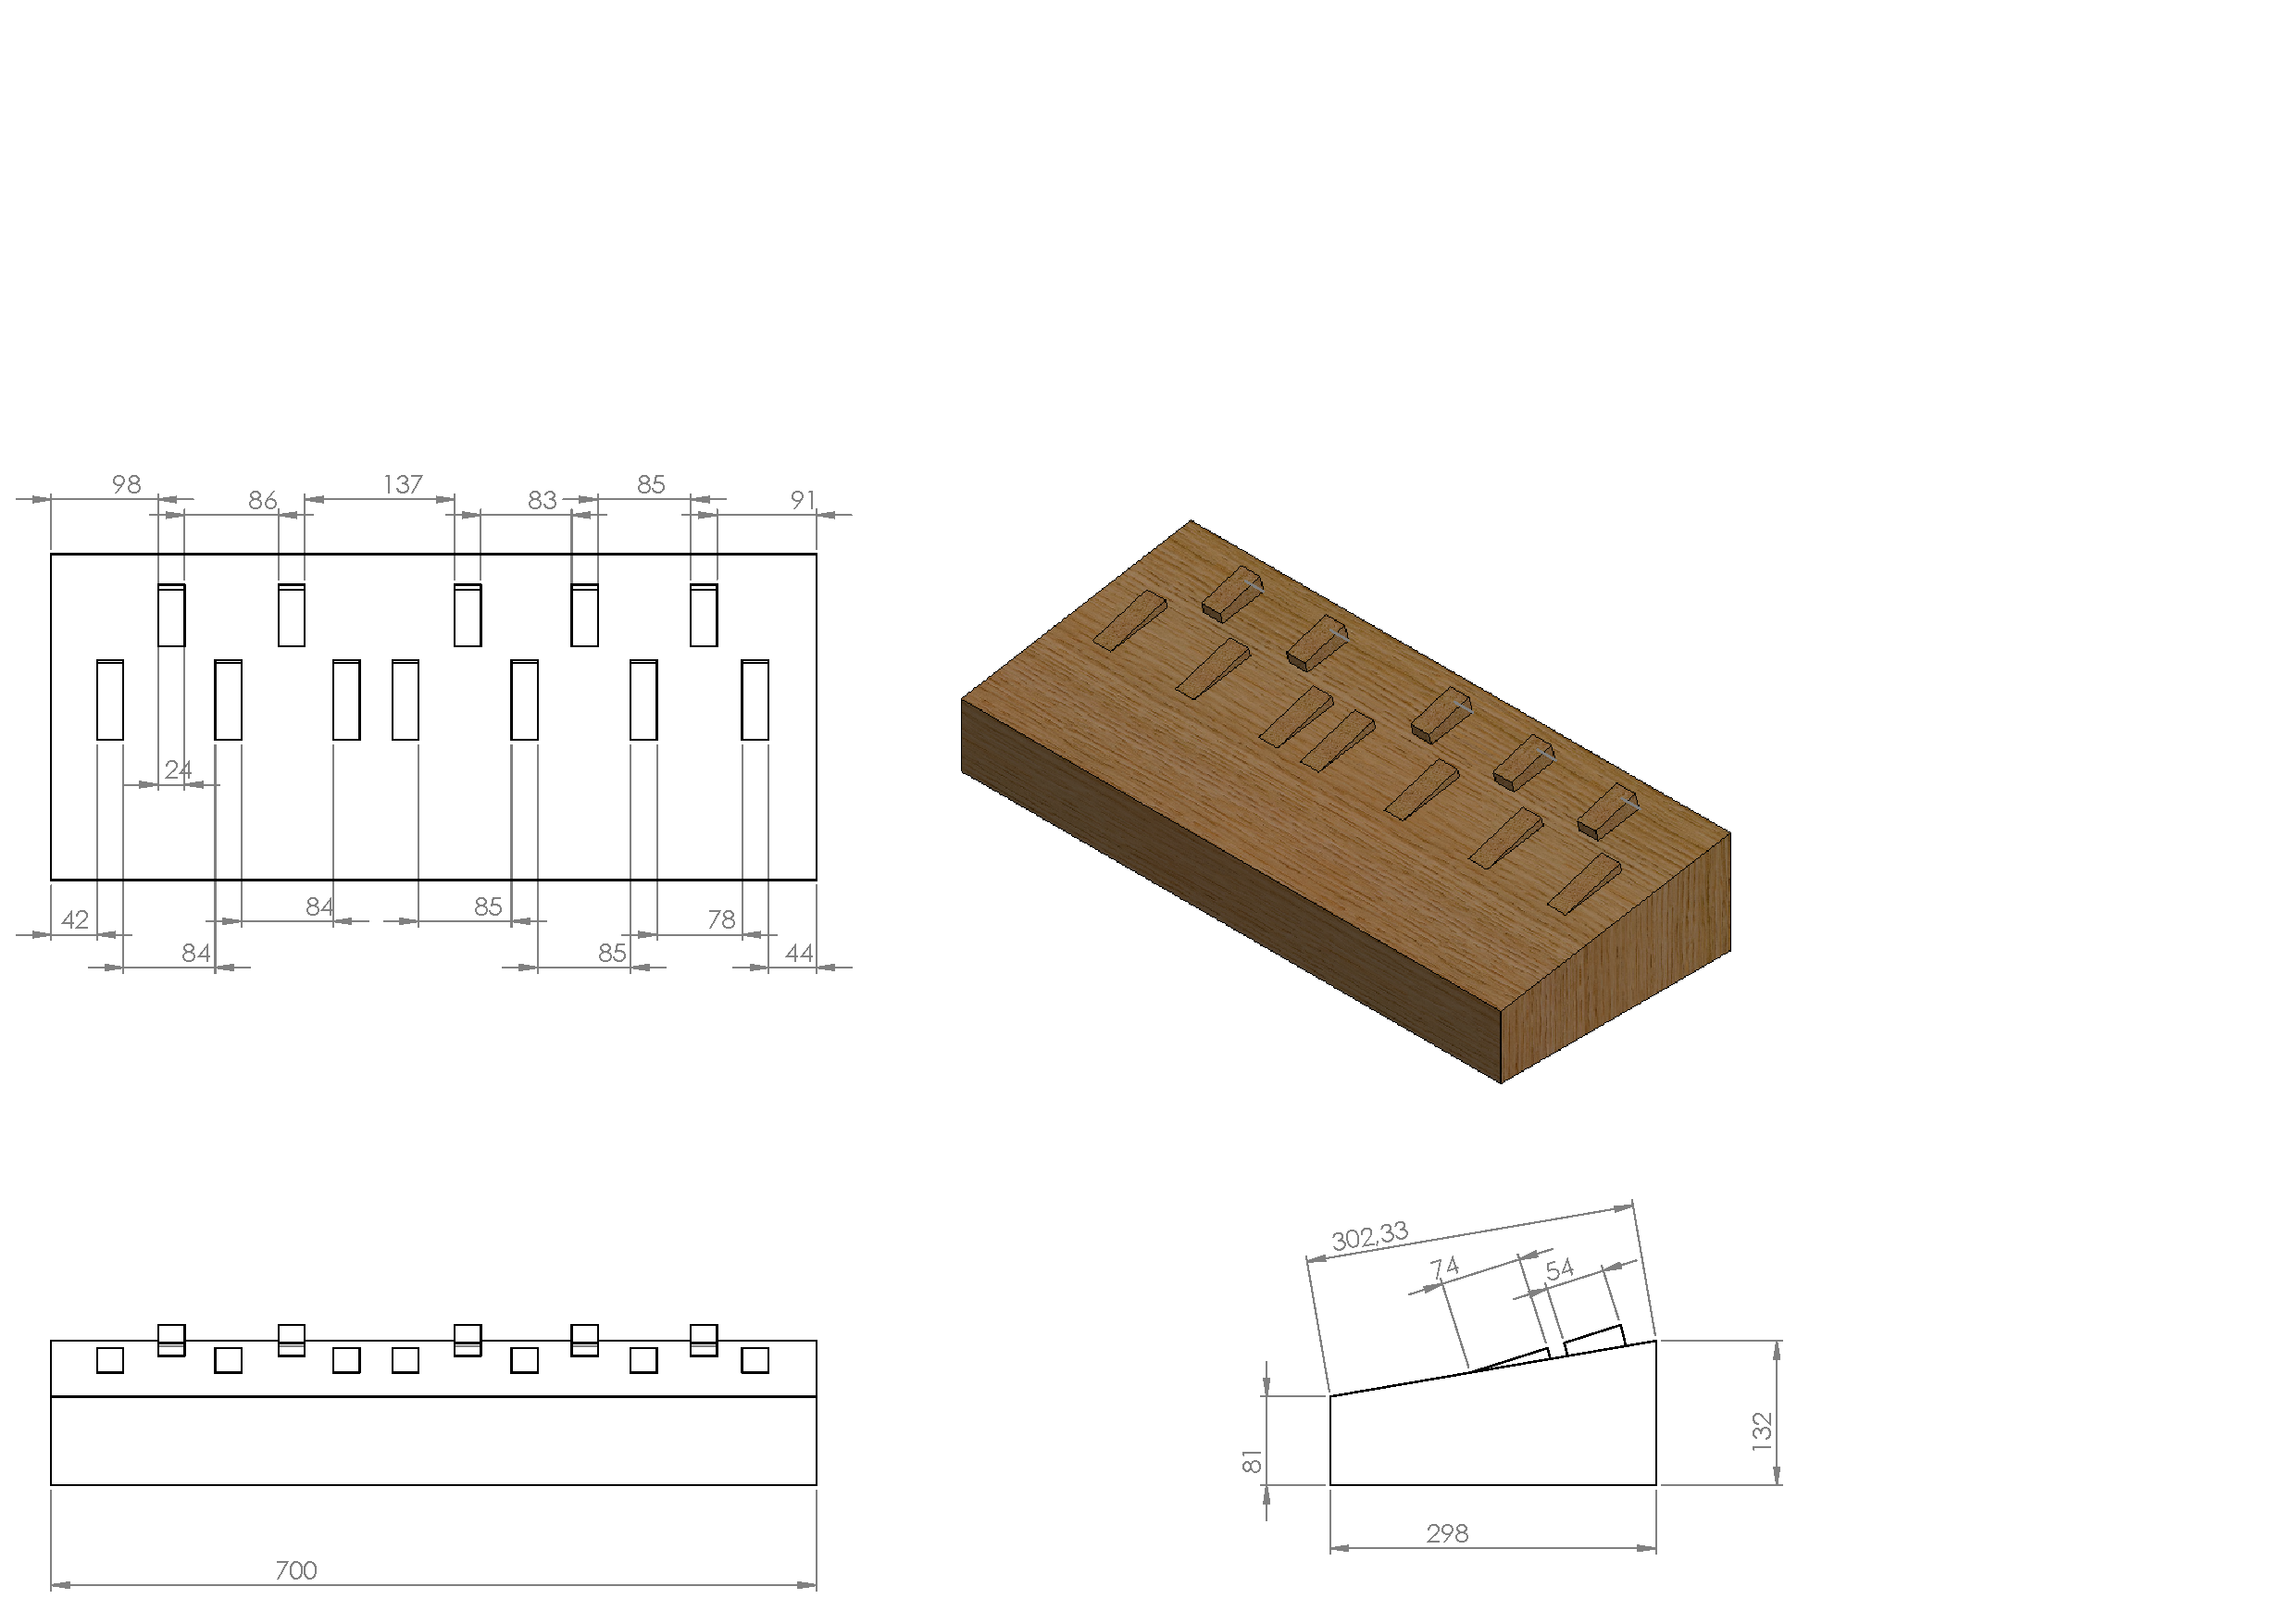
\includegraphics[width=0.45\textwidth]{images/pedalier_modelo} 
		\captionof{figure}{Medidas del pedalier.}
		\columnbreak
		Este órgano cuenta con un \textit{pedalier} con un registro fijo: el \textbf{bajo de \textit{contrast}}. Los pedales están dispuestos en forma de escala diatónica, igual que las teclas. Cada pedal tiene aproximadamente la misma anchura que una tecla aunque, obviamente, están más separados unos de otros.
	\end{multicols}
	
	\begin{multicols}{2}
		\noindent
		\begin{center}
			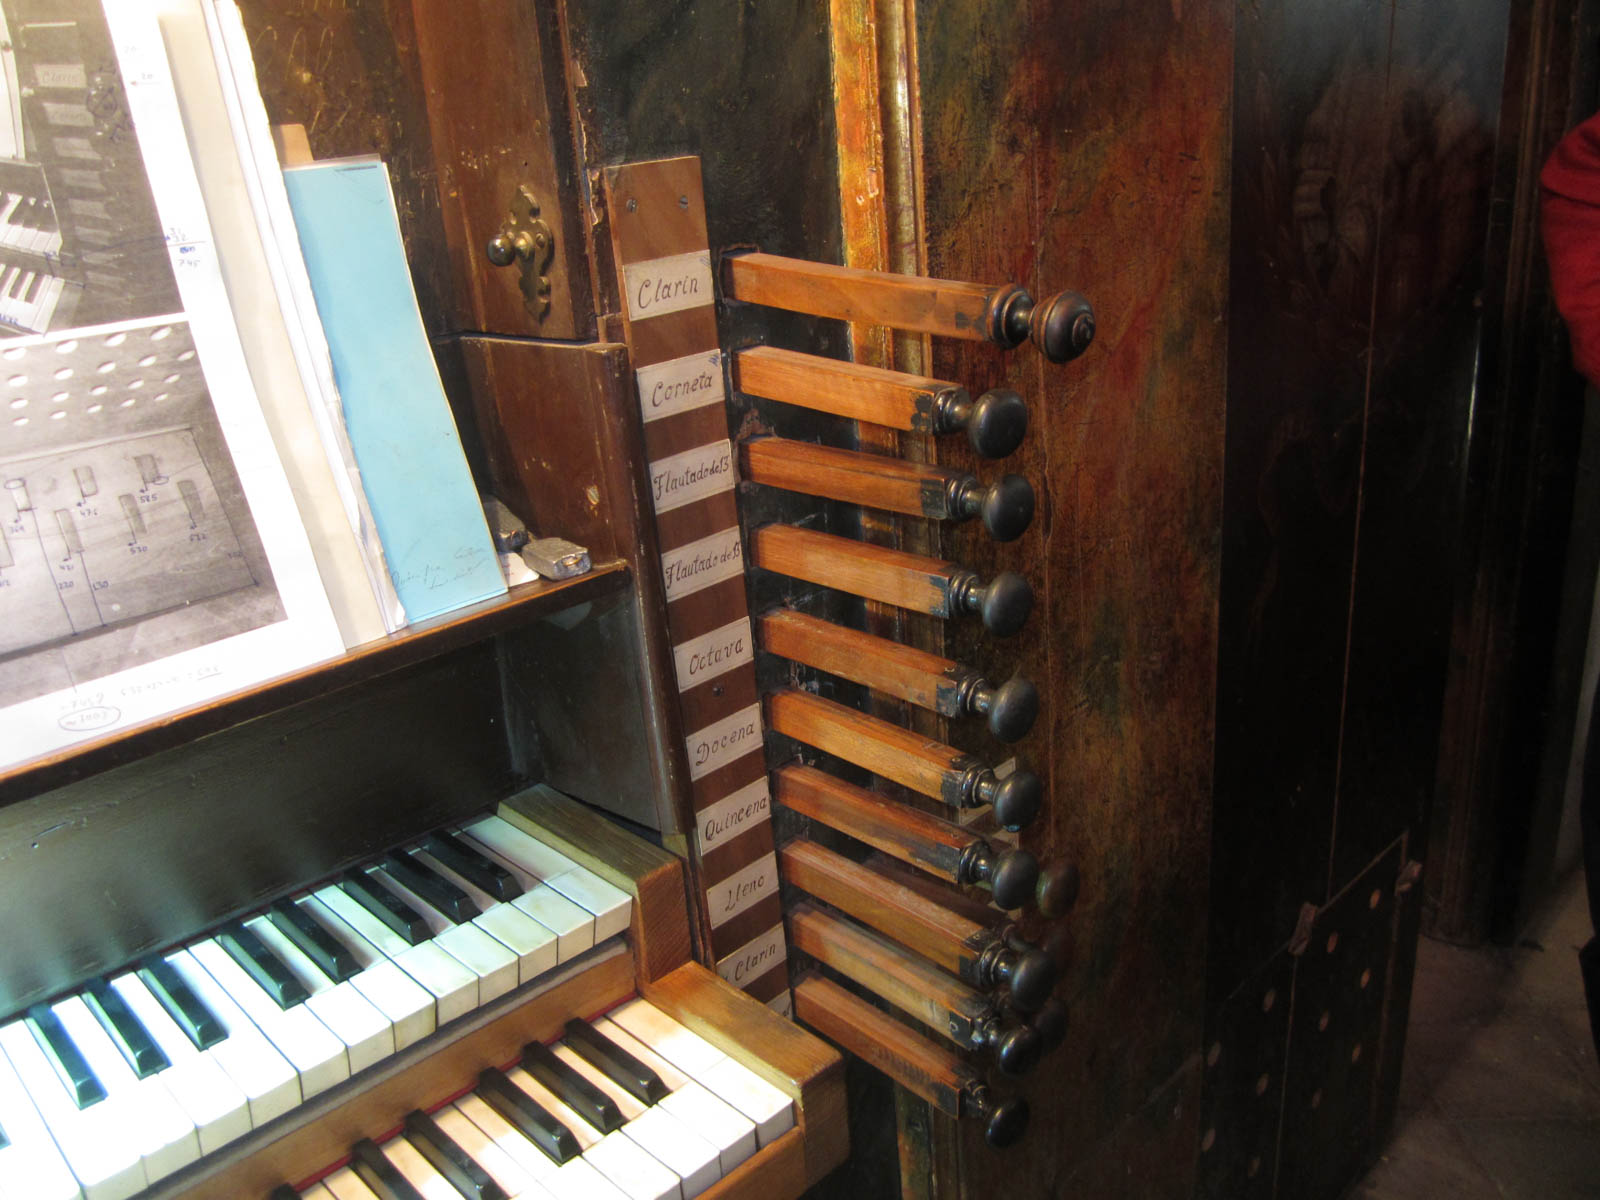
\includegraphics[width=0.45\textwidth]{images/registros} 
			\captionof{figure}{Hilera de registros barrocos.}
		\end{center}
		\columnbreak
		Los registros son las diferentes \textbf{familias de tubos} con el mismo timbre y la misma tesitura. Se pueden abrir o cerrar desde la consola a través de una serie de palancas, de las que se tira para hacer sonar el registro o se empuja para silenciarlo.
	\end{multicols}
	
	\subsection{PCB de control}
	
	\begin{multicols}{2}
		La placa de circuito impreso es la solución a los requisitos \textit{hardware} aportada por el \textbf{proyecto de Mikel Aguayo Fernández}. 
		
		Incluye una serie de registros de desplazamiento para almacenar el estado del órgano, una interfaz de control local reducido y un medio de control remoto. También alimentará al computador que vamos a utilizar. 
		
		A continuación enumeramos aquellos componentes con los que interactuaremos:
		\columnbreak		 
		\begin{center}
			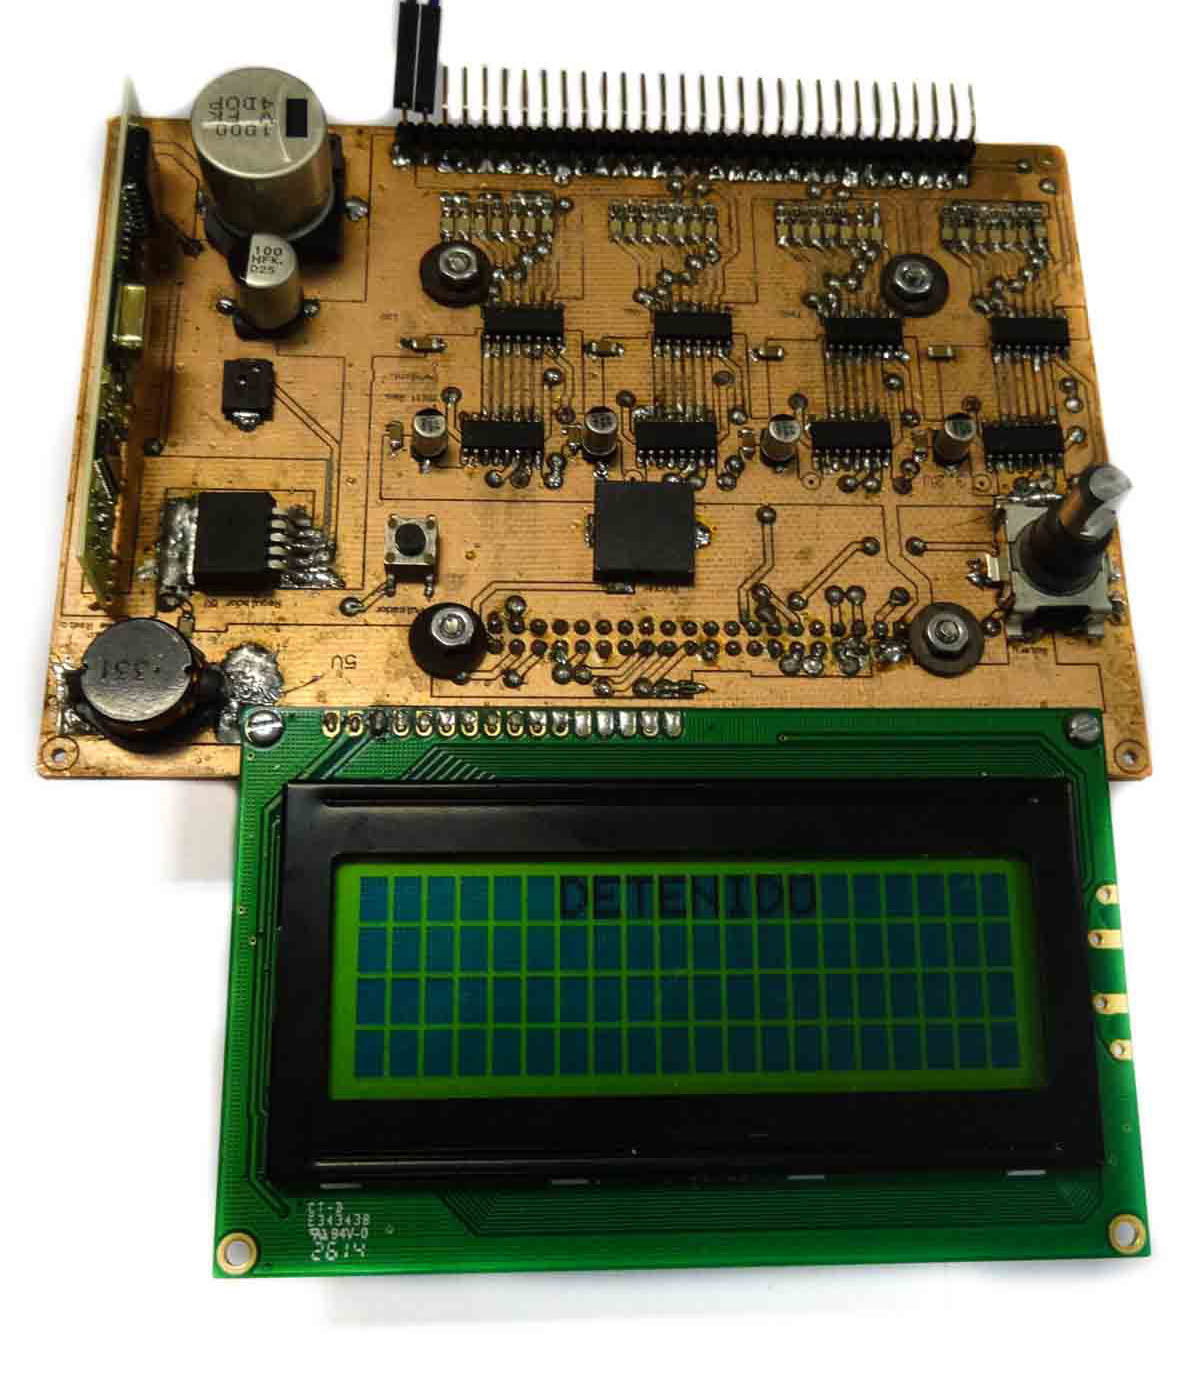
\includegraphics[width=0.45\textwidth]{images/pcb} 
			\captionof{figure}{Prototipo hardware.}
		\end{center}
	\end{multicols}	
	
	\begin{description}
		\item[Registros de desplazamiento SN74HC595.] Son circuitos lógicos que almacenan una serie de bits. Este modelo, con una capacidad de 8 bits, soporta entrada en serie y salida en paralelo. Usaremos \textbf{cuatro registros} de desplazamiento: uno para cada teclado, otro para el \textit{pedalier} y otro para los registros.
		
		\item[Receptor RF HIRK-433A.] Es un detector de radio con decodificador a interfaz RS-232. Nos da la información del \textbf{número de serie} del mando y qué \textbf{botones} han disparado el evento. 
		
		\item[Pantalla LCD FDCC2004B.] Es un dispositivo genérico de 4 x 20 caracteres. Tiene una pequeña \textbf{memoria} para almacenar el estado e incluye los caracteres ASCII predefinidos.
		
		\item[Codificador rotatorio EC11J.] Es un componente electrónico consistente en un \textbf{botón giratorio y pulsable}. Emite una señal que depende del sentido en que se ha girado el botón.
		
		\item[Zumbador PKLCS1212E4001-R1.] Es un dispositivo piezoeléctrico que produce un sonido agudo continuado. A diferencia de un altavoz, está diseñado para producir \textbf{ondas cuadradas}.
	\end{description}
	
	\subsection{SBC Raspberry Pi}
	
	El \textit{Raspberry Pi} es un \textbf{ordenador} de placa única ---SBC---, más potente que un microcontrolador y con \textbf{sistema operativo} basado en Linux. Se alimenta por USB y se puede controlar con teclado y ratón, o bien desde red mediante SSH.
	
	\begin{multicols}{2}
		\noindent
		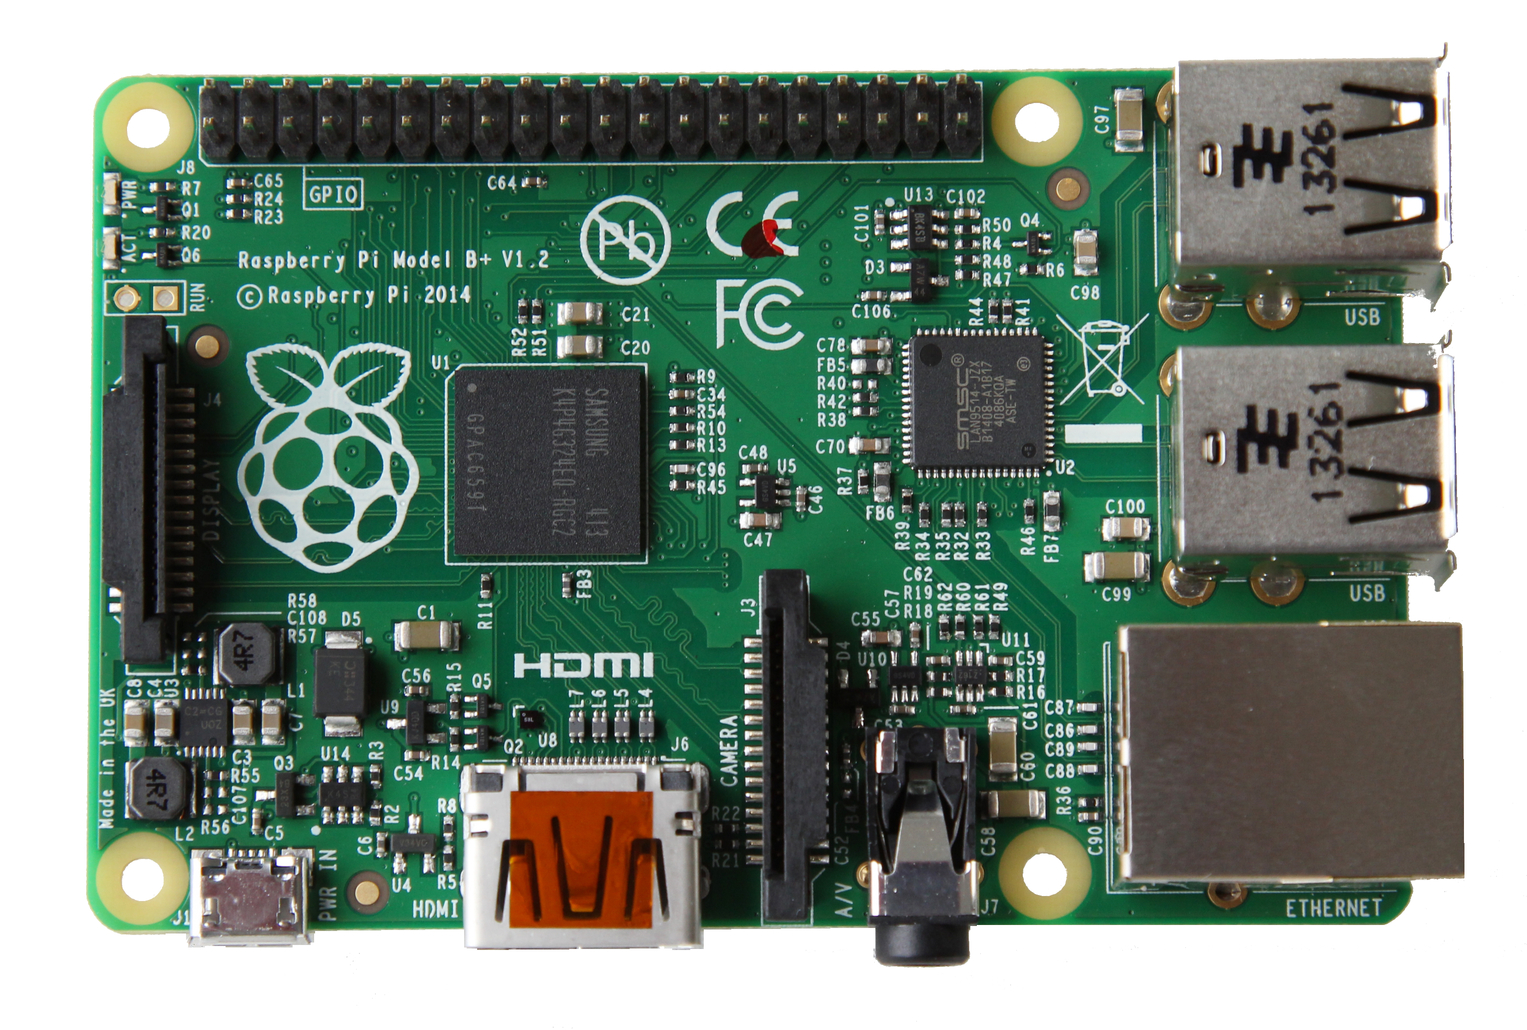
\includegraphics[width=0.45\textwidth]{images/raspberry} 
		\captionof{figure}{Raspberry Pi modelo B.}
		\columnbreak
		El corazón de este computador es un SOC, que integra microprocesador, memoria y periféricos principales.
		
		El modelo escogido, \textit{B+}, posee numerosos pines de entrada y salida de propósito general (GPIO), que utilizaremos para interactuar con la PCB y para ser \textbf{alimentado} por ésta.
	\end{multicols}
	
	 La PCB se conectará al \textit{Raspberry Pi} a través de los conectores GPIO. Todos ellos se utilizarán de forma \textbf{genérica}, excepto el receptor del mando a distancia, que se comunica con la interfaz RS-232 y debe conectarse al \textbf{UART} mediante el pin dedicado a tal periférico.
	 
	 \begin{center}
	 	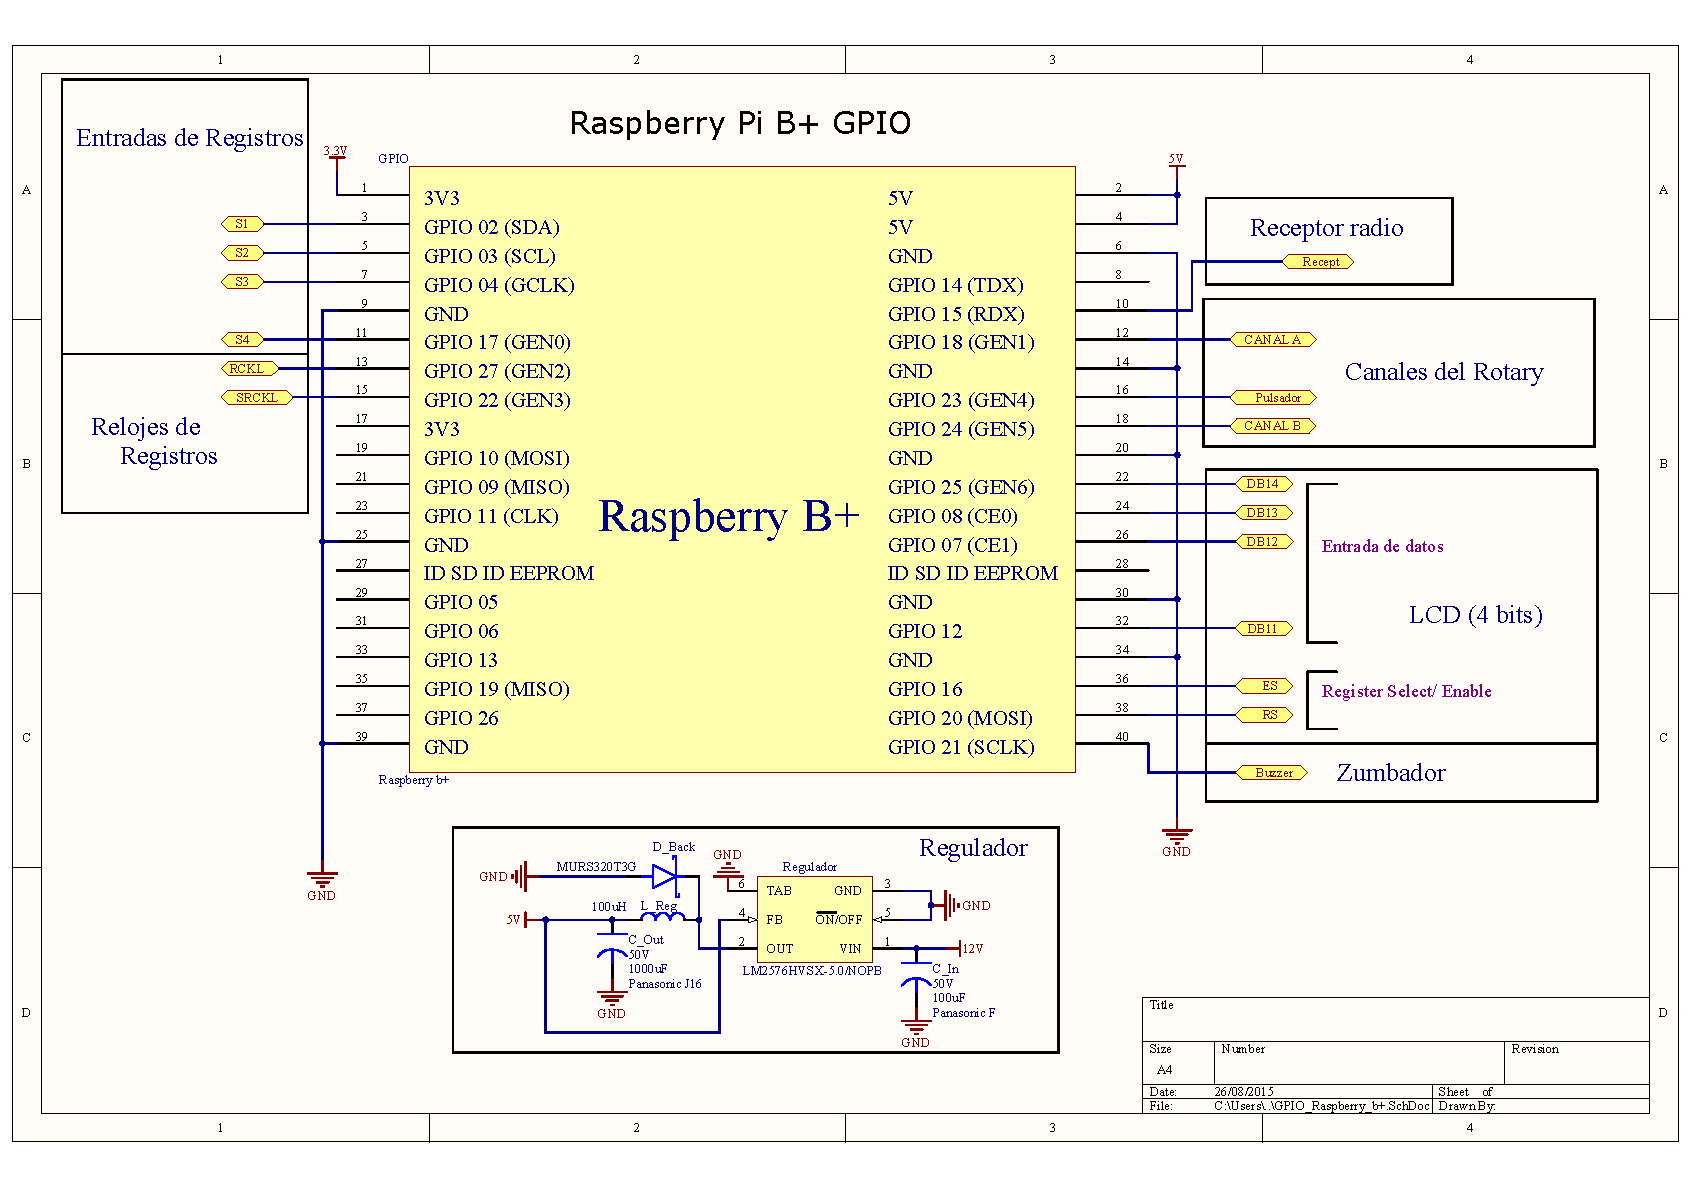
\includegraphics[width=0.75\textwidth]{images/pcb_gpio}
	 	\captionof{figure}{Pines de conexión de la PCB con el Raspberry Pi.}
	 \end{center}
	
	\subsection{Formato de archivo MIDI}
	
	Los datos de entrada a nuestro sistema consisten en archivos MIDI, tal como se menciona en los requisitos. Este tipo de ficheros se presenta como un conjunto de \textbf{bloques} ---\textit{chunks}--- que contienen los eventos clasificados por pistas. Todos los valores numéricos están en formato \textbf{\textit{big-endian}}, detalle a tener en cuenta, ya que tanto la arquitectura x86 como ARM trabajan en \textit{little-endian}.
	
	\begin{description}
		\item[Bloque de cabecera.] Es siempre el \textbf{primero}, empieza por la firma ''MThd'' e incluye el formato, el número de pistas y la división de tiempo.
		
		\item[Bloque de pista.] Consta de una cabecera y de una lista de eventos, que termina con el meta-evento \textit{fin de pista}.
		
		\item[Eventos MIDI.] Cada evento indica el retraso de tiempo respecto al evento anterior, el tipo de evento, el canal y los parámetros correspondientes, tales como la nota o la velocidad de pulsación.
		
		\item[Metaeventos.] Son mensajes de control que extienden la semántica de los eventos. Los más importantes son el \textbf{indicador de \textit{tempo}} y la marca de \textbf{fin de pista}.
		
		\item[Notas.] Se indican numéricamente, en base 0, asignando valores a las notas cromáticas a partir de \textit{Do -1}. Por ejemplo, al \textit{Do central (Do 4)} le corresponde el valor 60.
	\end{description}
	
	\subsection{Interconexión general}
	
	Todos los elementos que hemos descrito conformarán la parte \textit{hardware} del sistema y establecerán una conexión cuyos extremos son el \textbf{computador} \textit{Raspberry Pi} y los \textbf{mecanismos} que interactuarán con la consola del órgano.
	
	\begin{center}
		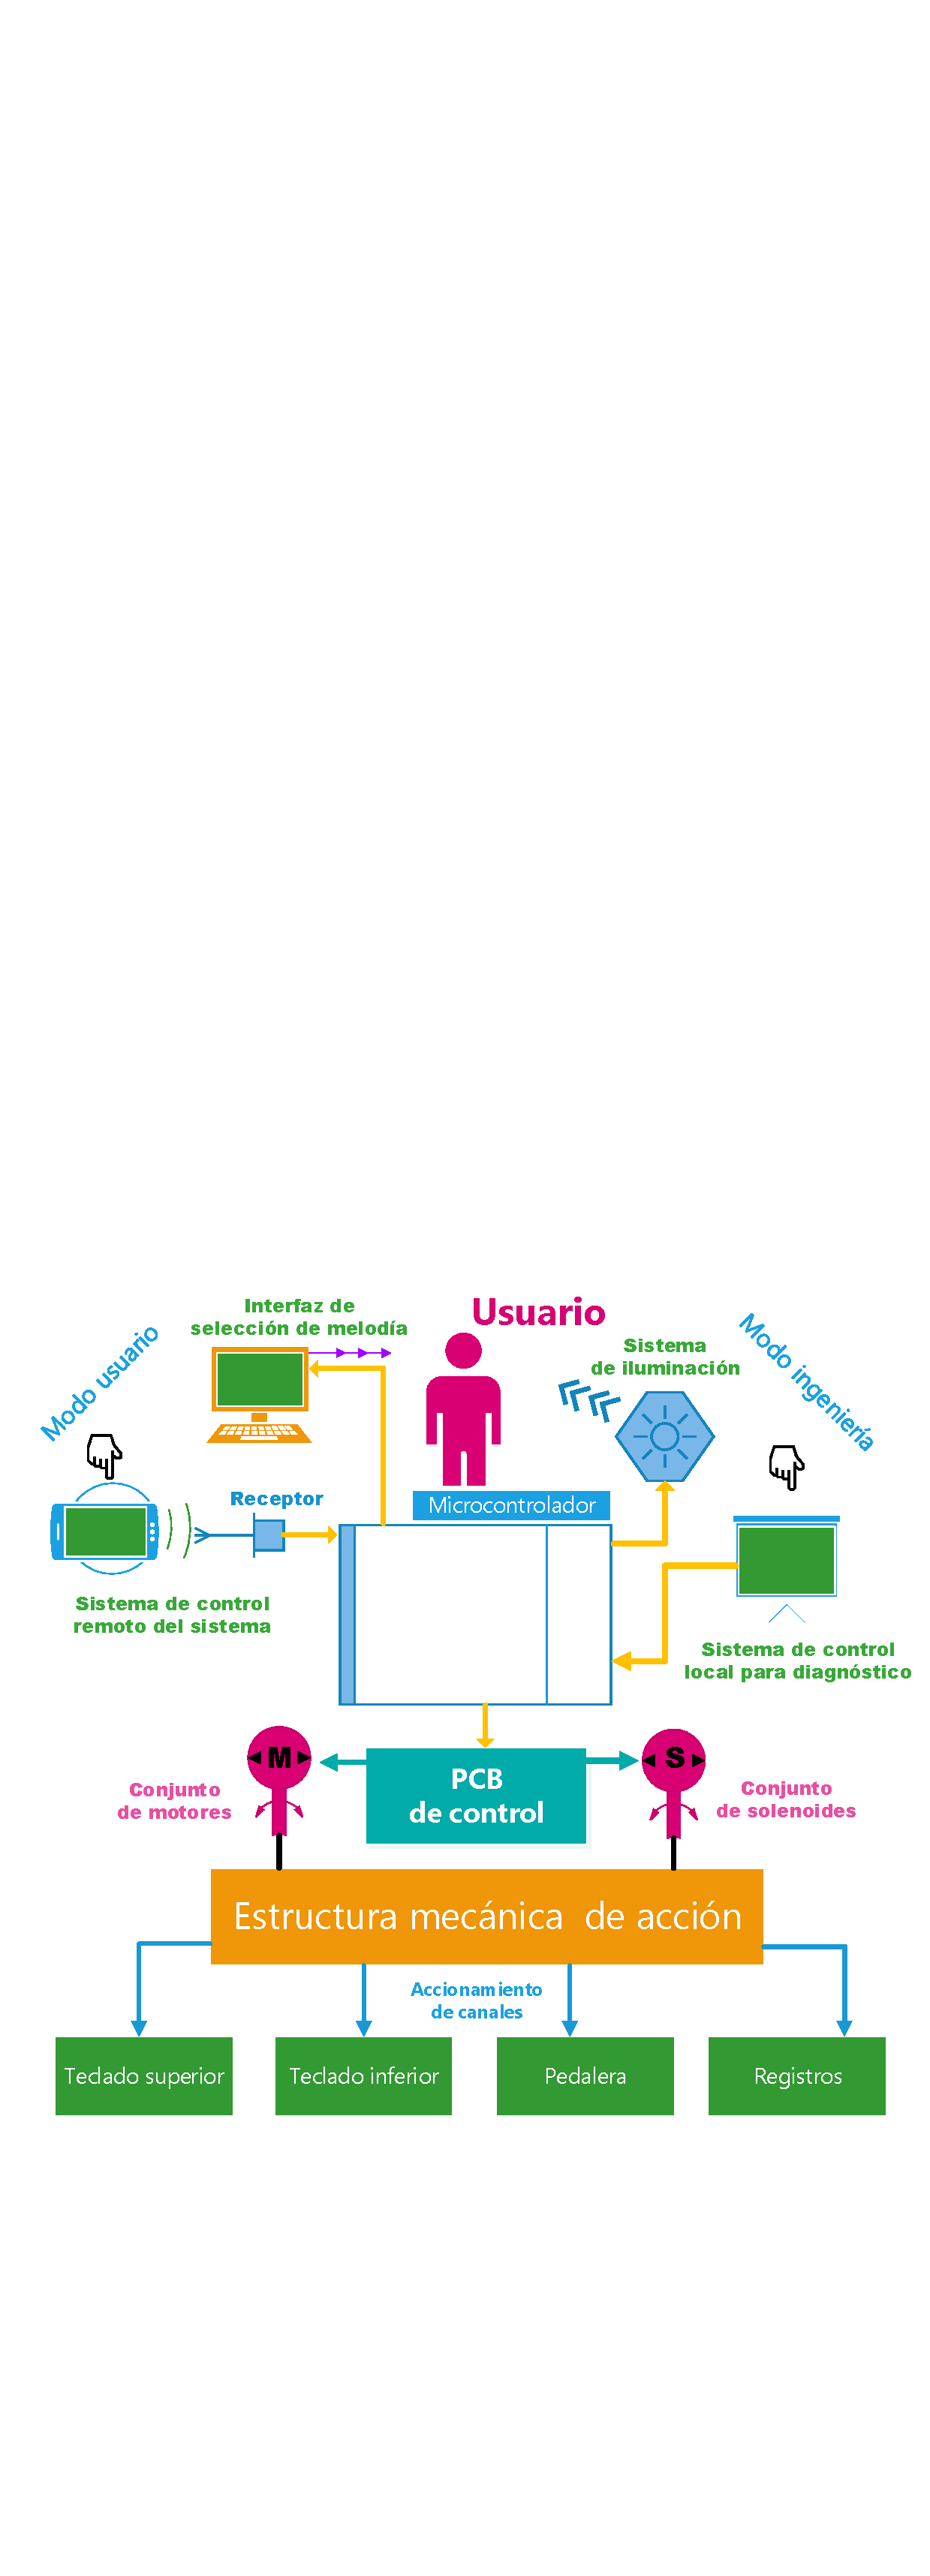
\includegraphics[width=0.75\textwidth]{images/interconexion}
		\captionof{figure}{Conexión lógica entre los elementos hardware.}
	\end{center}
	
	La PCB está conectada mediante la interfaz GPIO. Las conexiones harán funcionar los mecanismos del órgano, pasando por los registros de desplazamiento, que retendrán el estado.
	
	El resto de \textbf{periféricos} de la placa nos serán de utilidad para desarrollar un sistema que cumplirá todos los requisitos contemplados en el proyecto.
	
	% Capítulo 4 ---------------------------------------------------------------
	
	\section{Diseño e implementación}
	
	\subsection{Planteamiento}
	
	\begin{multicols}{2}
		\noindent
		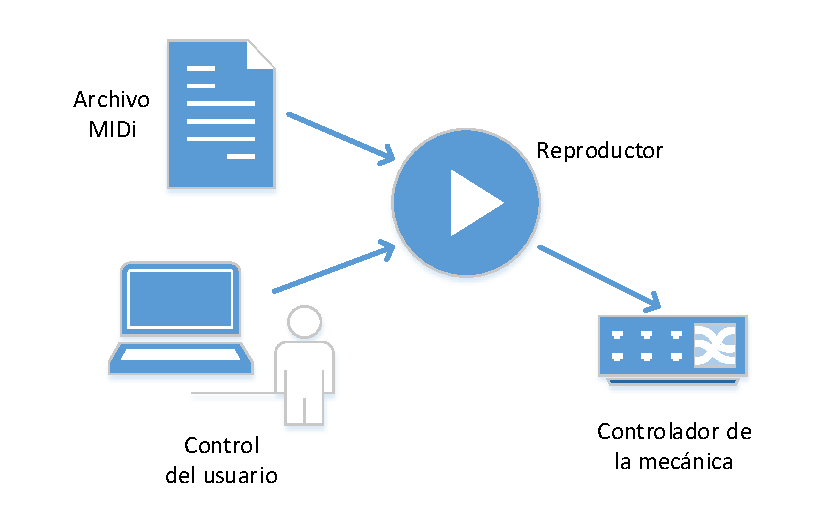
\includegraphics[width=0.45\textwidth]{images/idea} 
		\captionof{figure}{Planteamiento inicial.}
		\columnbreak
		El \textit{software} que tenemos que diseñar consiste en un \textbf{reproductor de archivos MIDI}, que recibe el fichero y lo envía a la PCB a través del GPIO.
		
		Vamos a diseñar el reproductor como un \textbf{demonio} de Linux que, además de gestionar la reproducción de archivos MIDI, proporcionará la interfaz de \textbf{control reducido}, para manejar la mecánica desde la PCB. También despachará las órdenes del \textbf{mando a distancia}.
	\end{multicols}
	
	Respecto al de \textbf{control}, se requiere varias formas de acceder al sistema:
	
	\begin{enumerate}
		\item Una \textbf{interfaz \textit{web}} como controlador principal, que cubra todos los casos de uso, y sea fácil de instalar y utilizar. Esta opción permite además que sea multiplataforma.
		
		\item Un mando a distancia, que altere la reproducción.
		
		\item Un control reducido empotrado en la PCB: el \textbf{modo ingeniero}.
	\end{enumerate}
	
	En último lugar, necesitamos \textbf{almacenar información} sobre los archivos MIDI, listas de reproducción y asignaciones del mando en memoria persistente. Una \textbf{base de datos} nos permitiría guardar toda esa información de manera estructurada y coherente, además de ser fácilmente accesible por todos los componentes del sistema.
		
	\begin{center}
		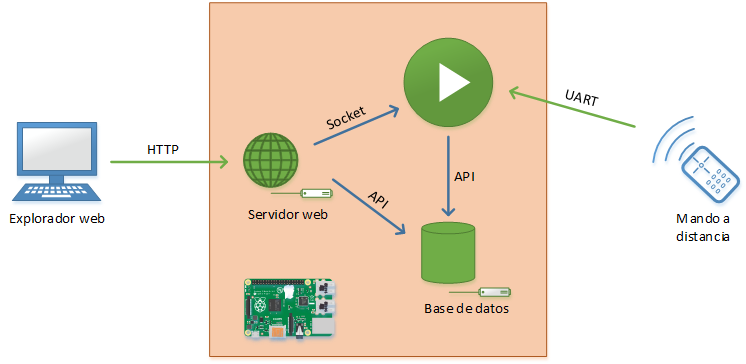
\includegraphics[width=0.75\textwidth]{images/general}
		\captionof{figure}{Diseño general.}
	\end{center}
	
	\clearpage
	\subsection{Servicio del reproductor}
	
	\begin{multicols}{2}
		\noindent
		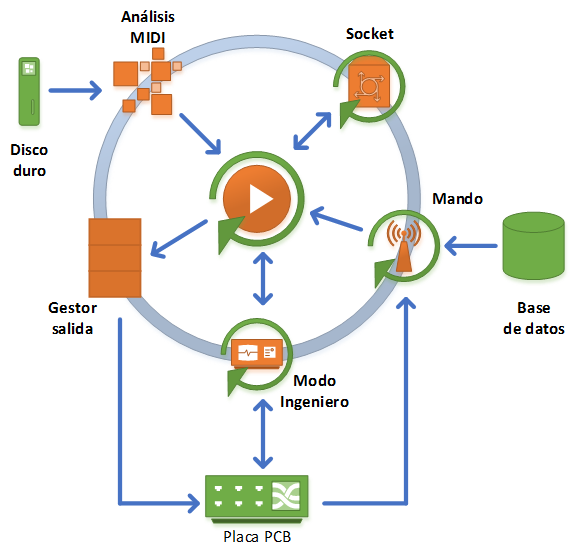
\includegraphics[width=0.45\textwidth]{images/reproductor} 
		\captionof{figure}{Diseño del reproductor.}
		\columnbreak
		El núcleo de nuestro sistema será un proceso que se ejecuta en \textbf{segundo plano}, y no interactuará directamente con el usuario, sino que se comunicará con \textbf{otros procesos} a través de los siguientes canales:
		
		\begin{enumerate}
			\item Un \textbf{\textit{socket} local} de Linux. Será usado  por la interfaz \textit{web} y por aplicaciones auxiliares.
			
			\item El \textbf{puerto en serie} (UART) del \textit{Raspberry Pi}, para recibir órdenes del mando.
			
			\item Los \textbf{pines del GPIO} correspondientes al codificador rotatorio y el LCD, para el modo ingeniero.
		\end{enumerate}
	\end{multicols}
	
	 Vamos a escribirlo casi por completo en \textbf{lenguaje C}, por su eficiencia, cercanía al \textit{hardware}, capacidad para hacer \textbf{llamadas al sistema} y la posibilidad de realizar \textbf{optimizaciones en ensamblador}.
	 
	 \begin{multicols}{2}
	 	\noindent
	 	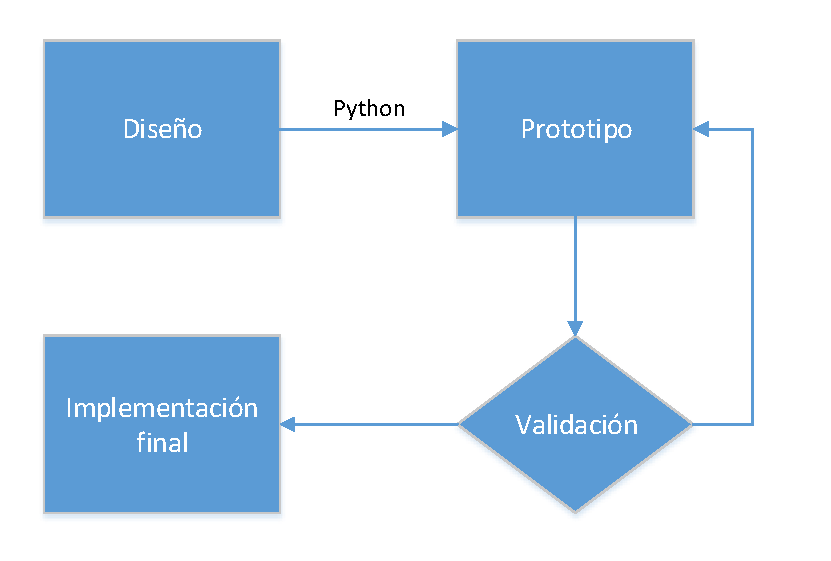
\includegraphics[width=0.45\textwidth]{images/prototipado} 
	 	\captionof{figure}{Esquema de prototipado.}
	 	\columnbreak
	 	En ciertos componentes, necesitaremos hacer \textbf{prototipos} para estudiar su funcionamiento y realizar pruebas de concepto, antes de implantarlos definitivamente. 
	 	
	 	Esto lo haremos en \textbf{Python}, un lenguaje interpretado y de programación más ágil que C.
	 \end{multicols}
	
	\subsubsection*{Descodificador de MIDI}
	
	El formato MIDI expone los eventos de control en \textbf{orden temporal}, clasificados por pistas, habitualmente simultáneas. Debemos proporcionar una estructura de datos que permita mantener cada archivo a reproducir en memoria y facilitar el acceso individual a cada pista.
	
	Concebimos la estructura de datos principal como un \textbf{conjunto de pistas}, compuestas a su vez de \textbf{eventos}. El tamaño de los eventos normales es constante, sin embargo, los \textbf{meta-eventos} extienden la semántica con una cadena de datos.
	
	\begin{center}
		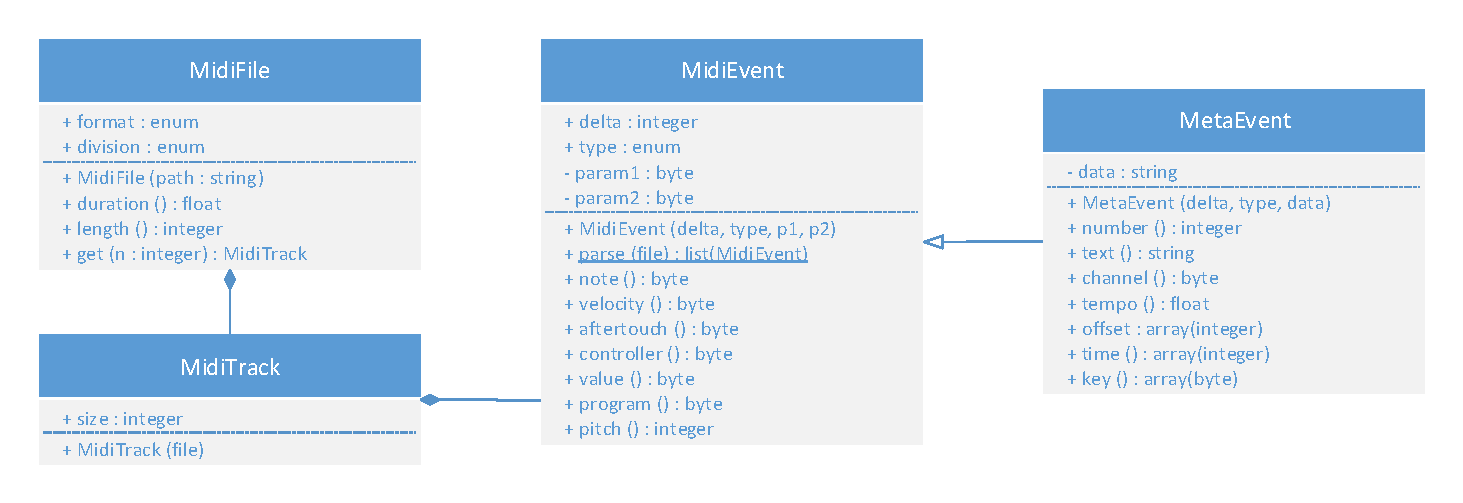
\includegraphics[width=0.75\textwidth]{images/uml_midi}
		\captionof{figure}{Diagrama de clases para el módulo MIDI.}
	\end{center}
	
	La implementación presentaba una \textbf{complejidad} notable, sobre todo porque no hay un carácter separador entre eventos, y tanto los meta-eventos como las marcas de duración tienen \textbf{longitud variable}. Además, hay que \textbf{intercambiar los \textit{bytes}} de los números que ocupen más de un \textit{byte}, para pasar de \textit{big-endian} a \textit{little-endian.}
	
	El \textbf{algoritmo de análisis} consiste en recorrer el archivo por \textbf{pistas}, y clasificar cada evento según su tipo.
	
	\begin{center}
		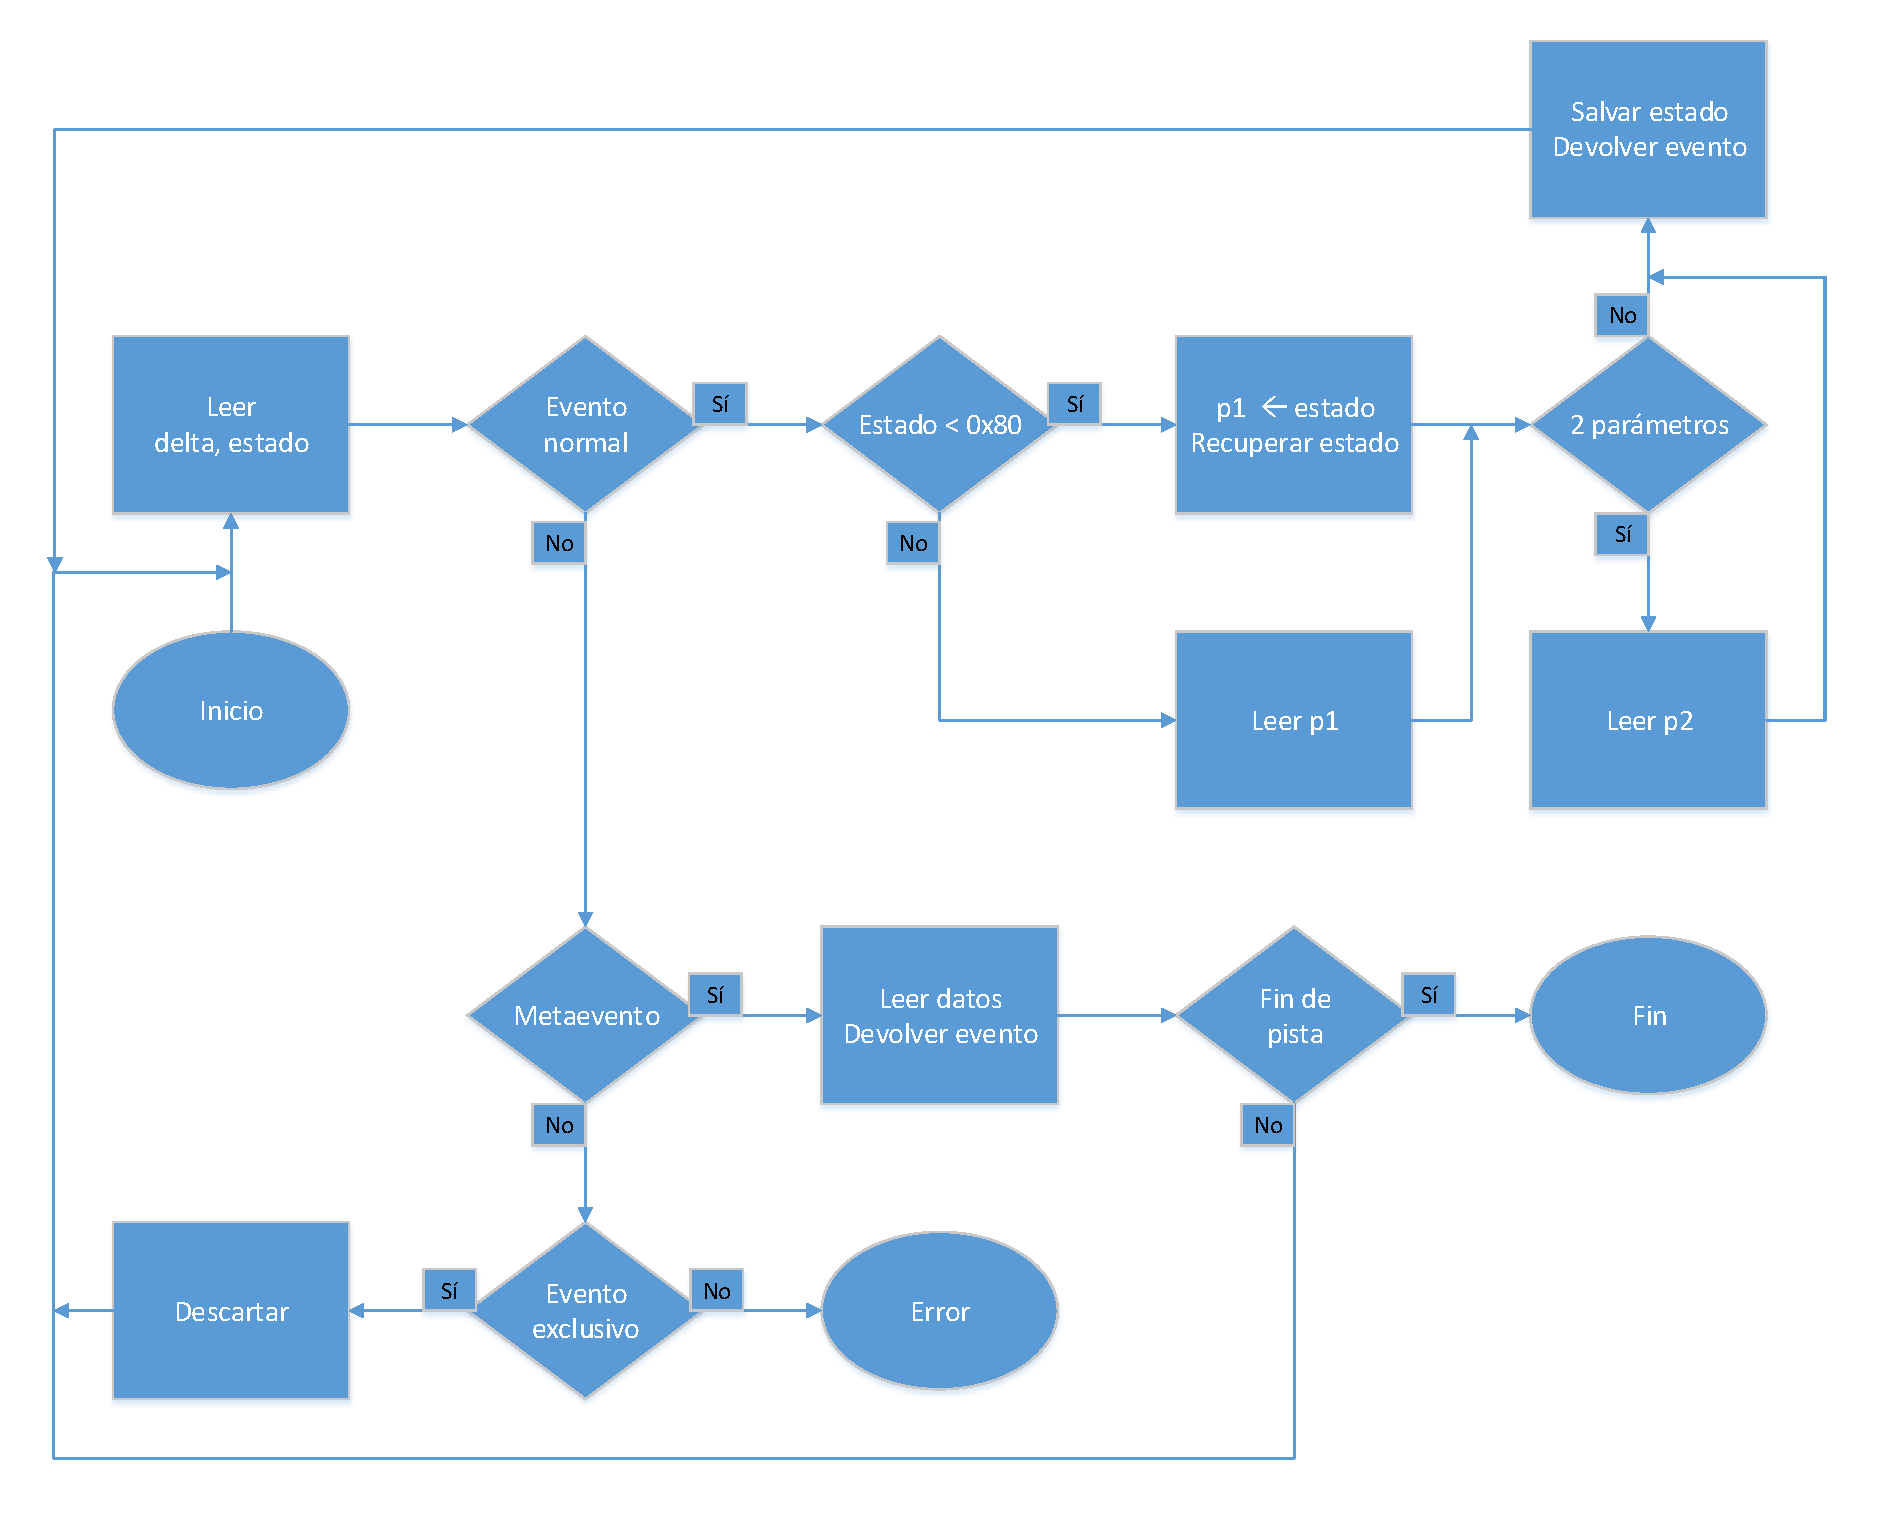
\includegraphics[width=0.75\textwidth]{images/flujo_parser}
		\captionof{figure}{Diagrama de flujo del analizador MIDI.}
	\end{center}
	
	En primer lugar hacemos una implementación sencilla en Python, que nos permita comprobar que hemos aplicado correctamente los conceptos. Una vez depurado, lo pasamos a C.
	
	\subsubsection*{Planificador}
	
	El planificador es la \textbf{pieza principal} del reproductor. Recibe las \textbf{órdenes} de los controladores y la lista de \textbf{partituras} a ejecutar. Una a una las lee con ayuda del módulo MIDI y \textbf{planifica los eventos} de todas las pistas para lanzarlos a la salida en el momento necesario.
	
	Utiliza una \textbf{hebra dinámica}, que podrá ser iniciada, pausada y detenida por el resto de procesos, por lo que hay que tener en cuenta los \textbf{problemas de concurrencia} para garantizar la \textbf{consistencia} del sistema.
	
	\begin{multicols}{2}
		\noindent
		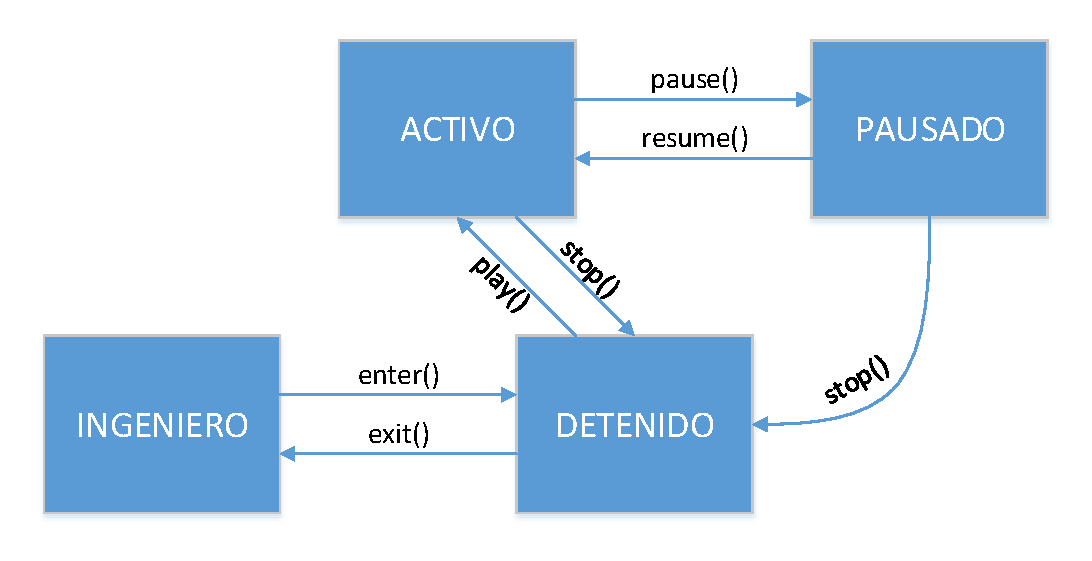
\includegraphics[width=0.45\textwidth]{images/estados} 
		\captionof{figure}{Diagrama de estados.}
		\columnbreak
		Para gestionar su funcionamiento, el planificador utiliza una pequeña \textbf{máquina de estados finitos}.
		
		Para evitar inconsistencias y condiciones de carrera, se utilizará un \textbf{mutex} que monitoriza las llamadas.
	\end{multicols}
	
	Un archivo MIDI está compuesto por varias pistas \textbf{simultáneas}. Ya que el procesador del \textit{Raspberry Pi} solo tiene un \textbf{núcleo}, no vamos a ganar tiempo designando una hebra para cada pista. Para que todas las pistas se ejecuten simultáneamente, diseñamos un \textbf{algoritmo inspirado en el \textit{merge sort}} que atienda a todas y decida qué evento debe ejecutarse en cada momento:
	
	El planificador recorre en cada ciclo todas las pistas, avanzando mientras sea el momento de ejecutar el evento correspondiente ($\Delta=0$). Cuando se ha llegado a un evento con $\Delta > 0$ en todas las pistas, se busca el \textbf{menor} de ellos y se resta al \textit{delta} de todos los eventos. A continuación, se solicita al sistema operativo la \textbf{espera} correspondiente al tiempo restado, y se repite el ciclo. El algoritmo \textbf{termina} cuando todas las pistas han llegado al final.
	
	\begin{center}
		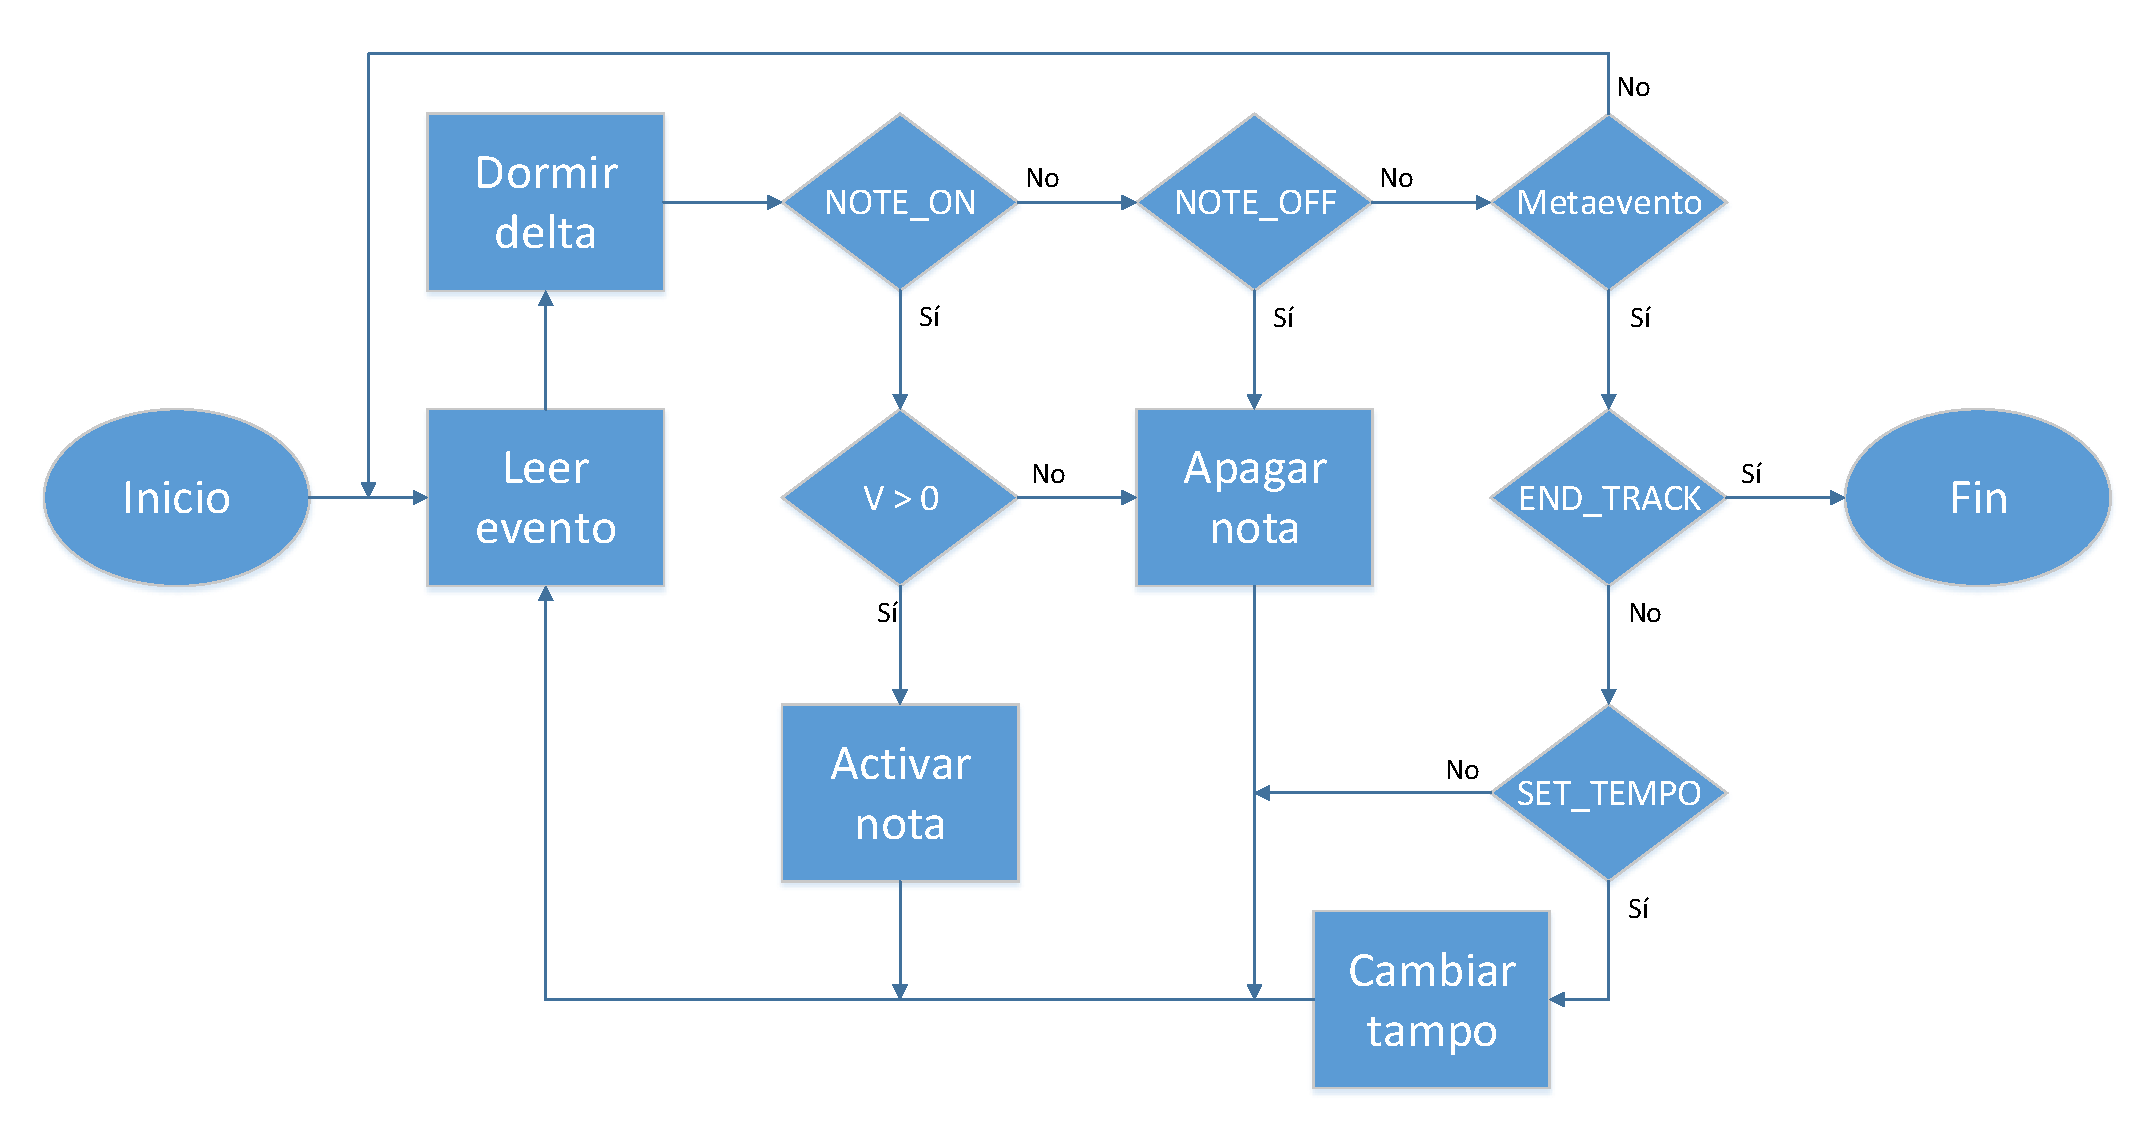
\includegraphics[width=0.75\textwidth]{images/flujo_planificacion} 
		\captionof{figure}{Diagrama de flujo del planificador (una pista).}
	\end{center}
	
	\subsubsection*{Salida hacia la PCB}
	
	Esta parte del programa supone el \textbf{puente} entre el planificador y la PCB, transformará instrucciones de activación y desactivación de notas en señales lógicas que emitiremos por el GPIO. 
	
	\clearpage
	
	El \textbf{reproductor} delega en el módulo de salida las siguientes funciones:
	
	\begin{enumerate}
		\item Dirigir las pistas de MIDI al canal de salida correspondiente.
		\item Almacenar el estado de salida (notas pulsadas y no pulsadas).
		\item Volcar la información en el GPIO.
		\item Hacer sonar el metrónomo.
	\end{enumerate}
	
	Éste será el único módulo que tendremos que cambiar a la hora de pasar de un órgano a otro. El hecho de \textbf{aislar la salida} también nos da flexibilidad para sustituir la interfaz GPIO por otro tipo de salida, como la consola, con fines de mantenimiento y depuración.
	
	\begin{multicols}{2}
		Nuestra especificación deja abierta la estructura que pueda tener un archivo MIDI. El sistema podrá descodificar MIDI estándar, pero la pieza deberá \textbf{adaptarse} a cada órgano concreto para lograr una óptima ejecución.
		
		El módulo de salida permitirá asignar cada pista MIDI, que normalmente corresponde a un \textbf{pentagrama} de la partitura, a un canal diferente.
		\columnbreak
		\begin{center}
			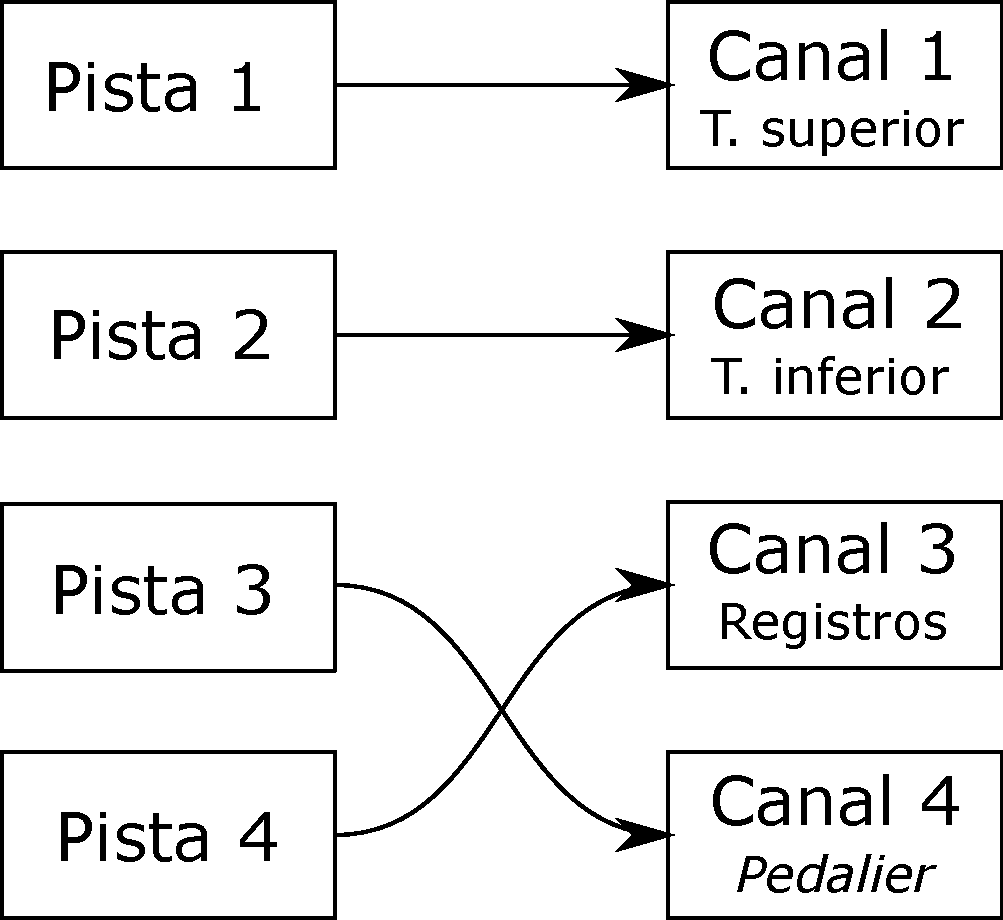
\includegraphics[width=0.45\textwidth]{images/map} 
			\captionof{figure}{Asignación de pistas.}
		\end{center}
	\end{multicols}
	
	\begin{multicols}{2}
		\noindent
		\begin{center}
			\begin{tabular}{|c|cccc|}
				\hline & \multicolumn{4}{c|}{N pistas} \\
				\hline \multirow{7}{*}{\rotatebox[]{90}{M notas}} & $s_{0,0}$ & $s_{0,1}$ & $s_{0,2}$ & $s_{0,3}$ \\
				& $s_{1,0}$ & $s_{1,1}$ & $s_{1,2}$ & $s_{1,3}$ \\
				& $s_{2,0}$ & $s_{2,1}$ & $s_{2,2}$ & $s_{2,3}$ \\
				& $s_{3,0}$ & $s_{3,1}$ & $s_{3,2}$ & $s_{3,3}$ \\
				& $s_{4,0}$ & $s_{4,1}$ & $s_{4,2}$ & $s_{4,3}$ \\
				& $s_{5,0}$ & $s_{5,1}$ & $s_{5,2}$ & $s_{5,3}$ \\
				& $s_{6,0}$ & $s_{6,1}$ & $s_{6,2}$ & $s_{6,3}$ \\
				\hline 
			\end{tabular}
			\captionof{table}{Notas en el estado.}
		\end{center}
		\columnbreak
		La \textbf{estructura de datos} que soportará el estado del órgano será conceptualmente una \textbf{matriz de bytes}, pero la implementaremos como un \textit{array}, que nos permita avanzar un puntero sobre él en el orden en que enviaremos la información hacia la PCB.
	\end{multicols}
	
	Para \textbf{acceder al GPIO}, durante la fase de prototipado utilizamos el sistema de archivos GPIO de Linux, pero en la implementación final utilizamos un método más eficiente: \textbf{mapeo en memoria} de la dirección física del periférico GPIO del BCM2835. Esto nos permite acceder a los pines desde un puntero y evitar hacer llamadas al sistema.
	
	Para \textbf{volcar el estado} en la PCB, seguimos el siguiente procedimiento:
	
	\begin{enumerate}
		\item \textbf{Escribir} el valor de una celda del vector en el puerto GPIO correspondiente.
		\item Emitir un \textbf{pulso} en el puerto conectado a SRCLK para \textbf{desplazar} y almacenar.
		\item Repetir los pasos 1 y 2 con el resto de \textit{bits}.
		\item Emitir un pulso en el puerto conectado a RCLK para \textbf{copiar} del registro de desplazamiento al registro de almacenamiento.
	\end{enumerate}
	
	Para \textbf{emitir un pulso} en el registro, actuamos de la siguiente forma, de acuerdo al manual técnico de los registros:
	
	\begin{enumerate}
		\item Escribir ''1'' en el puerto.
		\item Esperar 100 \textit{ns} con una llamada a \verb|sleep()|.
		\item Escribir ''0'' en el puerto.
	\end{enumerate}
	
	\subsubsection*{Control por socket}
	
	Un \textit{socket} es un mecanismo de \textbf{comunicación inter-proceso} que proporciona Linux para enviar y recibir datagramas en modo \textit{duplex}, bien dentro de la misma máquina (\textit{socket} local) o en una red (\textit{socket} de Internet).
	
	Vamos a crear un \textbf{\textit{socket} local}, accesible desde el sistema de archivos de Linux, que escuche peticiones de los clientes que se conecten, utilizando una interfaz basada en \textbf{lenguaje natural}, con un diseño sencillo y que mantenga la \textbf{coherencia} entre ambos subsistemas.
	
	Las peticiones que describen el protocolo resultante, así como las posibles respuestas, se enumeran de la siguiente forma:
	
	\begin{description}
		\item[PLAY <archivo> {[} <archivo>*{]}] Reproducir una lista de archivos MIDI. 
		
		\item[PLAYLOOP <archivo> {[} <archivo>* {]}] Reproducir en bucle una lista de archivos MIDI. 
		
		\item[PAUSE] Pausar la reproducción. Silencia las notas pero manteniendo el estado. 
		
		\item[RESUME] Reanuda la reproducción en el punto en que se pausó. 
		
		\item[STOP] Detiene completamente la reproducción y libera la lista de reproducción.
		
		\item[STATUS] Consulta el estado del reproductor. Respuesta:
		
		\begin{description}
			\item[PLAYING <archivo>] Reproduciendo el archivo especificado.
			\item[PAUSED <archivo>] Pausado en un punto del archivo indicado.
			\item[STOPPED] Detenido.
			\item[ENGINEER] En modo Ingeniería. No se podrá reproducir nada.
		\end{description}
	\end{description}
	
	\subsubsection*{Control del mando}
	
	el receptor del mando a distancia está conectado al \textit{Raspberry Pi} a través de los pines correspondientes al dispositivo \textbf{UART}, que controla los puertos serie.
	
	Este módulo tiene una topología análoga al control por \textit{socket}, tan solo cambia el origen y la forma de entrada de los datos. Establecerá una comunicación con el puerto serie e iniciará un \textbf{bucle de escucha}. La sintaxis del mensaje, como ya sabemos, es:
	
	\begin{center}
		<Nº serie (7 \textit{bytes})> <Botón (1 \textit{byte})> <CRLF>
	\end{center}
	
	De esta forma, el servicio tan solo debe \textbf{verificar el nº de serie} y \textbf{ejecutar} la orden correspondiente, según el siguiente esquema:
	
	\begin{description}
		\item[Botón 1] Inicia la lista de reproducción asignada al botón 1.
		\item[Botón 2] Reproduce la lista asignada al botón 2.
		\item[Ambos] Pausa la reproducción, o la reanuda.
	\end{description}
	
	Además de reconocer la pulsación del mando, es necesario consultar en la \textbf{base de datos} la lista que corresponde al botón pulsado y los archivos contenidos, que serán transmitidos al planificador.
	
	\subsubsection*{Comunicación con la base de datos}
	
	La información relativa a la lista de reproducción asignada a un botón, así como la lista de partituras correspondientes, residirán en una base de datos, que definiremos en la sección \ref{subsec:database}. Así, enmarcaremos un nuevo módulo dedicado a \textbf{consultar} la información requerida, ofreciendo una \textbf{interfaz independiente} del sistema de gestión de bases de datos que utilicemos, y de la propia base de datos.
	
	Utilizaremos \textbf{MySQL}, de forma que nuestro módulo utilizará la biblioteca cliente de MySQL para C.
	
	\subsubsection*{Modo Ingeniería}
	
	El sistema requiere un modo de mantenimiento para regular la \textbf{mecánica}, al que se accederá localmente, a través de una interfaz reducida que controlaremos con el codificador rotatorio y el LCD. Este sistema permitirá controlar las siguientes acciones:
	
	\begin{enumerate}
		\item Entrar en modo Ingeniería.
		\item Activar y desactivar el metrónomo.
		\item Apagar y reiniciar el sistema.
	\end{enumerate}
	
	El codificador permitirá acceder al \textbf{modo Ingeniería}, que detendrá la reproducción ---si estaba en funcionamiento--- y  aislará el planificador, ganando acceso directo a la salida GPIO. Funcionará en una hebra independiente.
	
	Vamos a diseñar la interfaz como una \textbf{máquina de estados}: Inicialmente el modo Ingeniería está desactivado, girando el botón se nos dará la opción de activarlo, y al pulsarlo entraremos en él. Se activará la nota más baja de la primera pista, al girar el botón podremos movernos cíclicamente por todas las notas de esa pista. Pulsando el botón cambiamos a la segunda pista, luego a la tercera, y así hasta la última. Si apretamos nuevamente el botón, volvemos al menú que nos permitirá salir del modo Ingeniería.
	
	También vamos a insertar en el menú opciones para habilitar el \textbf{metrónomo} y para \textbf{desactivar el sistema}. Este diagrama muestra las \textbf{transiciones} entre los estados:
	
	\begin{center}
		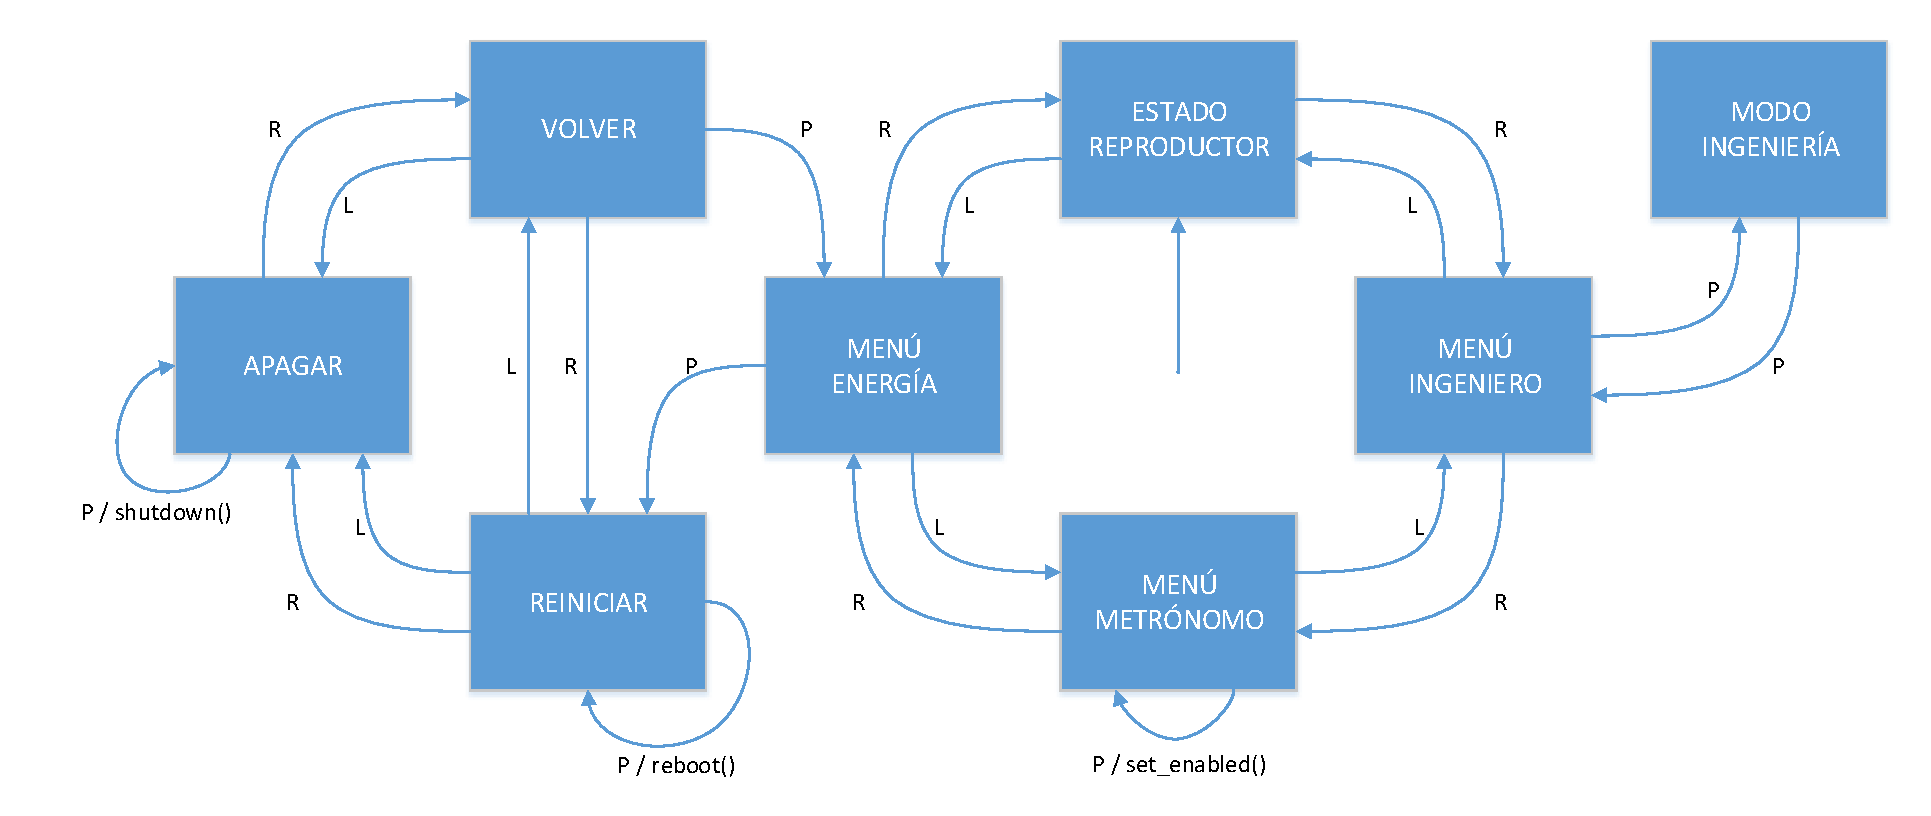
\includegraphics[width=0.75\textwidth]{images/engineer} 
		\captionof{figure}{Máquina de estados del modo Ingeniería.}
	\end{center}
	
	\subsubsection*{Seguridad}
	
	Es muy importante que el demonio se mantenga en funcionamiento y con \textbf{capacidad de respuesta}. Para ello, puliremos toda la programación relativa a la \textbf{entrada de datos}.
	
	El \textbf{desbordamiento de memoria} de entrada ---\textit{buffer overflow}--- se produce cuando una función de lectura acepta una cadena \textbf{mayor que la memoria} que tenía reservada. Este riesgo podría producir una \textbf{violación de segmento} o incluso ser aprovechado por un \textbf{intruso} para modificar las instrucciones del programa, accediendo ilegalmente al sistema.
	
	La \textbf{solución} adoptada es utilizar una cantidad razonable de memoria y limitar la cadena de entrada acotando tanto la \textbf{recepción} de datos desde el \textit{socket} como la \textbf{comparación} de cadenas.
	
	Otra capa de seguridad se implanta utilizando \textbf{permisos de usuario} en el sistema de archivos de Linux: creamos el usuario \verb|organ| y su grupo correspondiente, que serán \textbf{dueños} del proceso demonio y del \textit{socket}. Solo los usuarios autorizados (pertenecientes al grupo \verb|organ|) podrán utilizar el \textit{socket}.
	
	Por último, respecto a la \textbf{concurrencia}, protegeremos todas las funciones públicas del planificador para evitar inconsistencias o \textbf{condiciones de carrera}, ya que se puede llamar desde varias hebras.
	
	\subsection{Interfaz web}
	
	El próximo paso es \textbf{concebir el \textit{front-end}} que, a tenor de los requisitos que propusimos al inicio, ofrezca al usuario la interfaz más completa posible. Frecuentemente la \textbf{funcionalidad} viene contrapuesta a la \textbf{facilidad} de uso; es nuestra tarea encontrar el mejor \textbf{equilibrio} posible.
	
	Vamos a diseñar una solución enfocada al uso remoto con ayuda de un \textbf{explorador} de Internet, como \textit{Chrome}, \textit{Firefox} o \textit{Safari}, con lo que crearemos un servidor \textit{web}.
	
	\begin{multicols}{2}
		Para estructurar los elementos que conformarán la interfaz, utilizaremos el patrón de \textbf{modelo-vista-controlador}.
		
		Considerando los casos de uso y los requisitos, hemos enmarcado en el esquema estos elementos:
		\columnbreak
		\begin{center}
			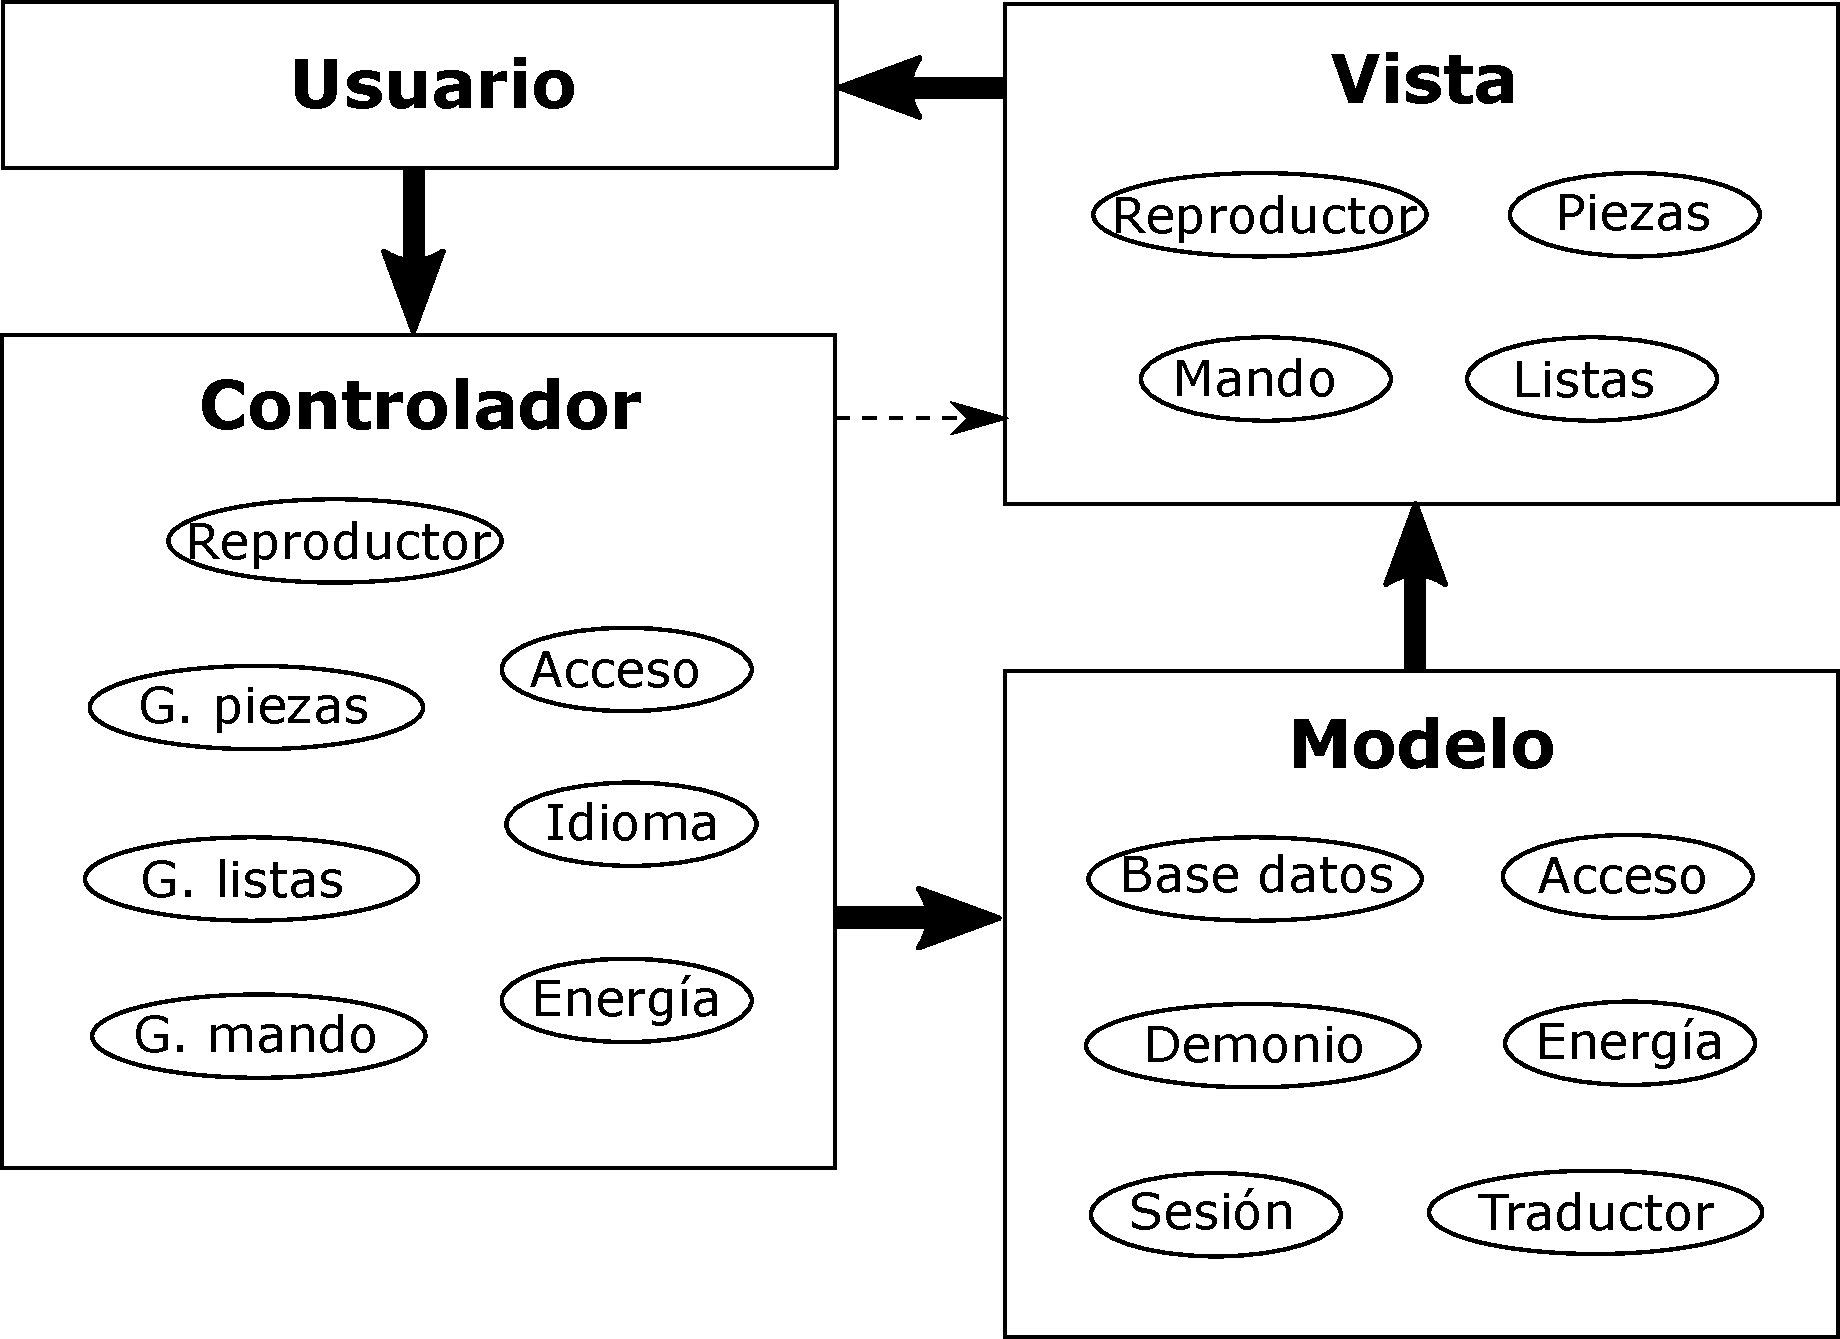
\includegraphics[width=0.45\textwidth]{images/mvc_completo} 
			\captionof{figure}{Componentes del sistema.}
		\end{center}
	\end{multicols}
	
	Usaremos las siguientes \textbf{tecnologías}:
	
	\begin{enumerate}
		\item PHP 5.4, como lenguaje de programación.
		\item HTML 5, como lenguaje de marcado.
		\item CSS 3, para las hojas de estilos.
		\item XML, para almacenar información estática.
		\item JavaScript, AJAX y DOM, para interactuar dinámicamente con la página.
	\end{enumerate}
	
	\subsubsection*{Portada}
	
	La portada es la vista principal y va a cumplir estas funciones:
	
	\begin{enumerate}
		\item Presentar la aplicación y dar la bienvenida.
		\item Introducir una contraseña para acceder al sistema.
		\item Informar de un apagado o un reinicio.
		\item Alertar de que la contraseña no es válida.
	\end{enumerate}
	
	El módulo de autentificación recibe la \textbf{contraseña} introducida por el usuario, y utiliza la interfaz del modelo para validarla. La contraseña será la de un usuario (a especificar) del sistema \textbf{Linux}, que provee una forma segura de almacenar contraseñas cifradas y gestionar usuarios.
	
	\begin{multicols}{2}
		\noindent
		\begin{center}
			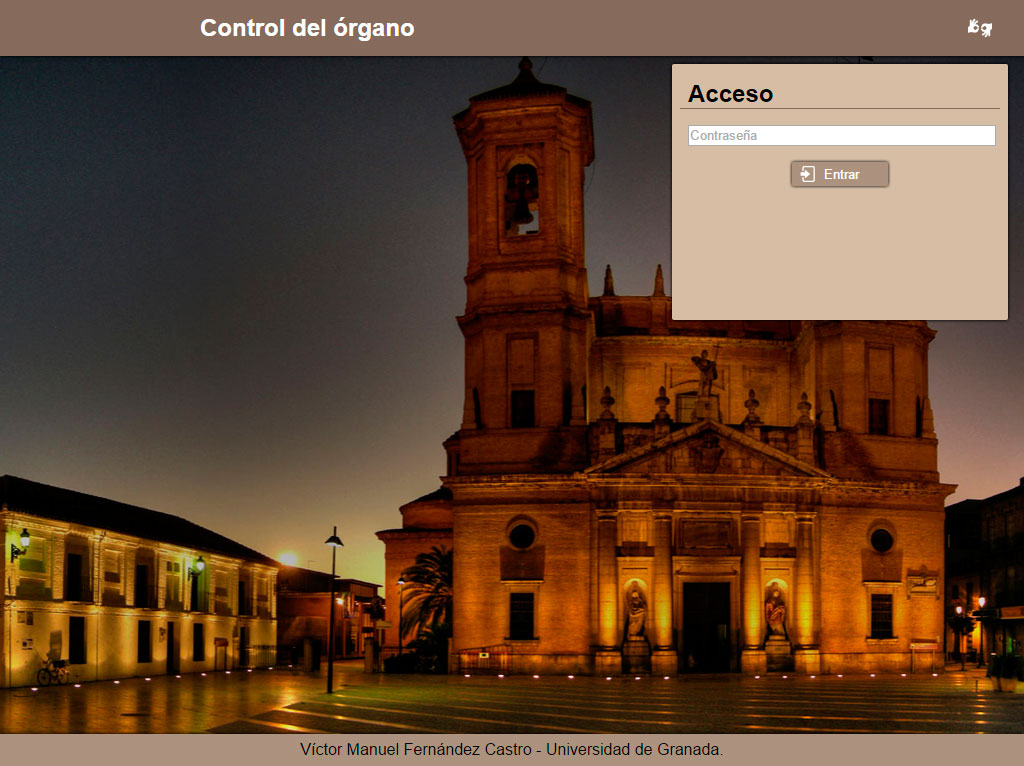
\includegraphics[width=0.45\textwidth]{images/cap_portada} 
			\captionof{figure}{Vista de la portada.}
		\end{center}
		\columnbreak
		La vista proporcionará un fondo dinámico, con varias \textbf{imágenes temáticas}, y un cuadro para introducir la contraseña. 
		
		Al hacerlo, se enviará al controlador, que se ocupará de \textbf{verificar} que la clave es correcta y concederá el acceso al reproductor.
	\end{multicols}
	
	Por razones de seguridad, la utilidad de autentificación \textbf{retrasa} la ejecución 2 segundos en caso de recibir una contraseña incorrecta, atenuando la efectividad de un \textbf{ataque por fuerza bruta}.
	
	\subsubsection*{Reproductor}
	
	\begin{multicols}{2}
		\noindent
		\begin{center}
			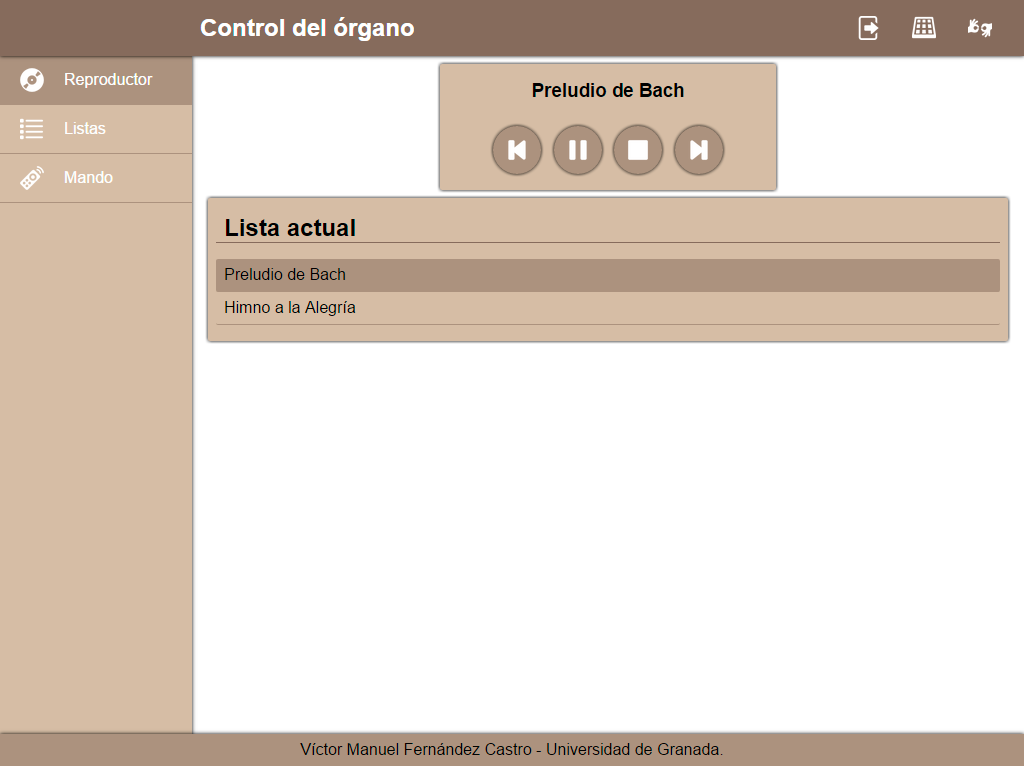
\includegraphics[width=0.45\textwidth]{images/cap_reproductor} 
			\captionof{figure}{Vista del reproductor.}
		\end{center}
		\columnbreak
		Ésta es la página principal del administrador, desde la que podremos controlar la reproducción del órgano. Tendrá la funcionalidad básica de cualquier reproductor.
		
		Guiados por la lista de controles requeridos y la filosofía de \textit{Material Design}, proponemos esta interfaz visual.
	\end{multicols}
	
	El protocolo de comunicación establece que el reproductor del demonio no es consciente de la lista de reproducción en la base de datos. Al solicitar una reproducción se le envía los \textbf{nombres de archivo}. De igual forma, al consultar el estado, devuelve el nombre de la pieza que se está ejecutando, cuya lista se puede conocer por \textbf{reunión natural} en la base de datos.
	
	Esto se hace así para evitar mantener un \textbf{estado común} entre el demonio y la interfaz, que podría provocar \textbf{incoherencias} si el cliente se desconecta repentinamente o si hay varios usuarios conectados al mismo tiempo.
	
	\subsubsection*{Gestión de partituras y listas}
	
	Esta parte de la aplicación nos permite administrar las piezas almacenadas en el sistema, crear y modificar listas de reproducción, y gestionar las partituras que contienen.
	
	El módulo consta de \textbf{dos vistas}: una para ver las \textbf{listas} existente y crear nuevas, y otra para gestionar las \textbf{piezas} contenidas en cada lista, a la que accedemos desde la primera página.
	
	\begin{multicols}{2}
		\noindent
		\begin{center}
			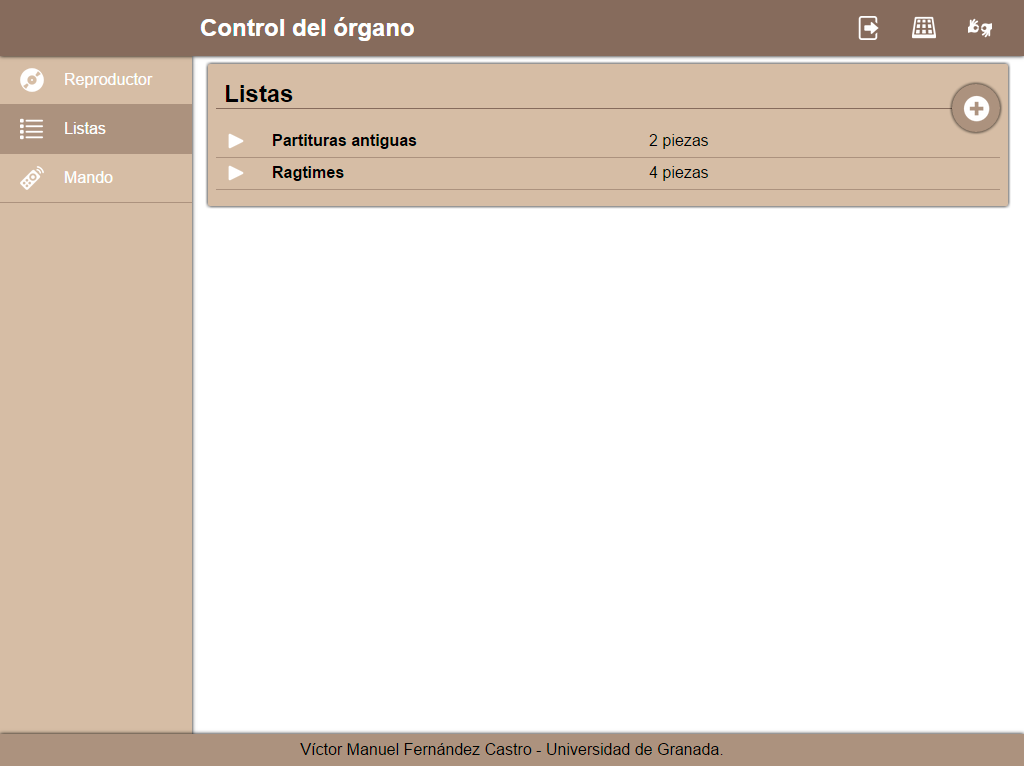
\includegraphics[width=0.45\textwidth]{images/cap_listas} 
			\captionof{figure}{Vista del gestor de listas.}
		\end{center}
		\columnbreak
		El gestor de listas consiste esencialmente en una \textbf{tabla} que muestra las listas que hemos creado, nos da a conocer el nombre y el número de piezas contenidas. 
		
		Además proporciona un botón para \textbf{reproducir} directamente la lista. La página muestra también un botón para \textbf{insertar} una lista nueva.
	\end{multicols}
	
	Para \textbf{crear una lista}, el botón correspondiente llama a una función JavaScript, que hace aparecer una \textbf{ventana modal} con un pequeño formulario para que introduzcamos el nombre de la nueva lista.
	
	Por \textbf{seguridad}, el campo es obligatorio y está limitado a 255 caracteres, la misma longitud que la columna de la base de datos que almacenará esta información. Aún así, el \textbf{controlador} realizará una segunda comprobación cuando reciba los datos.
	
	\begin{multicols}{2}
		\noindent
		\begin{center}
			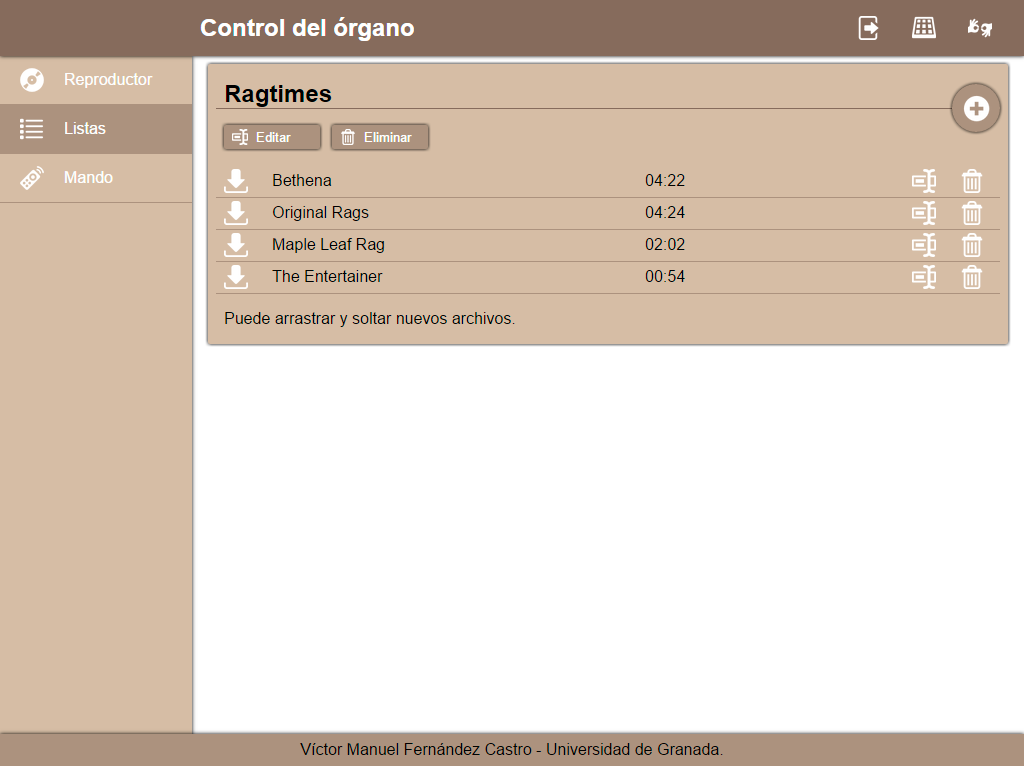
\includegraphics[width=0.45\textwidth]{images/cap_piezas} 
			\captionof{figure}{Vista del gestor de piezas.}
		\end{center}
		\columnbreak
		El gestor de partituras está estrechamente relacionado con el de listas de reproducción, en tanto que realmente es el \textbf{gestor de una lista} concreta. 
		
		Desde aquí podremos conocer el contenido de cada lista, así como renombrarla y eliminarla. Al mismo tiempo, servirá para añadir \textbf{partituras}, cambiar su título y borrarlas, de una forma similar a las propias listas.
	\end{multicols}
	
	Hay \textbf{dos métodos} para subir archivos, aunque ambos llaman a la misma función del controlador:
	
	\begin{enumerate}
		\item Seleccionando un archivo MIDI en el explorador que aparece al pulsar el\textbf{ botón para añadir} una pieza. El archivo se envía en el formulario de manera normal. Solo se permite seleccionar un fichero y, de fallar, recibiremos un mensaje de error indicando los motivos.
		
		\item \textbf{Arrastrando} uno o varios archivos a la sección central de la vista. Al hacerlo, aparecerá un \textbf{panel modal} que indicará el archivo que se está enviando. Si un archivo falla, es descartado silenciosamente.
	\end{enumerate}
	
	\clearpage
	\subsubsection*{Asignación del mando}
	
	Una vez creadas las listas, tendremos la posibilidad de asignarlas a un botón del mando a distancia. La \textbf{base de datos} almacena esta información y permite que sea consultada directamente por el demonio, que será el que reciba las pulsaciones del mando.
	
	\begin{multicols}{2}
		\noindent
		\begin{center}
			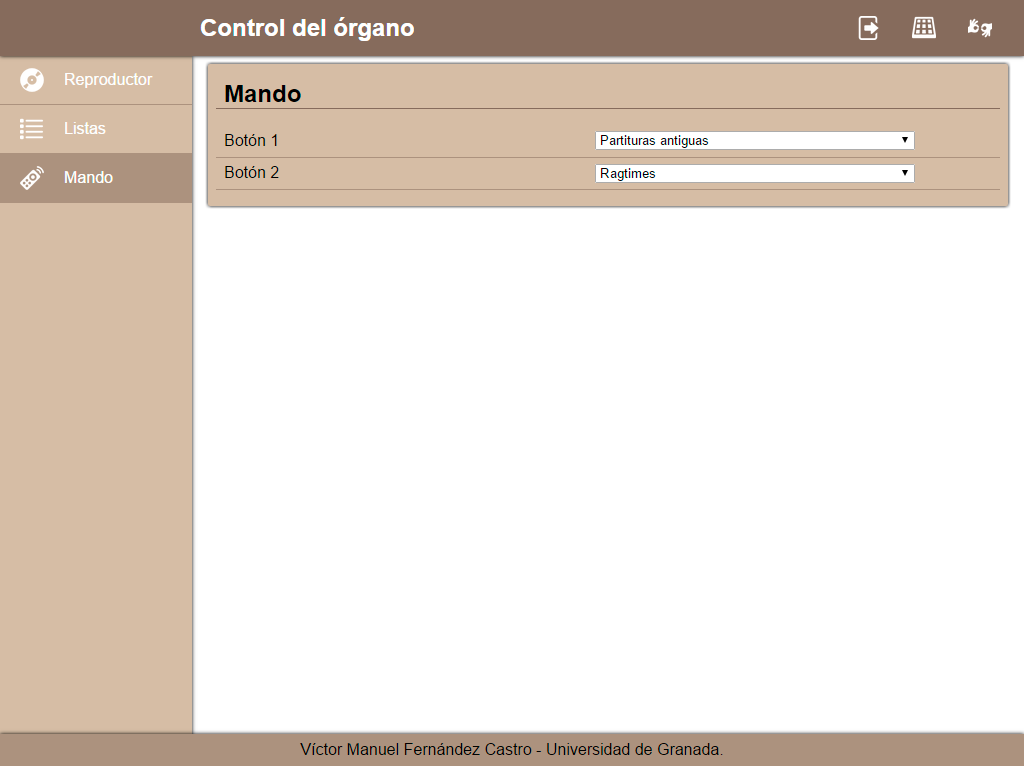
\includegraphics[width=0.45\textwidth]{images/cap_mando} 
			\captionof{figure}{Vista del gestor del mando.}
		\end{center}
		\columnbreak
		El gestor de partituras está estrechamente relacionado con el de listas de reproducción, en tanto que realmente es el \textbf{gestor de una lista} concreta. 
		
		Desde aquí podremos conocer el contenido de cada lista, así como renombrarla y eliminarla. Al mismo tiempo, servirá para añadir \textbf{partituras}, cambiar su título y borrarlas, de una forma similar a las propias listas.
	\end{multicols}
	
	\subsubsection*{Energía y multilenguaje}
	
	Hemos contemplado proveer la posibilidad de\textbf{ apagar o reiniciar el sistema} remotamente. Para ello, ofreceremos un menú en la cabecera de la pantalla, que será común a todas las vistas, excepto la portada, con opciones para apagar y reiniciar el sistema.
	
	\begin{center}
		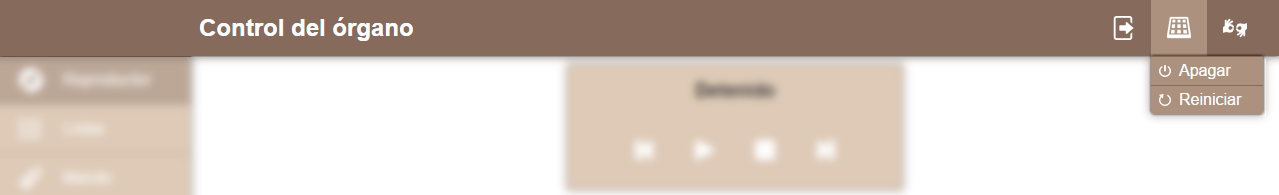
\includegraphics[width=0.75\textwidth]{images/cap_repr_apagar} 
		\captionof{figure}{Menú de control de energía.}
	\end{center}
	
	Uno de los requisitos especificados es que la interfaz \textbf{soporte varios idiomas}. Modelaremos la solución para que sea fácil tanto escoger un idioma como \textbf{agregar} nuevas lenguas.
	
	Para ello, utilizaremos \textbf{archivos de traducción} independientes que el sistema detectará automáticamente, permitiendo que añadir un idioma sea tan sencillo como agregar un fichero nuevo.
	
	Al igual que el control de energía, el selector de idioma aparecerá como un menú desplegable en la \textbf{cabecera} de la aplicación, pero a diferencia de aquél, también se mostrará en la portada.
	
	\begin{center}
		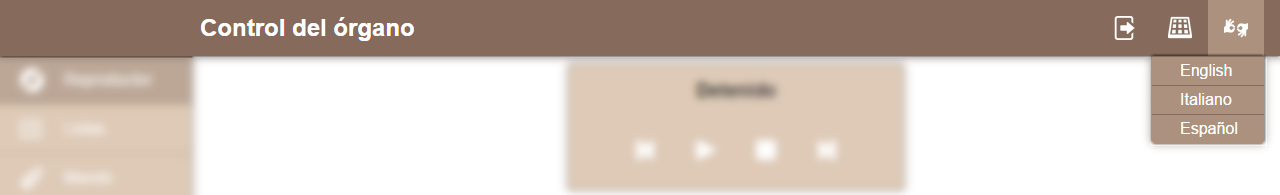
\includegraphics[width=0.75\textwidth]{images/cap_repr_idiomas} 
		\captionof{figure}{Menú de selección de idioma.}
	\end{center}
	
	\subsubsection*{Seguridad}

	En el \textit{front-end} implantaremos dos capas de seguridad:
	
	\begin{enumerate}
		\item Una primera capa en la \textbf{vista}, para informar inmediatamente de un error en un formulario.
		\item Otra capa en el \textbf{controlador}, para evitar errores más complejos o un conjunto de datos forzado.
	\end{enumerate}
	
	Siguiendo este método, la longitud de los \textbf{campos de texto} de los formularios están limitados tanto en la vista como en el controlador.
	
	Para evitar añadir archivos que no sean de \textbf{formato MIDI}, el controlador del gestor de piezas llama al \textit{analizador de MIDI} antes de insertar el fichero.
	
	Todas las cadenas dirigidas a hacer una consulta en la base de datos pasan por un \textbf{filtrado} para evitar la \textbf{inyección de código}. También se filtrará la contraseña de usuario, ya que se envía a una orden de Linux y podría comprometer la seguridad del sistema.
	
	Como medida adicional, las \textbf{credenciales} de usuario cedidas a la aplicación PHP para acceder a la base de datos solo tienen permisos para alterar el \textbf{contenido} de las tablas, no para modificar las propias tablas.
	
	Por último, tal como mencionamos anteriormente, el usuario del servidor Apache, \verb|www-data|, debe pertenecer al grupo \verb|organ| para poder comunicarse con el demonio a través del \textit{socket}.
	
	\subsection{Base de datos}
	\label{subsec:database}
	
	La información que queremos almacenar funciona de la siguiente forma:
	
	\begin{enumerate}
		\item Las \textbf{partituras} se guardan en un archivo, cuyo nombre no tiene que coincidir con el título de la partitura.
		\item De una partitura podremos conocer su \textbf{duración}.
		\item Una \textbf{lista de reproducción} es una colección de partituras, y le asignaremos un nombre.
		\item Cada partitura pertenecerá a una lista de reproducción, y solo a una.
		\item Un \textbf{botón} se distingue por su código, y se le asigna a una lista de reproducción, sin perjuicio de que una lista esté asignada a varios botones. Naturalmente, puede haber listas que no estén asignadas a ningún botón.
	\end{enumerate}
	
	\clearpage
	
	\begin{multicols}{2}
		\noindent
		\begin{center}
			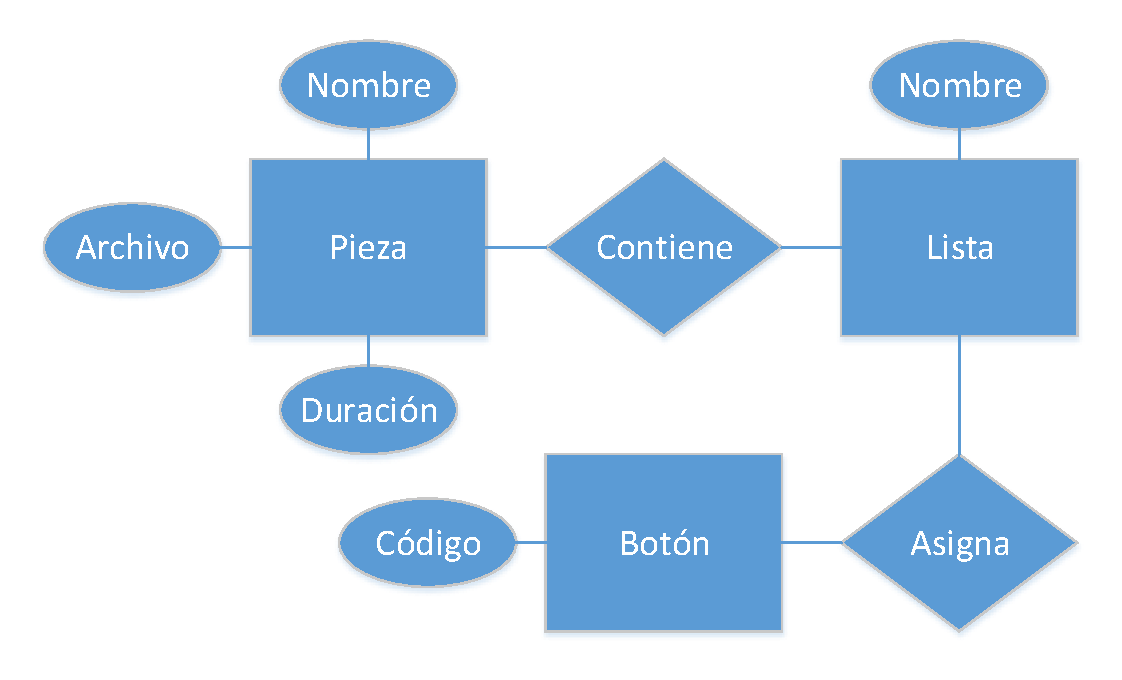
\includegraphics[width=0.45\textwidth]{images/bd_er} 
			\captionof{figure}{Modelo entidad-relación.}
		\end{center}
		\columnbreak
		Una vez hemos considerado las entidades, sus atributos y las relaciones, diseñamos el \textbf{modelo de datos}, que depende del tipo de sistema de gestión de bases de datos que vayamos a utilizar.
		
		En nuestro caso, utilizaremos un \textbf{DBMS relacional}.
	\end{multicols}
	
	Una vez hemos considerado las entidades, sus atributos y las relaciones, diseñamos el \textbf{modelo de datos}, que depende del tipo de sistema de gestión de bases de datos que vayamos a utilizar. En nuestro caso, utilizaremos un \textbf{DBMS relacional}.
	
	Hemos escogido \textbf{MySQL}, ya que su motor InnoDB soporta transacciones ACID e integridad referencial. Además, gestiona de manera eficiente los accesos concurrentes.
	
	\begin{center}
		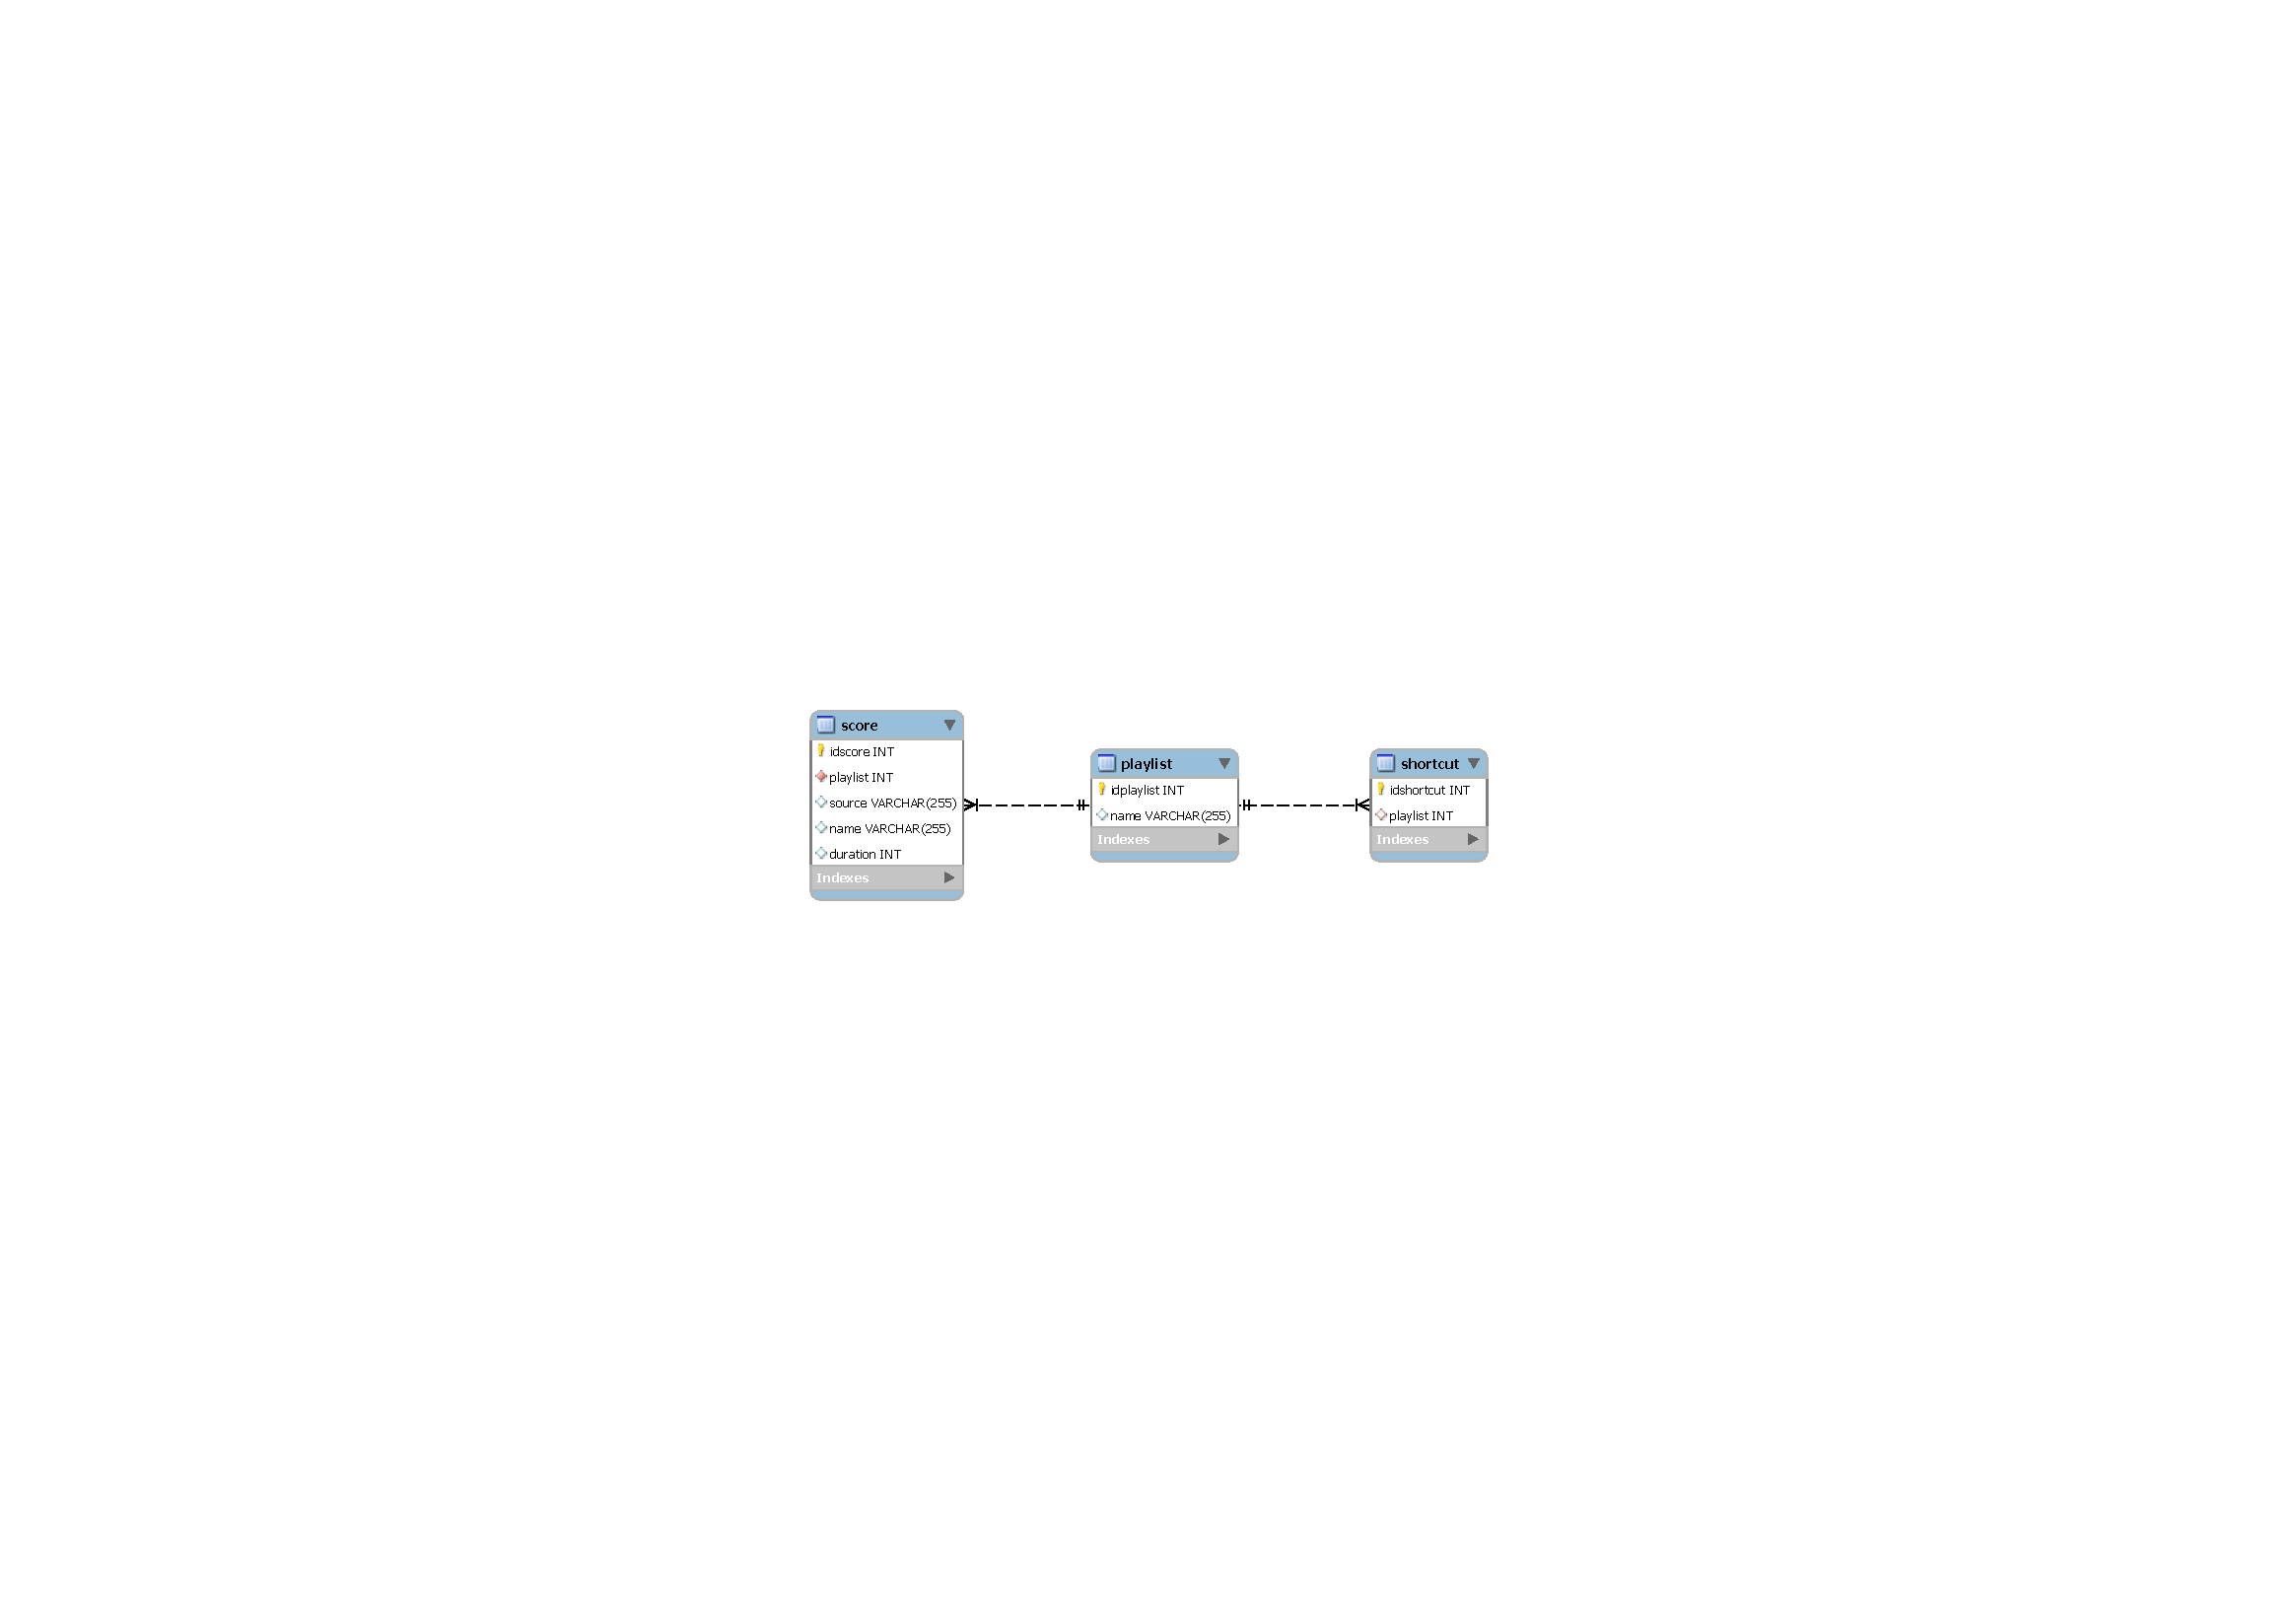
\includegraphics[width=0.75\textwidth]{images/bd_rel} 
		\captionof{figure}{Modelo relacional de MySQL.}
	\end{center}
	
	Para garantizar que la base de datos mantendrá la información coherente y sin anomalías, estudiamos las relaciones para \textbf{normalizarlas}. Hemos hecho el diseño de la base de datos en \textbf{5ª forma normal}.
	
	\subsection{Aplicaciones auxiliares}
	
	Existe una \textbf{dependencia mutua} total entre los bloques que componen nuestro sistema, contraproducente para la fase de implementación, donde será necesario realizar \textbf{pequeñas pruebas} sobre el código que vayamos construyendo.
	
	Para \textbf{verificar el desarrollo}, vamos a prever la necesidad de probar los módulos críticos del diseño:
	
	\begin{multicols}{2}
		\begin{enumerate}[nosep,itemsep=1em]
			\item Descodificador de archivos MIDI.
			\item Planificador.
			\item Interfaz de salida.
			\item Servidor \textit{socket}.
		\end{enumerate}
		\columnbreak
		\begin{center}
			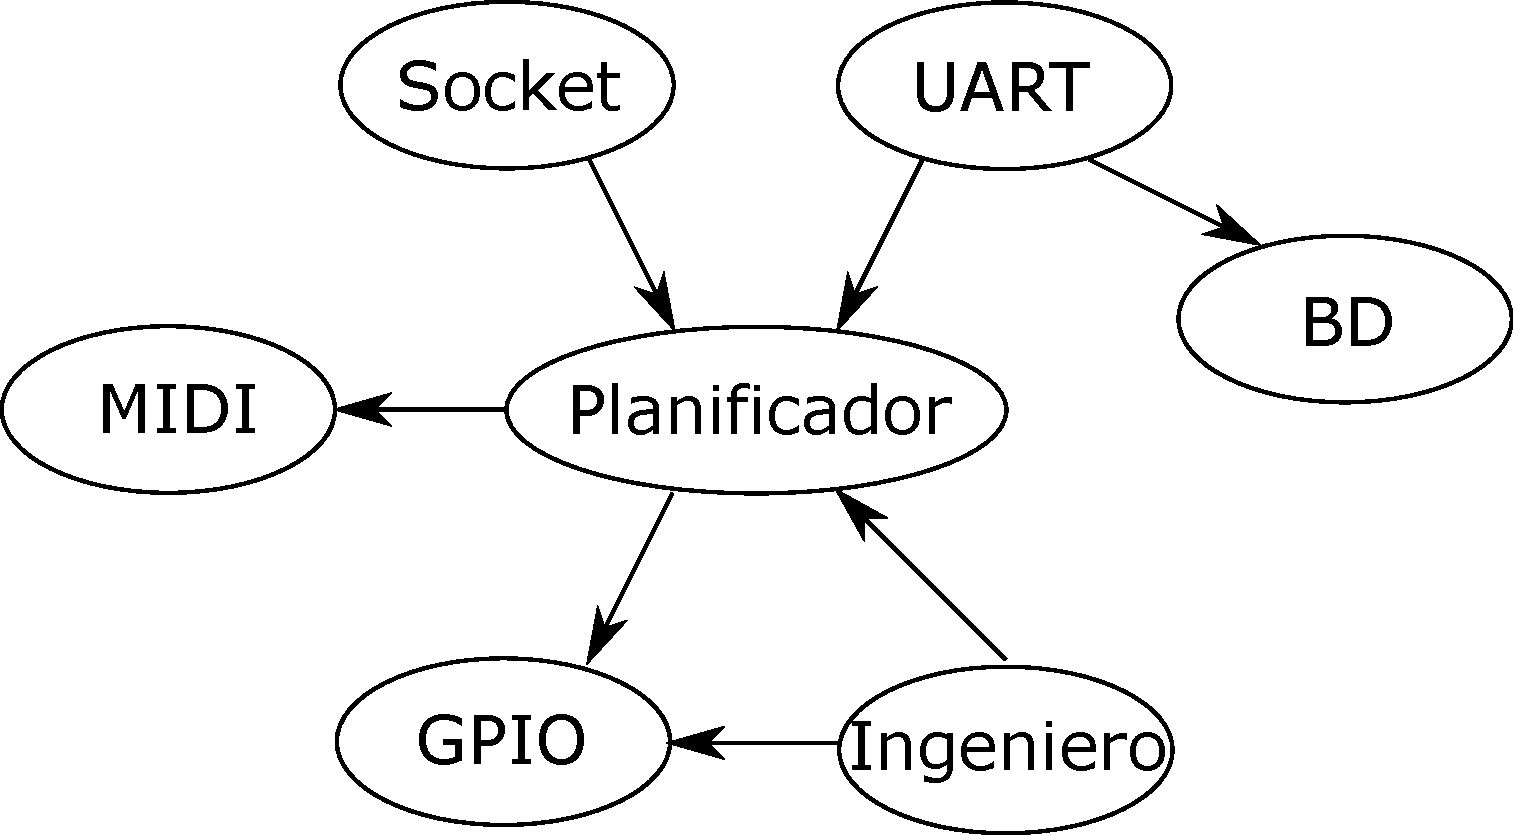
\includegraphics[width=0.45\textwidth]{images/daemon} 
			\captionof{figure}{Componentes del back-end.}
		\end{center}
	\end{multicols}
	
	Por otro lado, el \textit{front-end} necesita dos aplicaciones externas para distintos fines:
	
	\begin{enumerate}
		\item El gestor de piezas requiere \textbf{validar} y conocer la \textbf{duración} de una partitura mediante un programa que analice archivos MIDI.
		
		\item El componente de autentificación necesita comprobar externamente la \textbf{contraseña} introducida por el usuario.
	\end{enumerate}
	
	\subsubsection*{Información de archivo MIDI}
	
	Esta aplicación cumplirá dos fines:
	
	\begin{enumerate}
		\item Validar el analizador de archivos MIDI.
		\item Servir al \textit{front-end} la duración de una partitura.
	\end{enumerate}
	
	Sencillamente, utilizará la interfaz de programación creada por el descodificador MIDI para enviar el nombre de un fichero, \textbf{descodificarlo} y mostrar en la salida estándar la información básica de una partitura:
	
	\begin{multicols}{2}
		\begin{enumerate}
			\item Organización de las pistas.
			\item Número de pistas.
			\item División de tiempo.
			\item Duración de la obra.
		\end{enumerate}
		\columnbreak
		\begin{center}
			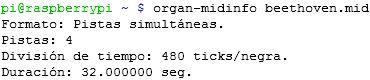
\includegraphics[width=0.45\textwidth]{images/cap_midinfo} 
			\captionof{figure}{Información de MIDI.}
		\end{center}
	\end{multicols}
		
	\subsubsection*{Simulador de reproducción}
	
	Vamos a hacer una pequeña aplicación que nos permita verificar el funcionamiento del planificador y la interfaz de salida, de la siguiente manera:
	
	\begin{enumerate}
		\item Interactuará directamente con el planificador, de la misma forma que hará el \textit{socket} o el UART.
		\item Implementará la salida (diseñada para el GPIO) sobre la salida estándar, suplantando a la PCB.
	\end{enumerate}
	
	En este caso vamos a simular más exactamente el órgano de la Parroquia de la Encarnación de Santa Fe que el prototipo de la PCB, en tanto que ésta solo abordará 7 notas en cada canal. En resumen tendremos esta estructura:
	
	\begin{center}
		\begin{tabular}{|l|l|l|l|}
			\hline \textbf{Pista} & \textbf{Extensión} & \textbf{Comienzo} & \textbf{Descripción} \\ 
			\hline 1 & 49 notas & 36 (\textit{Do-2}) & Teclado barroco \\
			\hline 2 & 49 notas & 36 (\textit{Do-2}) & Teclado romántico \\
			\hline 2 & 12 notas & 36 (\textit{Do-1}) & Pedalier \\
			\hline 2 & 49 notas & 36 (\textit{Do-4}) & Registros \\
			\hline 
		\end{tabular}
		\captionof{table}{Asignación de notas en el simulador de reproducción.}
	\end{center}
	
	\subsubsection*{Terminal del reproductor}
	
	Una vez implementados los componentes críticos del demonio, crearemos un sencillo programa que haga las \textbf{llamadas básicas} del protocolo a través del \textit{socket}, como lo hará la interfaz gráfica. Esto nos permitirá comprobar que la estructura principal funciona correctamente, y \textbf{manejar el reproductor} sin la interfaz gráfica.
	
	La aplicación admitirá los siguientes argumentos:
	
	\begin{center}
		\verb!organ play[loop] <archivo> | pause | resume | stop | status !
	\end{center}
	
	\subsubsection*{Comprobación de contraseña}
	
	Por último, concebiremos una aplicación minimalista para comprobar la contraseña del usuario. Este programa será llamado por el servidor \textit{web} cuando un usuario intente acceder a la interfaz.
	
	La aplicación recibe los siguientes argumentos por consola:
	
	\begin{enumerate}
		\item Nombre de usuario.
		\item Contraseña introducida.
	\end{enumerate}
	
	Se verificará que la contraseña introducida corresponda a la del \textbf{usuario en Linux} con el nombre indicado, y el resultado se indicará como código de salida del proceso: 0 en caso de éxito, o 1 en caso de error.
	
	\subsection{Resultado}
	
	La fase de diseño nos ha permitido afinar con un alto nivel de detalle el esbozo inicial, hasta obtener los tres grandes bloques del sistema. En definitiva, hemos concebido un completo sistema de control para la PCB, cuyo funcionamiento se resume en el siguiente diagrama:
	
	\begin{center}
		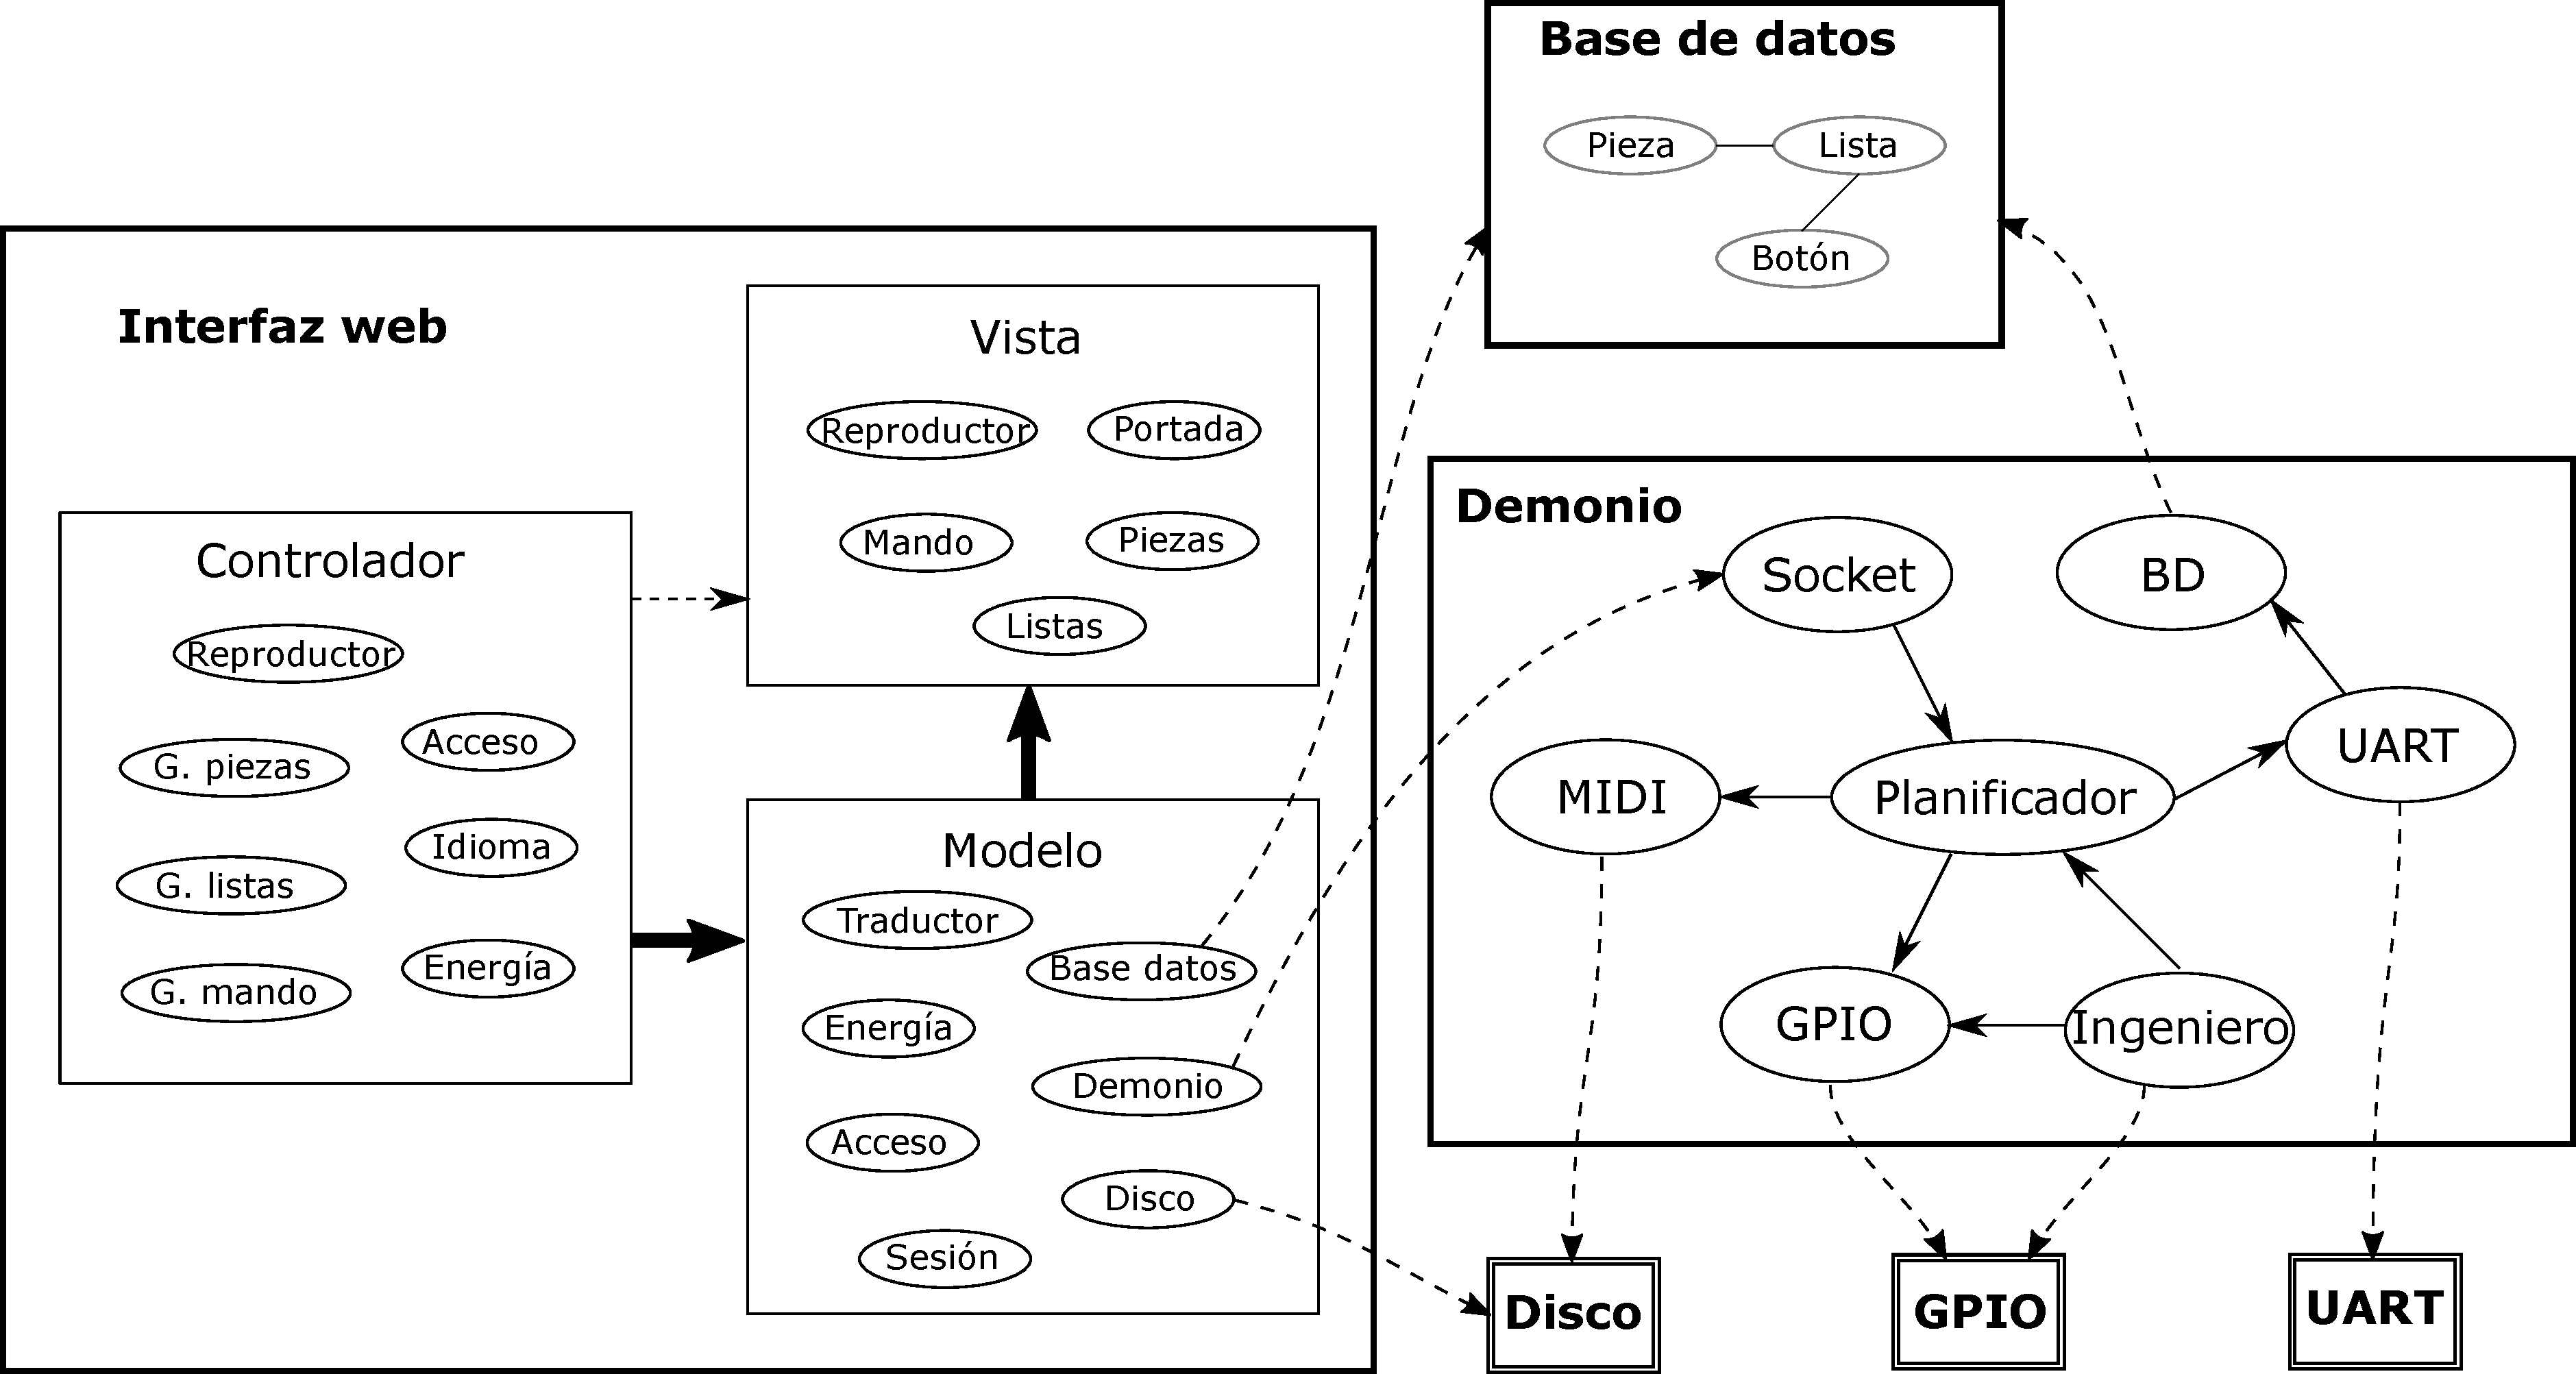
\includegraphics[width=0.75\textwidth]{images/sistema} 
		\captionof{figure}{Resumen del diseño del sistema.}
	\end{center}
	
	Al término de la fase de implementación hemos obtenido todo el sistema \textit{software} en distintos módulos y aplicaciones, que darán a la PCB todo el soporte especificado en los requisitos. La siguiente gráfica muestra la relación entre los 10 lenguajes utilizados:
	
	\begin{center}
		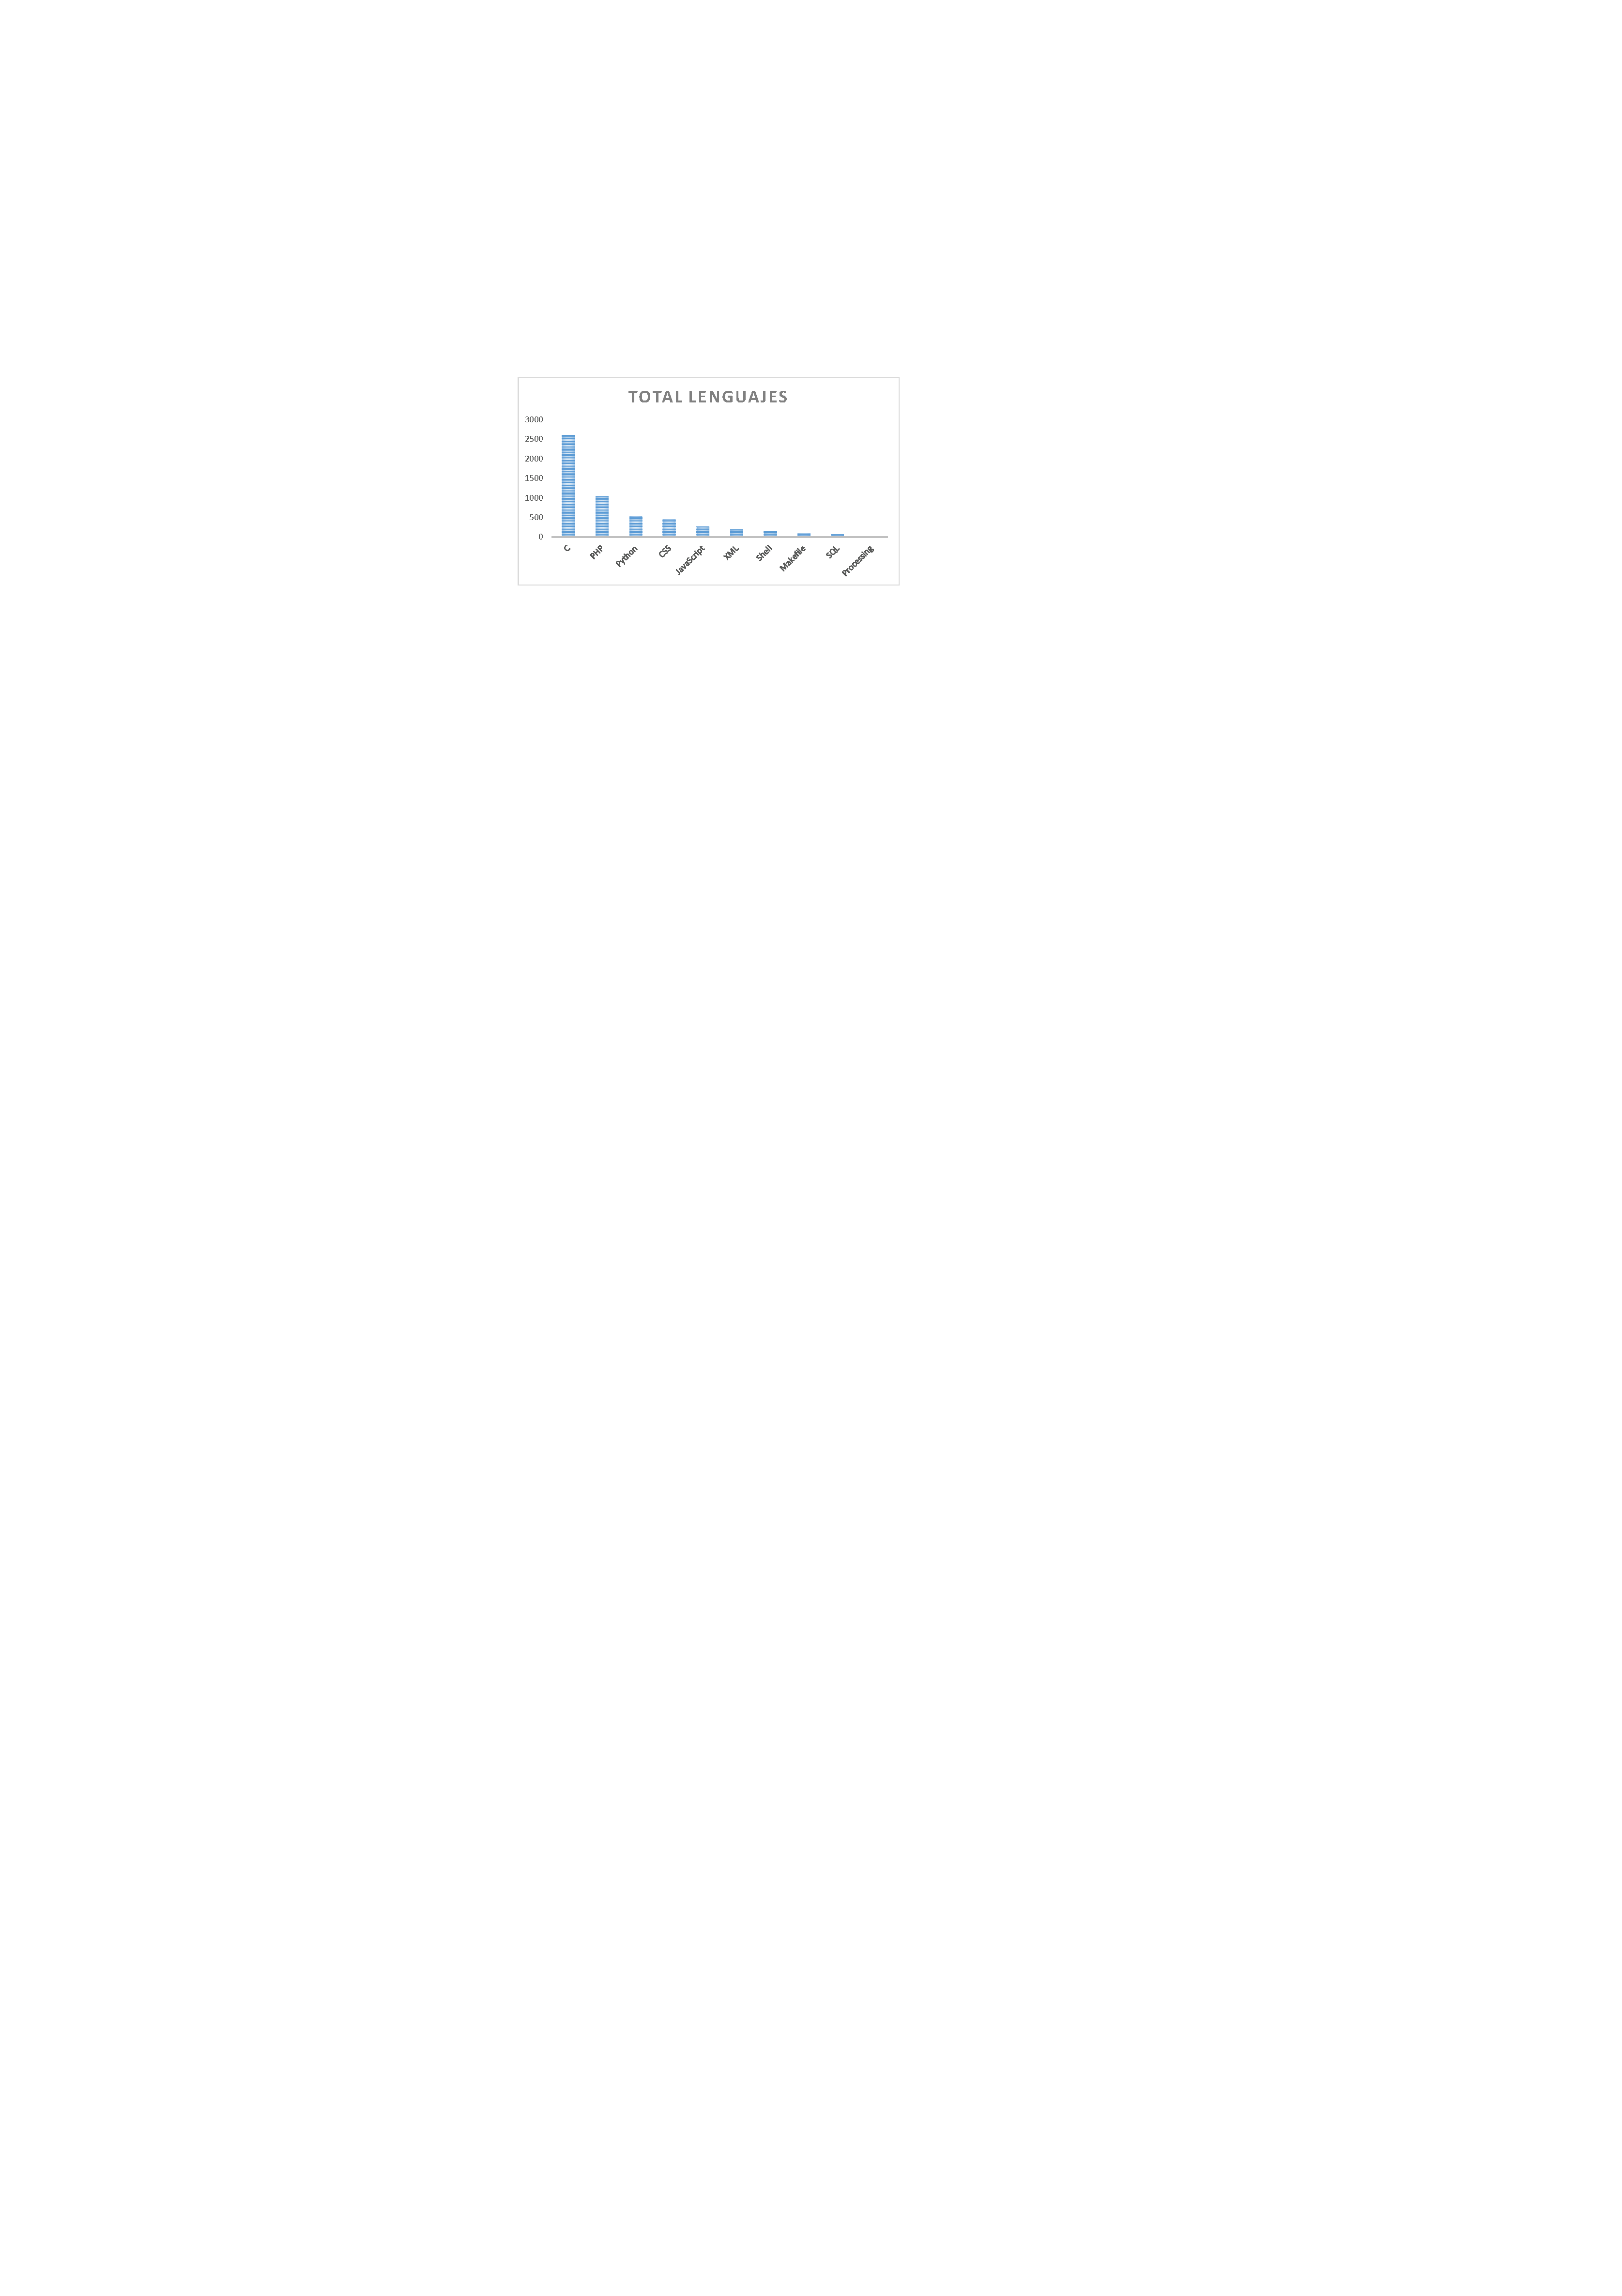
\includegraphics[width=0.75\textwidth]{images/lineas_lenguajes} 
		\captionof{figure}{Distribución del código fuente por lenguaje.}
	\end{center}
	
	% Capítulo 5 ---------------------------------------------------------------
	
	\section{Validación y verificación}
	
	Como fase final de cualquier proyecto, una vez terminada la implementación, es el momento de ejecutar las pruebas de validación sobre el sistema desarrollado.
	
	\subsection{Servicio de reproducción}
	
	El servicio de reproducción es el \textbf{demonio} desarrollado para reproducir las partituras y despachar peticiones del \textit{socket} y del mando (a través del UART). Ya que funcionará en segundo plano será muy importante que la implementación controle adecuadamente todos los errores posibles para evitar cierres inesperados.
	
	Algunos de los problemas más comunes son los \textbf{errores de memoria}, sobre todo en un lenguaje que no la gestiona automáticamente. Para validar la gestión de memoria, hemos utilizado la herramienta \textbf{Valgrind}, que nos muestra todos los posibles errores relativos a memoria.
	
	\subsubsection*{Entrada de archivos MIDI}
	
	El principal requisito del analizador de MIDI es que debe aceptar cualquier fichero de formato válido, no solo aquellos adaptados a nuestro proyecto. Hemos analizado hasta \textbf{46 archivos} MIDI de diferentes orígenes.
	
	De acuerdo a lo especificado, el \textit{software} analiza correctamente archivos MIDI con varias \textbf{pistas simultáneas}, y de cualquier \textbf{división de tiempo}, descartando los \textbf{eventos específicos} del sistema.
	
	Hemos medido 5 veces el tiempo de análisis de \textbf{10 partituras}, con el siguiente resultado:
	
	\begin{center}
		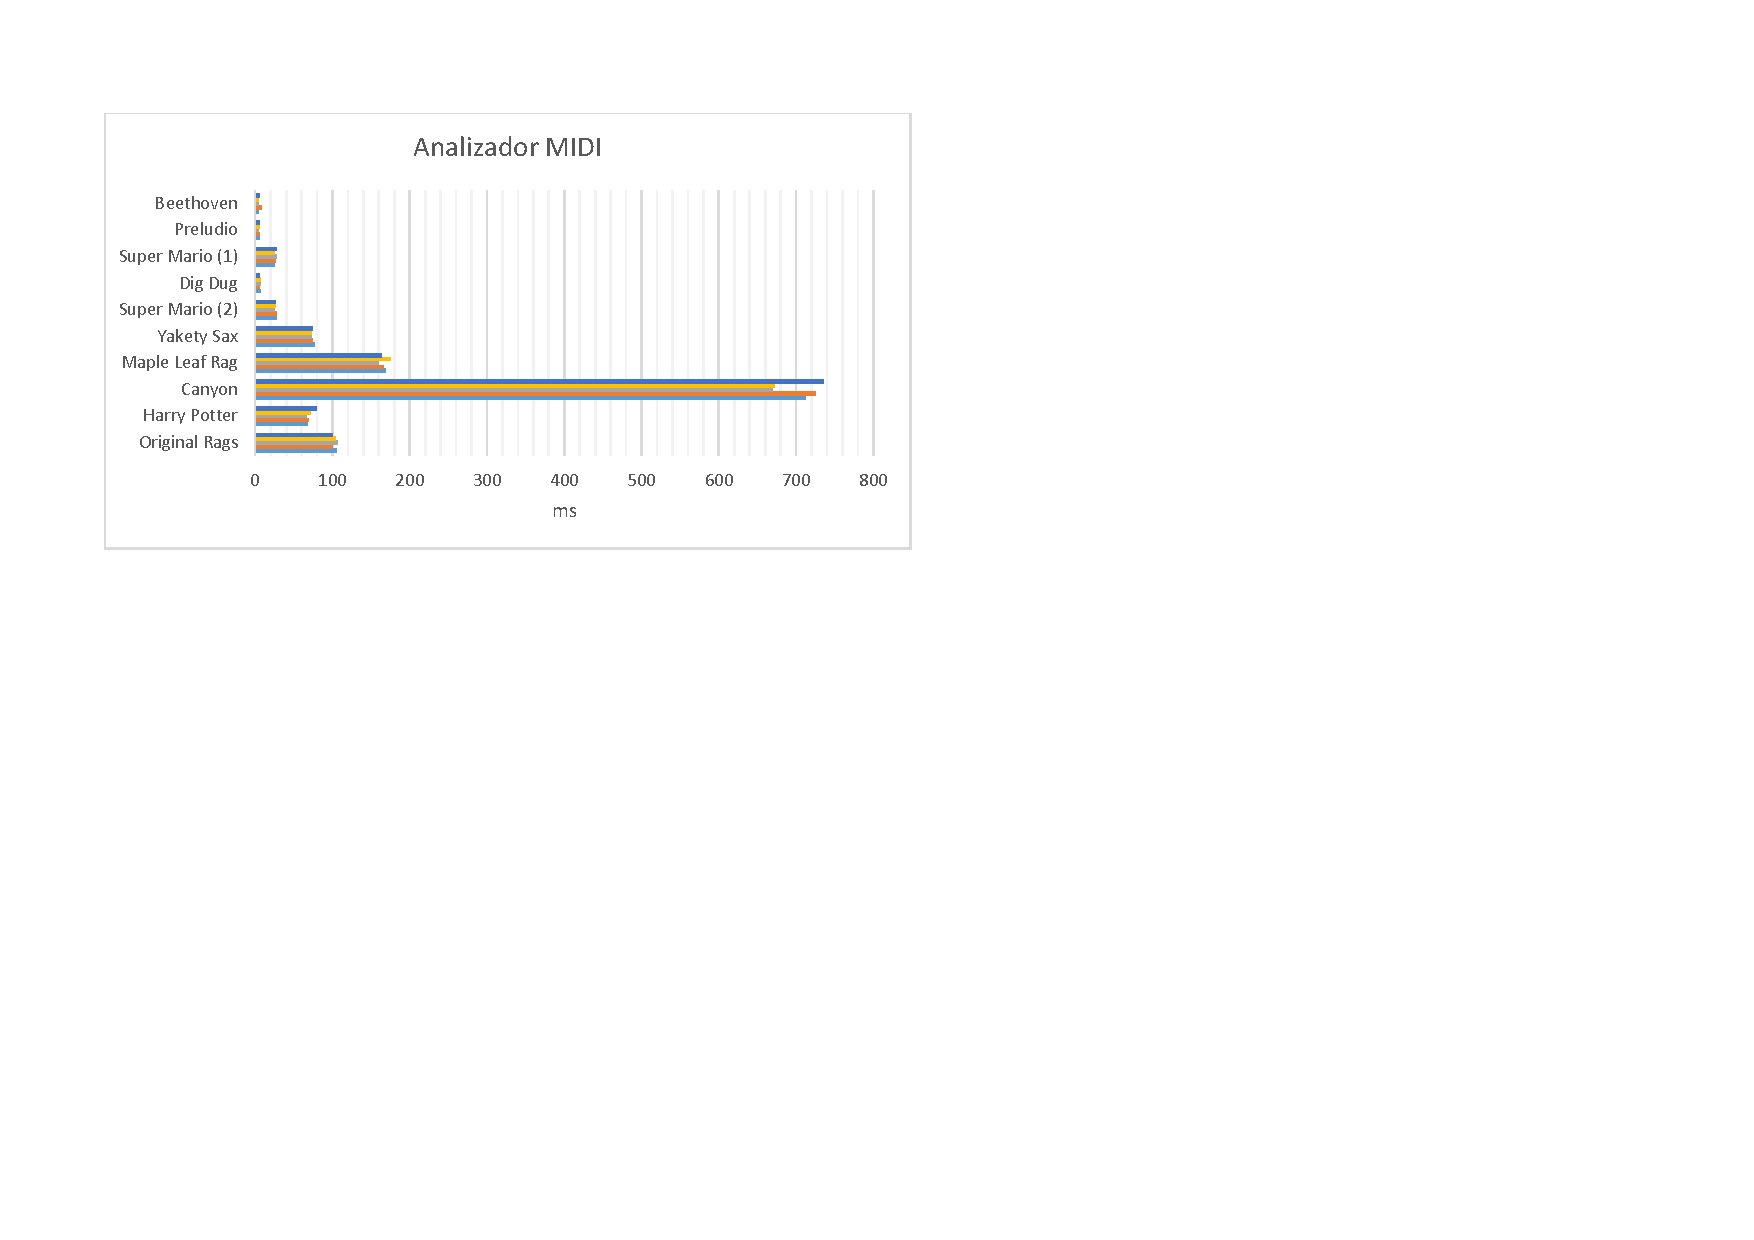
\includegraphics[width=0.75\textwidth]{images/lat_midi} 
		\captionof{figure}{Tiempo de ejecución del analizador MIDI.}
	\end{center}
	
	\subsubsection*{Planificador y control}
	
	El planificador debe ser capaz de atender ágilmente cualquier archivo MIDI con varias pistas. Para probarlo, utilizamos el \textbf{simulador} de reproducción, construido para este propósito. Esta aplicación fue muy útil para pulir cualquier detalle de programación, y probó que el \textbf{diseño} del algoritmo de planificación es correcto desde el primer momento.
	
	El concepto de la \textbf{interfaz de salida} también fue comprobado, a pesar de que la verificación de la implementación requiere la PCB, de la que dispondremos más adelante.
	
	Para analizar el rendimiento del planificador, medimos el \textbf{tiempo de cada iteración} del bucle principal. Para obtener los datos más adecuados al funcionamiento real, utilizaremos dos partituras específicas: la \textit{Oda a la Alegría} de Beethoven y el \textit{Preludio nº 4} de Bach:
	
	\begin{center}
		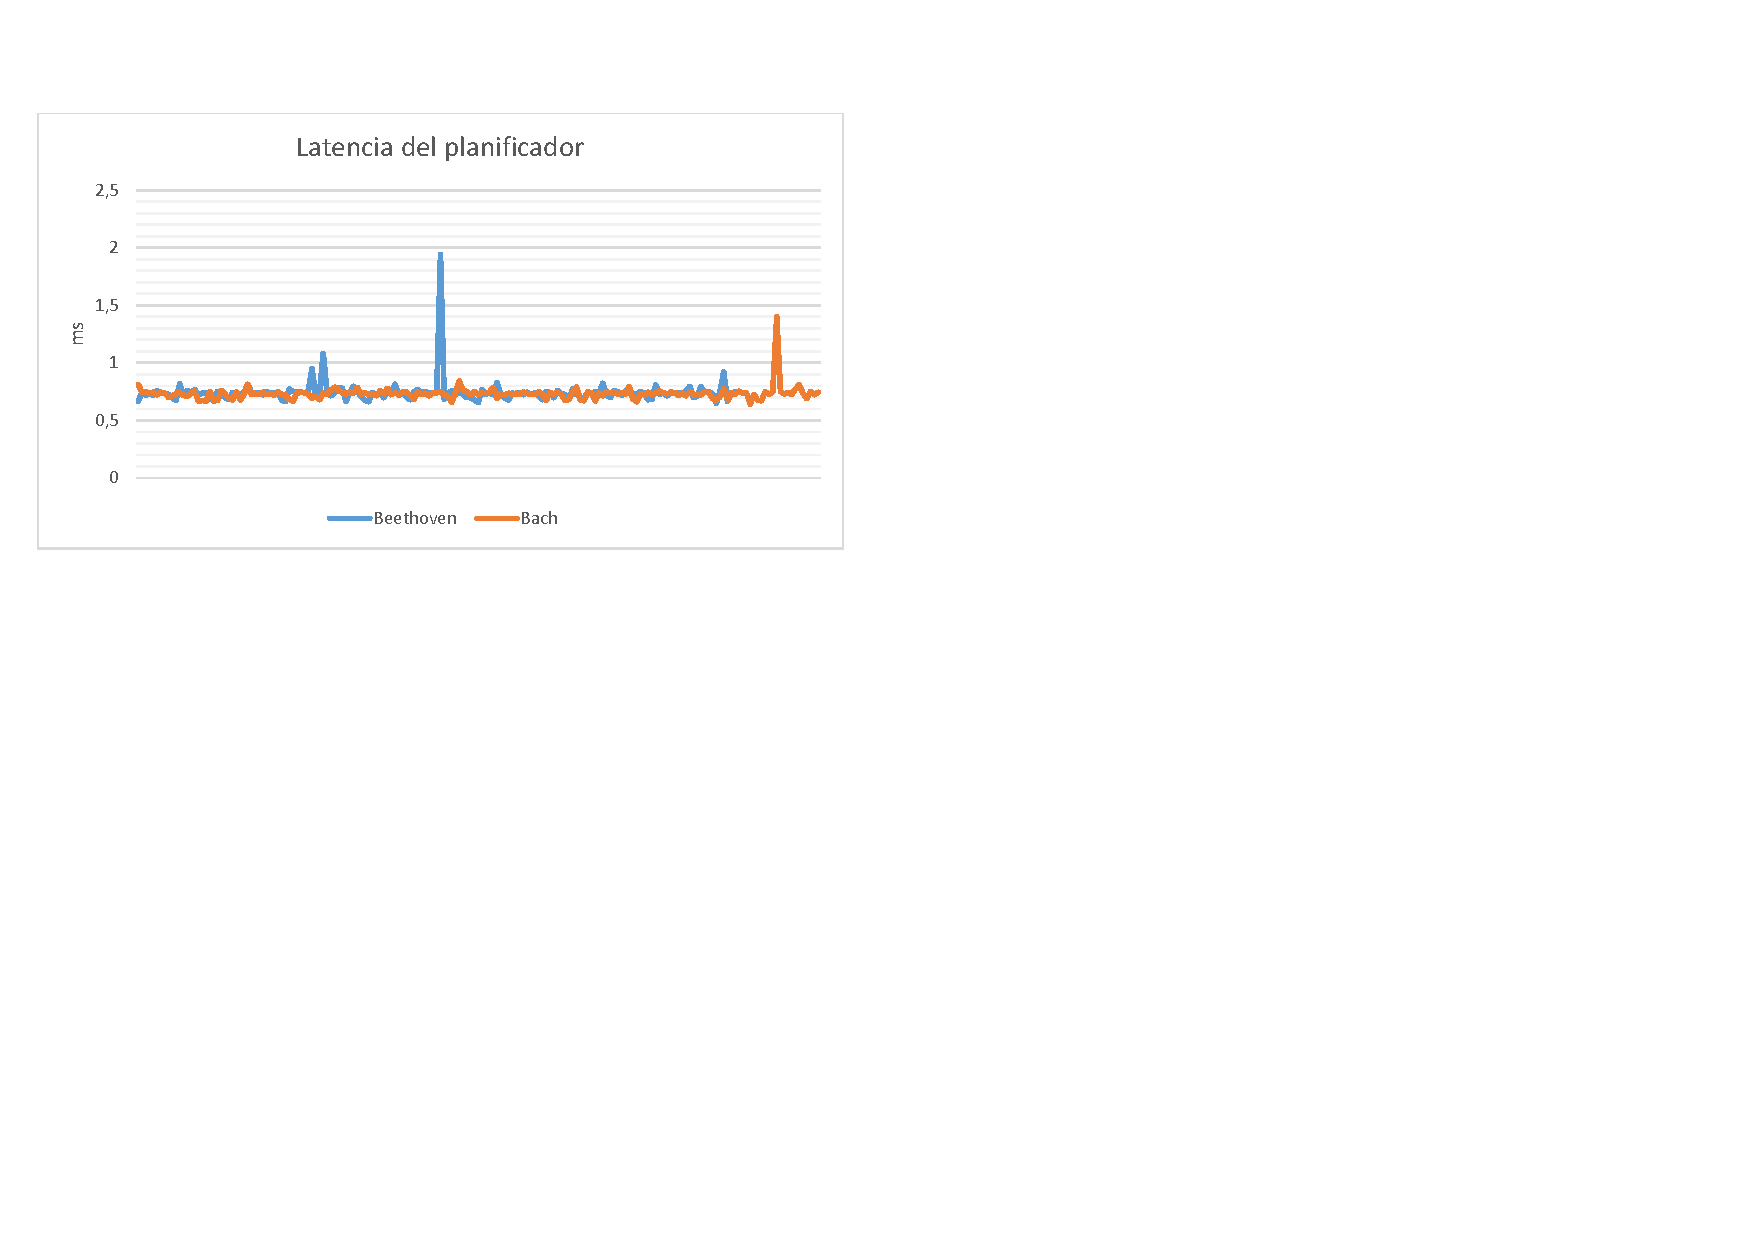
\includegraphics[width=0.75\textwidth]{images/lat_sched} 
		\captionof{figure}{Tiempo de ejecución del planificador.}
	\end{center}
	
	Los datos indican que el \textbf{ciclo medio} tarda $738 \; \mu s$. llegando hasta 1,94 \textit{ms}, un lapso imperceptible por el usuario.
	
	Es ahora el momento de medir el tiempo que tarda el programa en enviar los datos a la PCB a través del GPIO. En este caso, vamos a contrastar los datos del prototipo en Python y la implementación final en C:
	
	\begin{center}
		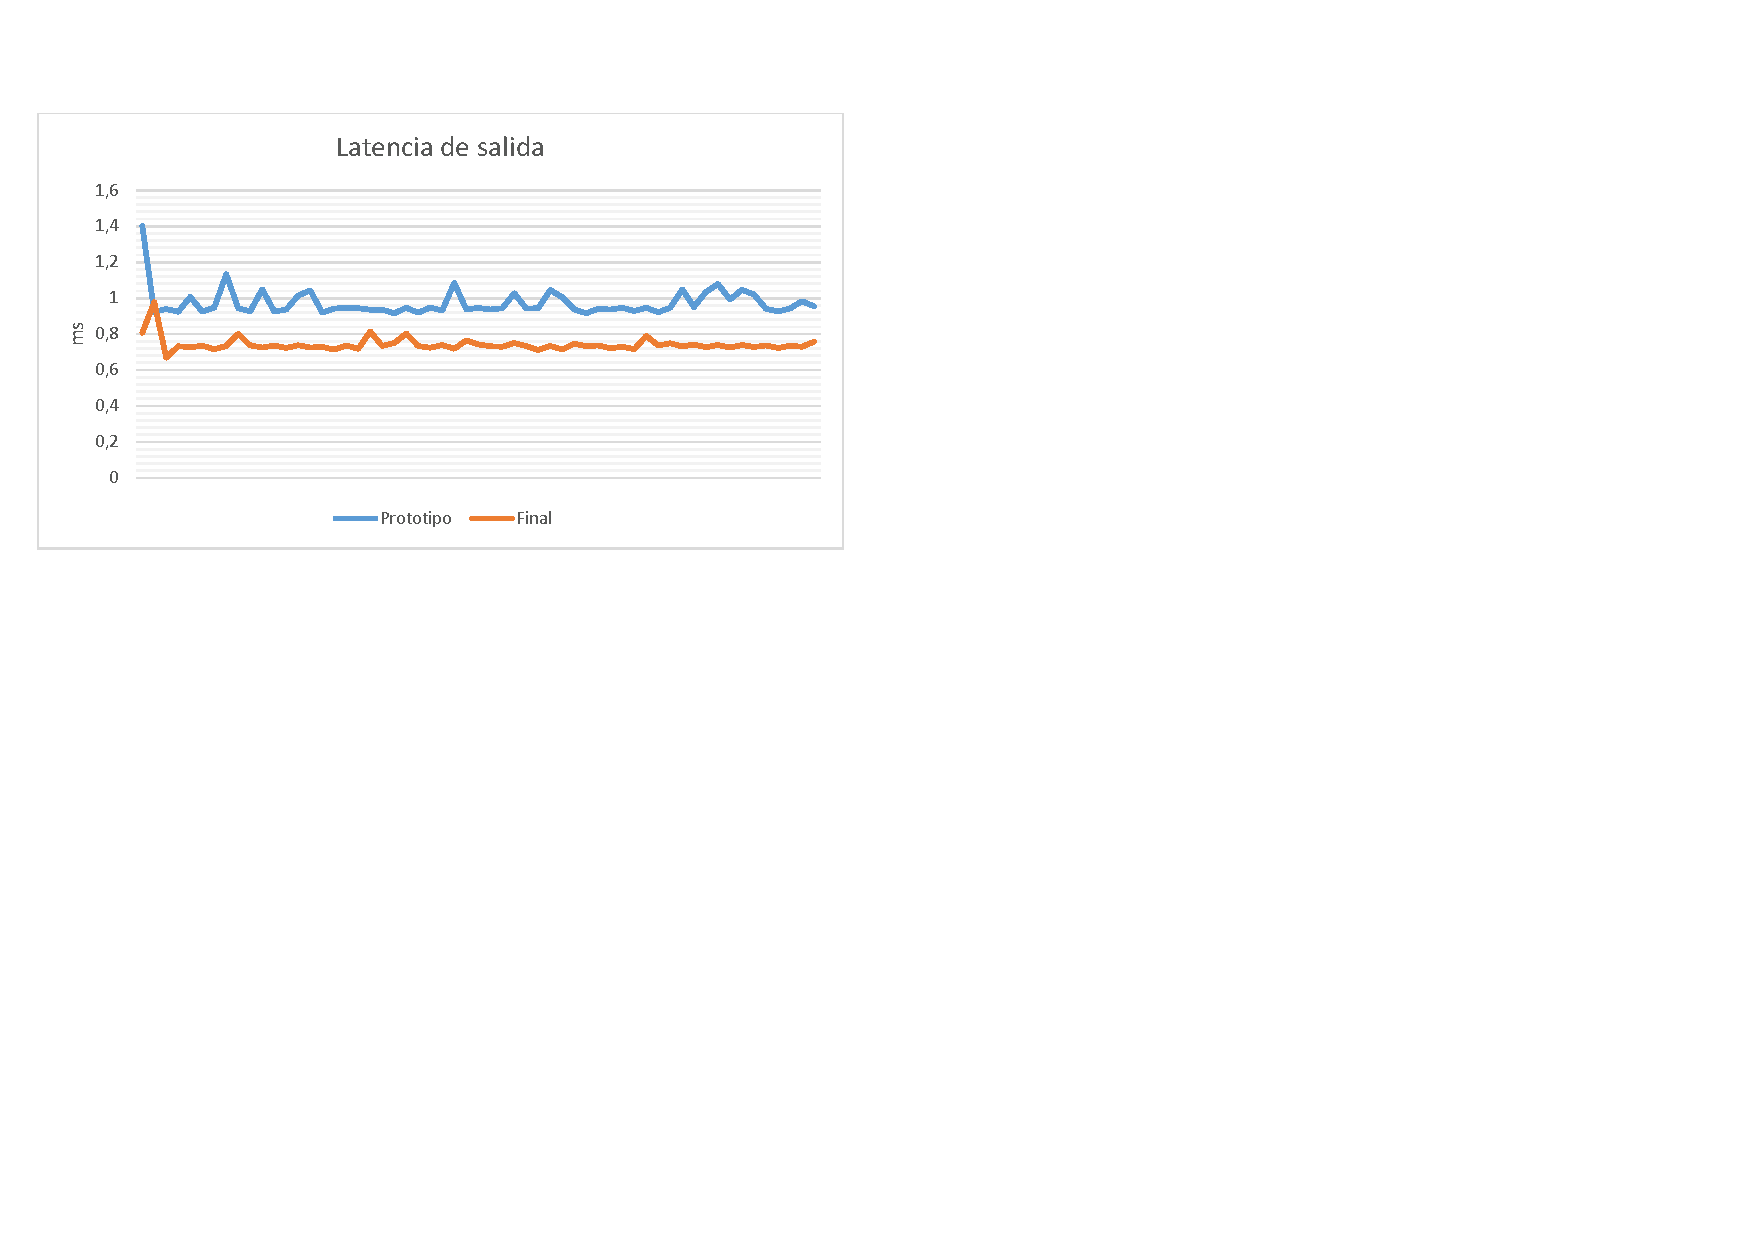
\includegraphics[width=0.75\textwidth]{images/lat_gpio} 
		\captionof{figure}{Tiempo de ejecución de la salida a GPIO.}
	\end{center}
	
	Por otro lado, la aplicación del \textbf{terminal} nos sirvió para dos cosas:
	
	\begin{enumerate}
		\item Verificar el \textbf{protocolo} de comunicación.
		\item Validar la gestión \textbf{concurrente} entre la hebra de reproducción y la del \textit{socket}.
	\end{enumerate}
	
	En base a las pruebas realizadas, el funcionamiento coincide con lo esperado, y controla adecuadamente los problemas en la entrada, tales como argumentos incorrectos o demasiado largos.
	
	\subsubsection*{Mando y metrónomo}
	
	La validación de esta parte del sistema requería disponer de la PCB, pero tenía una complejidad considerable y era necesario realizar incluso prototipos de \textit{software} para el UART.
	
	La solución a este problema fue utilizar un \textbf{\textit{Arduino}} para simular el mando a distancia, y un LED para comprobar el funcionamiento del metrónomo.
	
	Programamos una \textbf{batería de pruebas} para que Arduino suplantara al mando generando distintas cadenas aleatorias, variando los siguientes parámetros:
	
	\clearpage
	
	\begin{multicols}{2}
		\begin{enumerate}[nosep,itemsep=1em]
			\item Número de serie del mando.
			\item Botones pulsados.
			\item Señal de batería baja.
			\item Longitud de la cadena (generar errores).
		\end{enumerate}
		\columnbreak
		\begin{center}
			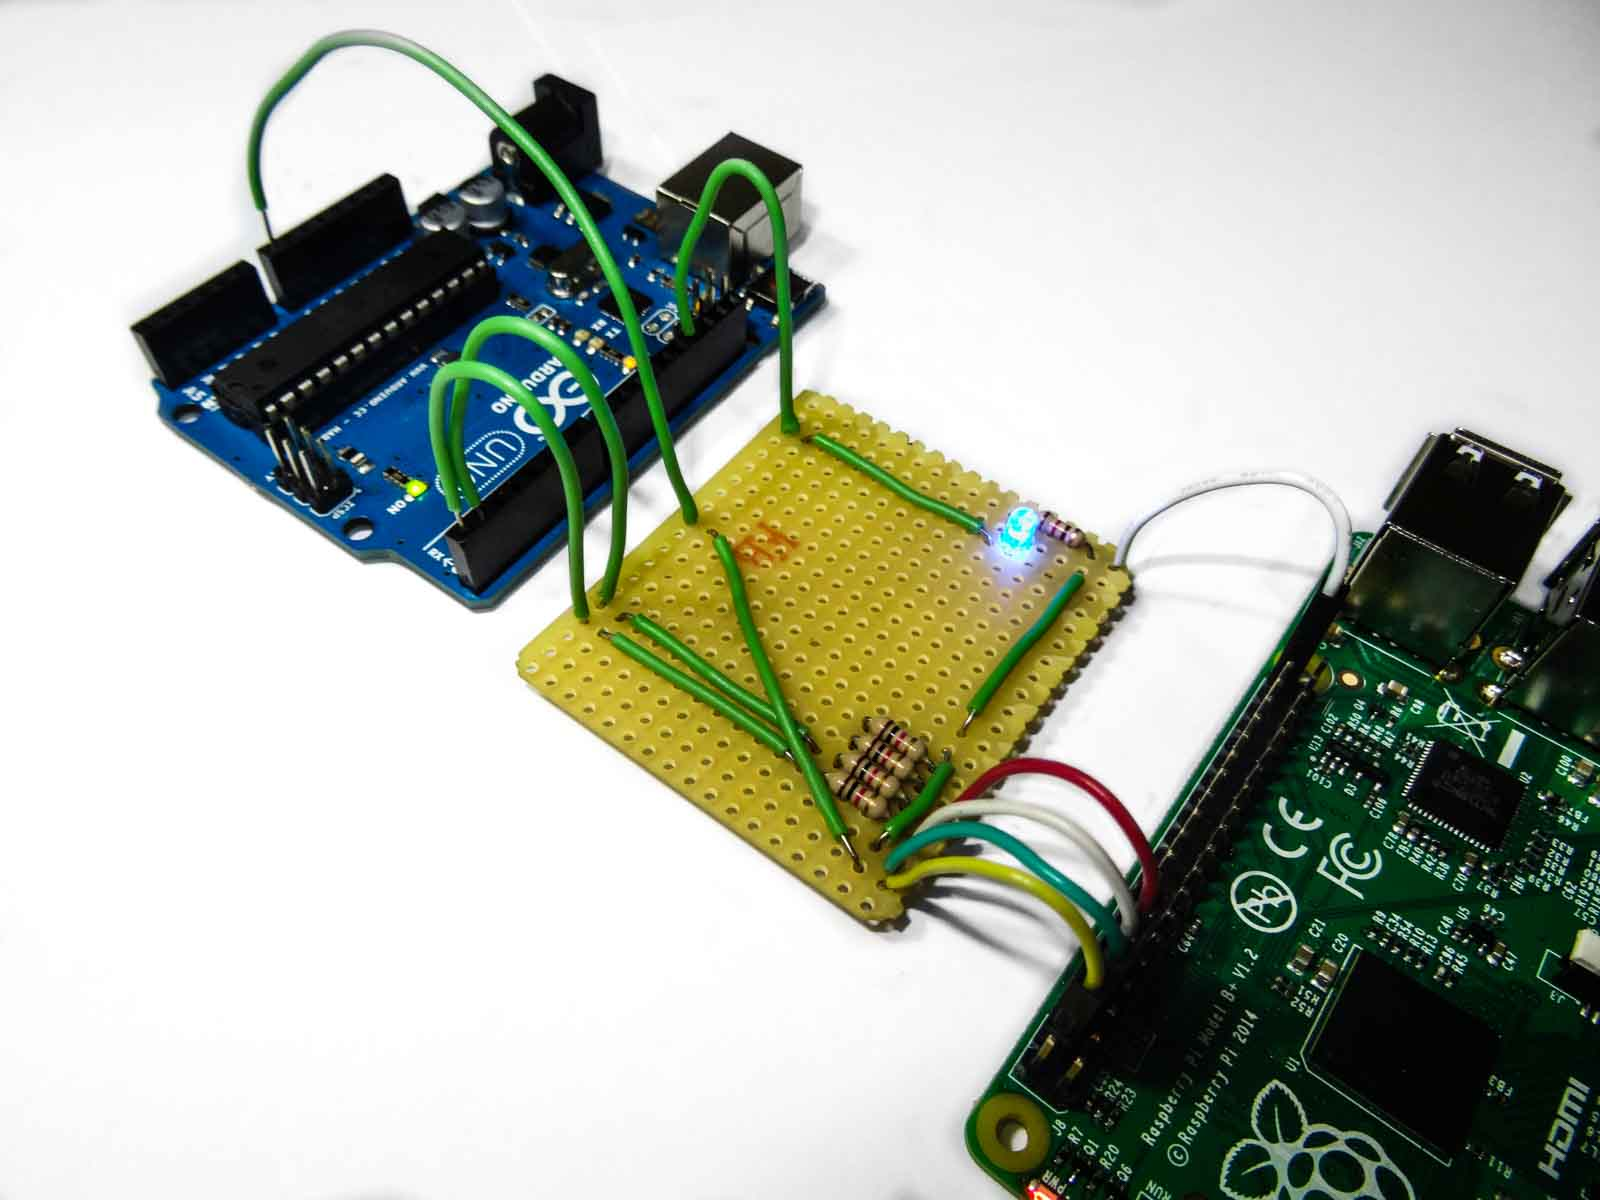
\includegraphics[width=0.45\textwidth]{images/proto_uart} 
			\captionof{figure}{Simulación del UART.}
		\end{center}
	\end{multicols}

	\subsection{Interfaz web}
	
	Ya que ésta es una aplicación de usuario, desplegaremos las pruebas típicas de entradas de datos en formularios. Una regla importante de la \textbf{programación defensiva} es no permitir al usuario utilizar incorrectamente el sistema.
	
	Además, podremos conectarnos desde \textbf{varios clientes} para comprobar que el sistema responde correctamente ante \textbf{peticiones simultáneas}.
	
	\subsubsection*{Vista y controlador}
	
	La implementación de las interfaces de entrada y salida sigue este principio:
	
	\begin{itemize}
		\item Si un error proviene del \textbf{usuario}, se comporta asertivamente (muestra un error).
		\item Si procede de un \textbf{error interno}, actúa pasivamente o muestra un error genérico.
	\end{itemize}
	
	\subsubsection*{Formularios}
	
	Los formularios tienen una \textbf{doble capa} de seguridad:
	 
	\begin{enumerate}
		\item La \textbf{vista} en HTML configura los campos para alertar al usuario si deja alguno en blanco o se excede del límite. El formulario \textbf{no se acepta} hasta que todas las entradas cumplan las condiciones.
	 	
	 	\item El \textbf{controlador} vuelve a comprobar las longitudes de cadena, filtra los mensajes para evitar \textbf{inyección de código}, y muestra un error si algún dato no está conforme.
	\end{enumerate}
	
	\clearpage
	\subsection{Prueba sobre la PCB}
	
	En último lugar, volvemos a reunirnos con Mikel Aguayo para validar nuestros \textbf{proyectos en conjunto}, tal como teníamos previsto. Actualmente solo disponemos de un \textbf{prototipo} del circuito impreso diseñado, más que suficiente para comprobar que el sistema funciona y se comporta como esperábamos.
	
	\subsubsection*{Entrada de datos}
	
	Sobre la placa hemos probado dos \textbf{versiones} del \textit{software}:
	
	\begin{enumerate}
		\item \textbf{Prototipo} en Python con una combinación fija de notas, como prueba de concepto.
		\item Implementación \textbf{final} del módulo \textit{software} de salida por GPIO.
	\end{enumerate}
	
	\begin{multicols}{2}
		En el prototipo establecimos un \textbf{ancho de pulso} muy grande, para descartarlo de antemano de cualquier otro problema que pudiera surgir. 
		
		La primera \textbf{prueba de concepto} fue satisfactoria, aunque producía errores en la salida, debido a desfases producidos por el intérprete Python.
		
		Utilizamos un \textbf{osciloscopio} para realizar medidas sobre las señales que el \textit{software} envía a la PCB.
		\columnbreak
		\begin{center}
			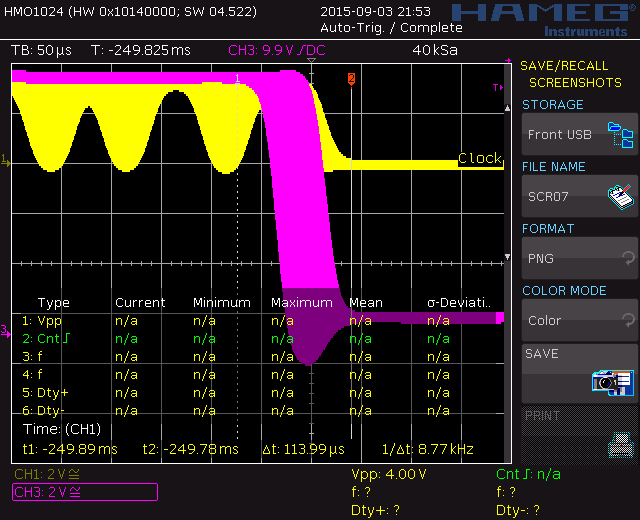
\includegraphics[width=0.45\textwidth]{images/osc_pulso} 
			\captionof{figure}{Ancho de pulso.}
		\end{center}
		
	\end{multicols}
	
	\subsubsection*{Modo Ingeniería}
	
	Éste es el nombre que hemos acuñado para el \textbf{control reducido}, que facilita un menú con cuatro funciones:
	
	\begin{multicols}{2}
		\begin{enumerate}[nosep,itemsep=1em]
			\item Ver el estado del \textbf{reproductor}.
			\item Controlar el \textbf{modo Ingeniería}.
			\item Activar el \textbf{metrónomo}.
			\item \textbf{Apagar} y reiniciar el sistema.
		\end{enumerate}
		\columnbreak
		\begin{center}
			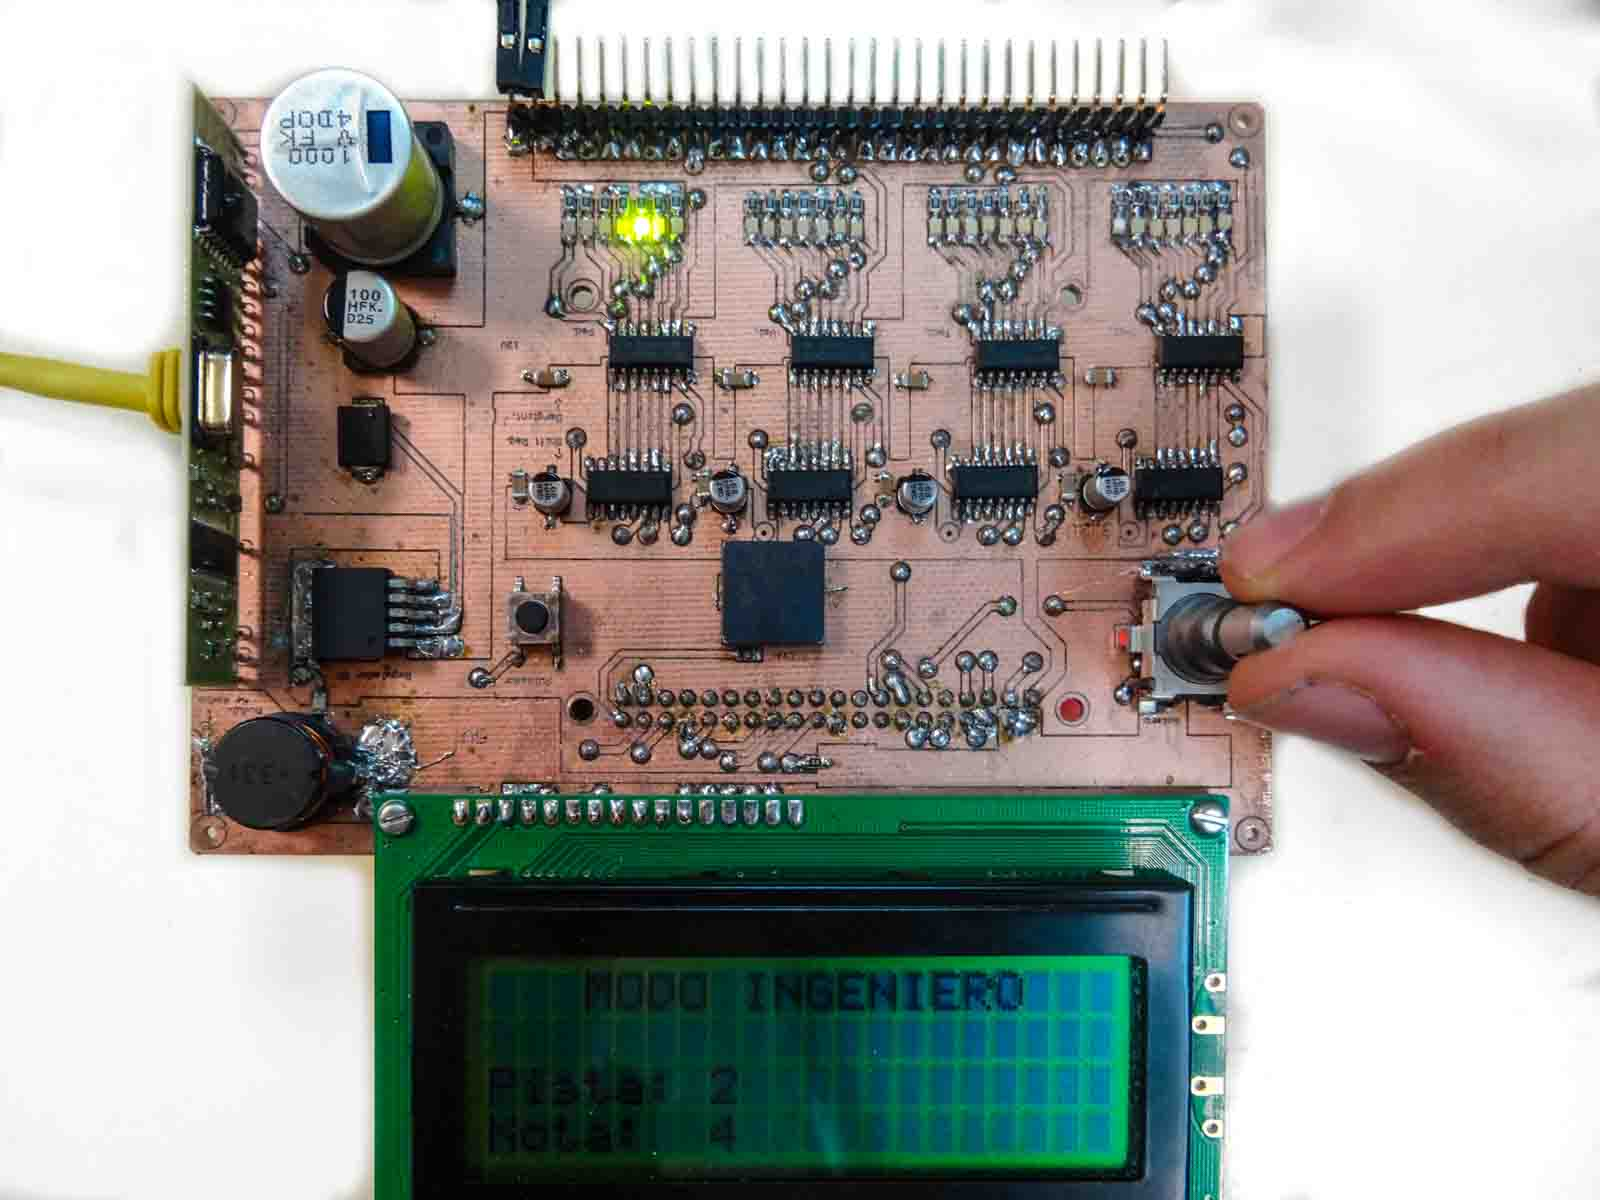
\includegraphics[width=0.45\textwidth]{images/pcb_ingeniero} 
			\captionof{figure}{PCB en modo Ingeniería.}
		\end{center}
		
	\end{multicols}
	
	% Capítulo 6 ---------------------------------------------------------------
		
	\section{Conclusión}
	
	Este proyecto ha supuesto, como era de esperar, el culmen de mi carrera universitaria, ya que ha abarcado \textbf{un poco de cada rama} de la informática. Esto me ha permitido repasar mis conocimientos, ampliarlos y desarrollar \textbf{nuevas capacidades}.
	
	Hemos conseguido, no solo diseñar el sistema, sino también llegar a hacer funcionar un \textbf{prototipo}, demostrando que el diseño es válido.
	
	No ha sido un trabajo sencillo, pero cada minuto que hemos dedicado ha merecido la pena, máxime al fusionar los dos proyectos hermanos y lograr dar vida al \textit{hardware} de la PCB. 
	
	Me siento honestamente satisfecho del trabajo realizado. Reitero mi agradecimiento a mi compañero Mikel, a mis tutores, y a todos los que nos han ayudado a llevar este proyecto adelante.
	
	\subsection{Vínculos}
	
	\begin{itemize}
		\item Repositorio en GitHub: \url{https://github.com/vikman90/organo}.
		\item Vídeo en YouTube: \url{https://www.youtube.com/watch?v=DHq1yLxVZu4}.
	\end{itemize}
\end{document}
